\documentclass[a4paper,11pt,twoside]{book} 
\usepackage{hyperref,fancyhdr,graphicx,amssymb,amsmath,times,makeidx,listings} 
\graphicspath{{img/}} 
\pagestyle{fancyplain} 
\lhead[\fancyplain{}{\textbf\thepage}]{\fancyplain{}{\rightmark}} 
\rhead[\fancyplain{}{\leftmark}]{\fancyplain{}{\textbf\thepage}} 
\cfoot{} 
\setlength{\textwidth}{5.875in} 
\setlength{\parindent}{0pc} 
\setlength{\hoffset}{-0.8cm} 
\setcounter{tocdepth}{1} 
\sloppy{} 
\title{\fbox{\parbox{\textwidth}{\begin{center}\vspace*{2cm}
\includegraphics[width=12cm]{logo3.jpg}\\\vspace*{1cm}{\Huge \textbf{The Handbook}\\{\small Version 1.5.8.1 (beta)}\\\vspace*{1cm}}\end{center}}}} 
\author{\Large \bf David Tschumperl\'e} 
\renewcommand\indexname{Index of commands} 
\makeindex 
\lstset{columns=fullflexible,basicstyle=\normalfont} 
\begin{document} 
\maketitle 
\tableofcontents 
\chapter*{Preamble} 
\section*{License} 
This document is distributed under the \textbf{GNU Free Documentation License}, version 1.3.\\ 
Read the full license terms at \texttt{http://www.gnu.org/licenses/fdl-1.3.txt}.\\~\\ 
An online version of this documentation is available at:\\\texttt{http://gmic.sourceforge.net/reference.shtml}. 
\section*{Motivations} 
G'MIC is an open and full-featured framework for image processing, providing several different user interfaces to 
convert/manipulate/filter/visualize generic image datasets, from 1d scalar signales to 3d+t sequences of multi-spectral volumetric images. 
Technically speaking, what it does is: 
\begin{itemize} 
\item Define a lightweight but powerful script language (the G'MIC language) dedicated to the design of image processing pipelines. 
\item Provide several user interfaces embedding the corresponding interpreter: 
\begin{itemize} 
\item A command-line executable 'gmic', to use the G'MIC framework from a shell. 
In this setting, G'MIC may be seen as a direct (and friendly) competitor of the ImageMagick or GraphicsMagick software suites. 
\item A plug-in 'gmic\_gimp', to bring G'MIC capabilities to the GIMP image retouching software. 
\item A web-service 'G'MIC Online', to allow users applying image processing algorithms directly in a web brower. 
\item A Qt-based interface 'ZArt', for real-time manipulation of webcam images. 
\item A C++ library 'libgmic', to be linked with third-party applications. 
\end{itemize} 
\end{itemize} 
G'MIC is focused on the design of possibly complex pipelines for converting, manipulating, filtering and visualizing generic 1d/2d/3d multi-spectral image datasets. This includes of course color images, but also more complex data as image sequences or 3d(+t) volumetric float-valued datasets.\\ 
 
G'MIC is an open framework: the default language can be extended with custom G'MIC-written commands, defining thus new available image filters or effects. By the way, G'MIC already contains a substantial set of pre-defined image processing algorithms and pipelines (more than 1000).\\ 
 
G'MIC has been designed with portability in mind and runs on different platforms (Windows, Unix, MacOSX). It is distributed under the CeCILL license (GPL-compatible). Since 2008, it is developed in the Image Team of the GREYC laboratory, in Caen/France, by permanent researchers working in the field of image processing on a daily basis. 
\section*{Version} 
 
 gmic: GREYC's Magic for Image Computing. 
 
        Version 1.5.8.1 (beta), Copyright (c) 2008-2013, David Tschumperl\'e 
        (http://gmic.sourceforge.net) 
\chapter{Usage} 
\small
\begin{lstlisting}
 gmic [command1 [arg1_1,arg1_2,..]] .. [commandN [argN_1,argN_2,..]] 
 
 'gmic' is an open-source interpreter of the G'MIC language, a script-based programming 
  language dedicated to design image processing pipelines. It can be used to convert, 
  manipulate, filter and visualize datasets made of one or several 1d/2d or 3d multi- 
  spectral images. 
 
 This documentation proposes a complete description of the G'MIC language basics and rules.
\end{lstlisting}
\normalsize
\section{Overall context}
\small
\begin{lstlisting}
  - At any time, G'MIC manages one list of numbered (and optionally named) pixel-based 
     images, entirely stored in computer memory. 
  - The first image of the list has indice '0' and is denoted by '[0]'. The second image of 
     the list is denoted by '[1]', the third by '[2]' and so on. 
  - Negative indices are treated in a cyclic way: '[-1]' refers to the last image of the 
     list, '[-2]' to the penultimate one, etc. Thus, if the list has 4 images, '[1]' and '[-3]' 
     both designate the second image of the list. 
  - A named image may be denoted by '[name]' if 'name' uses characters set [a-zA-Z0-9_] and 
     does not start with a number. Image names can be set or reassigned at any moment during 
     the processing pipeline (see commands '-name' and '-input'). 
  - G'MIC defines a set of various commands and substitution mechanisms to allow the design 
     of complex pipelines managing this list of images, in a very flexible way: 
     You can insert or remove images in the list, rearrange image indices, process images 
     (individually or as a group), merge image data together and output image files. 
  - Such a pipeline can be written itself as a custom G'MIC command storable in a custom 
     commands file, which can be re-used afterwards in another bigger pipeline if necessary.
\end{lstlisting}
\normalsize
\section{Image definition and terminology}
\small
\begin{lstlisting}
  - In G'MIC, an image is modeled as a 1d, 2d, 3d or 4d array of scalar values, uniformly 
     discretized on a rectangular/parallelepipedic domain. 
  - The four dimensions of these arrays are respectively denoted by: 
    . 'width', the number of image columns (size along the 'x'-axis). 
    . 'height', the number of image rows (size along the 'y'-axis). 
    . 'depth', the number of image slices (size along the 'z'-axis). 
        The depth is equal to 1 for usual 2d color or grayscale images. 
    . 'spectrum', the number of image channels (size along the 'c'-axis). 
        The spectrum is respectively equal to 3 and 4 for usual RGB and RGBA color images. 
  - There are no size limitations on each image dimensions. Particularly, the number of image 
     slices or channels can be of arbitrary size within the limits of available memory. 
  - The width, height and depth of an image are considered as 'spatial' dimensions, while the 
     spectrum has a 'multi-spectral' meaning. Thus, a 4d image in G'MIC should be most often 
     regarded as a 3d dataset of multi-spectral voxels. Most of the G'MIC commands will stick 
     with this idea (e.g. command '-blur' will blur images only along the 'xyz' axes). 
  - All pixel values of all images of the list have the same datatype. It can be one among: 
    . 'bool': Stands for 'boolean'. Value range is { 0=false | 1=true }. 
    . 'uchar': Stands for 'unsigned char'. Value range is [0,255] (8bits). 
        This type of pixel coding is commonly used to store 8bits/channels RGB[A] images. 
    . 'char': Value range is [-128,127] (8bits). 
    . 'ushort': Stands for 'unsigned short'. Value range is [0,65535] (16bits). 
        This type of pixel coding is commonly used to store 16bits/channels RGB[A] images. 
    . 'short': Value range is [-32768,32767] (16bits). 
    . 'uint': Stands for 'unsigned int'. Value range is [0,2^32-1] (32bits). 
    . 'int': Value range is [-2^31,2^31-1] (32 bits). 
    . 'float': Value range is [-3.4E38,+3.4E38] (32bits). 
        This type of coding is able to store pixels as 32 bits float-valued numbers. This is 
        the default datatype used by G'MIC image processing operations. 
    . 'double': Value range is [-1.7E308,1.7E308] (64bits). 
        This type of coding is able to store pixels as 64 bits float-valued numbers. 
  - Considering pixel datatypes different than 'float' is generally useless, except to force 
     the input/output of image data to a prescribed binary format. Hence, most G'MIC image 
     image processing commands are available only for the default 'float' pixel datatype 
     (see command '-type' if you need to switch to another pixel datatype).
\end{lstlisting}
\normalsize
\section{Items of a processing pipeline}
\small
\begin{lstlisting}
  - In G'MIC, an image processing pipeline is described as a sequence of items separated by 
     the space character ' '. Such items are interpreted and executed from the left to the 
     right. For instance, the expression: 
       'input.jpg -blur 3,0 -sharpen 10 -resize 200%,200% -output output.jpg' 
     defines a valid pipeline composed of nine G'MIC items. 
  - A G'MIC item is a string which represents either a command, a set of command arguments, 
     a filename, or a special input string. 
  - Escape characters '\' and double quotes '"' can be used (as usual) to define items 
     containing spaces, or any other character sequences. For instance, the strings 
     'single\ item' and '"single item"' define the same string item, with a space in it.
\end{lstlisting}
\normalsize
\section{Input data items}
\small
\begin{lstlisting}
  - If a specified G'MIC item appears to be an existing filename, the corresponding image 
     data are loaded and inserted at the end of the image list. 
  - Special filenames '-' and '-.ext' stand for the standard input/output streams, optionally 
     forced to be in a specific 'ext' file format (e.g. '-.jpg' or '-.png'). 
  - The following special input strings may be used as G'MIC items to create and insert new 
     images with prescribed values, at the end of the image list: 
    . '[selection]' or '[selection]xN': Insert 1 or N copies of selected existing images. 
       'selection' may contain one or several images (see next section for details). 
    . 'width[%],_height[%],_depth[%],_spectrum[%],_values': Insert a new image with 
       specified size and values (adding '%' to a dimension means 'percentage of the size 
       along the same axis, taken from the last image '[-1]''). Any specified dimension 
       can be also written as '[image]', and is then set to the size (along the same axis) 
       of the existing specified image [image]. 'values' can be either a sequence of numbers 
       separated by commas ',', or a mathematical expression, as e.g. in input item 
       '256,256,1,3,if(c==0,x,if(c==1,y,0))' which creates a 256x256 RGB color image with a 
       spatial shading on the red and green channels. 
    . '(v1,v2,..)': Insert a new image from specified prescribed values. 
       Value separator inside parentheses can be ',' (column separator.), ';' (row sep.), 
       '/' (slice sep.) or '^' (channel sep.). For instance, expression 
       '(1,2,3;4,5,6;7,8,9)' creates a 3x3 matrix (scalar image), with values from 1 to 9. 
    . '0': Insert a new 'empty' image, containing no pixel data. Empty images are used only 
       in rare occasions. 
  - Input item 'name=value' declares a new local or global variable 'name', or assign a new 
     value to an existing variable. Variable names use characters set [a-zA-Z0-9_] and cannot 
     start with a number. A variable definition is always local to the current command except 
     when it starts by the underscore character '_'. In that case, it becomes also accessible 
     by any command invoked outside the current command scope.
\end{lstlisting}
\normalsize
\section{Command items and selections}
\small
\begin{lstlisting}
  - A G'MIC item starting by '-' designates a command, most of the time. Generally, commands 
     perform image processing operations on one or several available images of the list. 
  - Common commands have two equivalent names (regular and short). For instance, command 
     names '-resize' and '-r' refer to the same image resizing action. 
  - A G'MIC command may have mandatory or optional arguments. Command arguments must be 
     specified in the next item on the command line. Commas ',' are used to separate multiple 
     arguments, if any required. 
  - The execution of a G'MIC command may be restricted only to a subset of the image list, by 
     appending '[subset]' to the command name. Examples of valid syntaxes for 'subset' are: 
    . '-com[0,1,3]': Apply command only on images [0],[1] and [3]. 
    . '-com[3-5]': Apply command only on images [3] to [5] (i.e, [3],[4] and [5]). 
    . '-com[50%-100%]': Apply command only on the second half of the image list. 
    . '-com[0,-4--1]': Apply command only on the first and the four latest images. 
    . '-com[0-9:3]': Apply command only on images [0] to [9], with a step of 3 
                      (i.e. on images [0], [3], [6] and [9]). 
    . '-com[0--1:2]': Apply command only on images of the list with even indices. 
    . '-com[0,2-4,50%--1]': Apply command on images [0],[2],[3],[4] and on the second half 
                             of the image list. 
    . '-com[^0,1]': Apply command on all images except the first two. 
    . '-com[name1,name2]': Apply command on named images 'name1' and 'name2'. 
  - Indices in selections are always sorted in increasing order, and duplicate indices are 
     discarded. For instance, selections '[3-1,1-3]' and '[1,1,1,3,2]' are both equivalent to 
     '[1-3]'. If you want to repeat a single command multiple times on an image, use a 
     '-repeat..-done' loop. Inverting the order of images in a selection can be achieved by 
     inverting first the order of the images in the list, with command '-reverse[selection]'. 
  - G'MIC commands invoked without '[subset]' are applied on all images of the list. 
  - A G'MIC command starting with '--' instead of '-' does not act 'in-place' but inserts its 
     result as one or several new images at the end of the image list. 
  - There are two different types of commands that can be run by the G'MIC interpreter: 
    . Native commands, are hard-coded functionalities in the interpreter core. 
       They are thus compiled as machine code and run quickly, most of the time. 
       Omitting an argument when invoking a native command is not permitted, except if all 
       following arguments are also omitted. For instance, call to '-plasma 10,,5' is invalid 
       but '-plasma 10' is correct. 
    . Custom commands, are defined as G'MIC pipelines of native or custom commands. 
       They are interpreted by the G'MIC interpreter, and run slower than native commands. 
       But omitting arguments when invoking a custom command is permitted. For instance, 
       expressions '-flower ,,,100,,2' or '-flower ,' are correct. 
  - A user may easily add its own custom commands to the G'MIC interpreter (see section 
     'Adding custom commands'). Native commands cannot be added unless you modify the G'MIC 
     interpreter source code.
\end{lstlisting}
\normalsize
\section{Inputs / outputs properties}
\small
\begin{lstlisting}
  - G'MIC is able to read/write most of the classical image file formats, including: 
    . 2d grayscale/color files: .png, .jpeg, .gif, .pnm, .tif, .bmp, .. 
    . 3d volumetric files: .dcm, .hdr, .nii, .pan, .inr, .pnk, .. 
    . Image sequences: .mpeg, .avi, .mov, .ogg, .flv, .. 
    . Generic ascii or binary data files: .cimg, .cimgz, .dlm, .asc, .pfm, .raw, .txt, .h. 
    . 3d object files: .off. 
  - When dealing with color images, G'MIC generally reads, writes and displays data using the 
     usual RGB color space. 
  - G'MIC is able to manage 3d objects that may be read from files or generated by G'MIC 
     commands. They are stored as one-column scalar images containing the object data, in the 
     following order: { magic_number; sizes; vertices; primitives; colors; opacities }. 
     These 3d representations can be processed as regular float-valued images. 
     (see command '-split3d' for accessing each of these 3d object data separately). 
  - Be aware that usual file formats may be sometimes not adapted to store all the available 
     image data, since G'MIC uses float-valued coding of image pixels. For instance, saving 
     an image that was initially loaded as a 16bits/channel image, as a .jpg file will result 
     in loss of information. Use the .cimg file extension (or .cimgz, its compressed 
     version) to ensure that all data precision will be preserved when saving images. 
  - File options can/must be set for these specific file formats: 
    . Video files: Only sub-frames of an image sequence may be loaded, using the input 
       expression 'filename.ext,[first_frame[%][,last_frame[%][,step]]]'. 
       Output framerate and bitrate (in Kb/s) can be also set by using the output expression 
       'file.mpg,_fps,_bitrate'. 
    . .cimg files : Only crops and sub-images of .cimg files can be loaded, using the input 
      expressions 'filename.cimg,N0,N1', 'filename.cimg,N0,N1,x0,x1', 
      'filename.cimg,N0,N1,x0,y0,x1,y1', 'filename.cimg,N0,N1,x0,y0,z0,x1,y1,z1', 
      'filename.cimg,N0,N1,x0,y0,z0,c0,x1,y1,z1,c1'. 
      Specifying '-1' for one coordinates stands for the maximum possible value. 
    . .raw binary files: Image dimensions and input pixel type may be specified when loading 
       .raw files with input expresssion 'filename.raw[,type][,width][,height[,depth[,dim]]]]'. 
       If no dimensions are specified, the resulting image is a one-column vector with 
       maximum possible height. Pixel type can also be specified with the output 
       expression 'file.raw[,type]'. 
       'type' can be { bool | uchar | char | ushort | short | uint | int | float | double }. 
    . .yuv files: Image dimensions must be specified, and only sub-frames of an image 
       sequence may be loaded, using the input expression 
      'filename.yuv,width,height[,first_frame[,last_frame[,step]]]'. 
    . .tiff files: Only sub-images of multi-pages tiff files can be loaded, using the input 
       expression 'filename.tif,[first_frame,[last_frame,[step]]]'. 
    . .gif files: Animated gif files can be saved, using the input expression 
      'filename.gif,fps,nb_loops'. 
      Specify 'nb_loops=0' to get an infinite number of animation loops. 
    . .jpeg files: The output quality may be specified (in %), using the output expression 
       'filename.jpg,30' (here, to get a 30% quality output). 
    . .mnc files: The output header can set from another file, using the output expression 
       'filename.mnc,header_template.mnc'. 
    . Filenames with extension '.gmic' are assumed to be G'MIC custom commands files. Loading 
       such a file will add the commands it defines to the interpreter. 
    . Inserting 'ext:' on the beginning of a filename (e.g. 'jpg:filename') forces G'MIC to 
       read/write the file as it would have been done if it had the specified extension. 
  - Some input/output formats and options may not be supported by your current version of 
     'gmic', depending on the configuration flags set for the build of the 'gmic' binaries.
\end{lstlisting}
\normalsize
\section{Substitution rules}
\small
\begin{lstlisting}
  - G'MIC items containing '@', '$' or '{}' may be substituted before being interpreted. Use 
     the substituting expressions below to access data from the interpreter environment: 
    . '@#' is substituted by the current number of images in the list. 
    . '@*' is substituted by the number of available cpus. 
    . '@.' is substituted by the current version number of the G'MIC interpreter 
    . '@^' is substituted by the current verbosity level. 
    . '@%' is substituted by the pid of the current process. 
    . '@|' is substituted by the current value (expressed in seconds) of a millisecond 
       precision timer. 
    . '@?' is substituted by the current data type of image pixels. 
    . '@/' is substituted by the current number of levels in the command scope. 
    . '@{/}' or '@{/,subset}' are substituted by the content of the global scope, or a 
       subset of it. If specified subset refers to multiple scope items, they are separated 
       by slashes '/'. 
    . '@>' and '@<' are equivalent. They are both substituted by the number of nested 
       'repeat-done' loops that are currently running. 
    . '@{>}' or '@{>,subset}' are substituted by the indice values (or a subset of them) of 
       the running 'repeat-done' loops, expressed in the ascending order, starting from 0. 
       If specified subset refers to multiple indices, they are separated by commas ','. 
    . '@{<}' or '@{<,subset}' do the same but in descending order. 
    . '@indice' or '@{indice,feature}' are substituted by the list of pixel values of the 
       image [indice] (separated by commas), or by a specific feature (or subset) of it. 
       'indice' can be an indice or an image name. Requested 'featured' can be one of: 
         . 'w': image width (number of image columns). 
         . 'h': image height (number of image rows). 
         . 'd': image depth (number of image slices). 
         . 's': image spectrum (number of image channels). 
         . 'wh': image width x image height. 
         . 'whd': image width x image height x image depth. 
         . 'whds': image width x image height x image depth x image spectrum. 
                   (i.e. number of values in the specified image, eq. to '#'). 
         . 'r': image shared state (1, if the pixel buffer is shared, 0 otherwise). 
         . 'n': image name or filename (if the image has been read from a file). 
         . 'b': image basename (i.e. filename without the folder path nor extension). 
         . 'x': image extension (i.e last characters after the last '.' in the filename). 
         . 'f': image folder name. 
         . '#': number of image values (i.e. width x height x depth x spectrum). 
         . '+': sum of all pixel values. 
         . '-': difference of all pixel values. 
         . '*': product of all pixel values. 
         . '/': quotient of all pixel values. 
         . 'm': minimum pixel value. 
         . 'M': maximum pixel value. 
         . 'a': average pixel value. 
         . 'v': variance of pixel values. 
         . 't': text string built from the image values, regarded as ascii codes. 
         . 'c': (x,y,z,c) coordinates of the minimum value, separated by commas ','. 
         . 'C': (x,y,z,c) coordinates of the maximum value, separated by commas ','. 
         . '(x[%],_y[%],_z[%],_c[%],_boundary)': pixel value at (x[%],y[%],z[%],c[%]), with 
            specified boundary conditions { 0=dirichlet | 1=neumann | 2=cyclic }. 
         . Any other 'feature' is considered either as a specified subset of image values, or 
            as a mathematical expression to evaluate (associated to selected image). 
            For instance, '@{-1,0-50%}' is substituted by the sequence of numerical values 
            coming from the first half data of the last image, separated by commas ','. 
            Expression '@{0,w+h}' is substituted by the sum of the width and height of the 
            first image. 
    . '@!' is substituted by the visibility state of the instant display window [0] 
       (can be { 0=closed | 1=visible }). 
    . '@{!,feature}' or '@{!indice,feature}' is substituted by a specific feature of the 
       instant display window [0] (or [indice], if specified). Requested 'feature' can be: 
         . 'w': display width (i.e. width of the display area managed by the window). 
         . 'h': display height (i.e. height of the display area managed by the window). 
         . 'wh': display width x display height. 
         . 'd': window width (i.e. width of the window widget). 
         . 'e': window height (i.e. height of the window widget). 
         . 'de': window width x window height. 
         . 'u': screen width (actually independent on the window size). 
         .' v': screen height (actually independent on the window size). 
         . 'uv': screen width x screen height. 
         . 'x': X-coordinate of the mouse position (or -1, if outside the display area). 
         . 'y': Y-coordinate of the mouse position (or -1, if outside the display area). 
         . 'b': state of the mouse buttons { 1=left-but. | 2=right-but. | 4=middle-but. }. 
         . 'o': state of the mouse wheel. 
         . 'k': decimal code of the pressed key if any, 0 otherwise. 
         . 'n': current normalization type of the instant display. 
         . 'c': boolean (0 or 1) telling if the instant display has been closed recently. 
         . 'r': boolean telling if the instant display has been resized recently. 
         . 'm': boolean telling if the instant display has been moved recently. 
         . Any other 'feature' stands for a keycode name in capital letters, and is substi- 
            tuted by a boolean describing the current key state { 0=pressed | 1=released }. 
    . '@{"command line"}' is substituted by the status value set by the execution of the 
       specified command line (see command '-status'). 
    . Expression '@{}' stands thus for the current status value. 
  - '$name' and '${name}' are both substituted by the value of the specified named variable 
     (set previously by item 'name=value'), or by the current positive indice of the named 
     image '[name]', or by the value of the named OS environment variable (in this order). 
  - '$>' and '$<' (resp. '${>}' and '${<}') are shortcuts respectively for '@{>,-1}' and 
     '@{<,-1}'. They refer to the increasing/decreasing indice of the latest (currently 
     running) 'repeat..done' loop. 
  - Any other expression inside braces (as in '{expression}') is considered as a mathematical 
     expression, and is evaluated, except for the three following cases: 
    . If expression starts and ends by single quotes, it is substituted by the sequence of 
       ascii codes that composes the specified string, separated by commas ','. For instance, 
       item '{'foo'}' is substituted by '102,111,111'. 
    . If expression starts and ends with backquotes '`', it is substituted by the string 
       whose ascii codes are given by the list of values in between the backquotes. 
       For instance, item '{`102,111,111`}' is substituted by 'foo'. 
    . If expression contains operator ''=='' or ''!='', it is substituted by 0 or 1, whether 
       the strings beside the operator are the same or not (case-sensitive). For instance, 
       both items '{foo'=='foo}' and '{foo'!='FOO}' are substituted by '1'. 
    . If expression starts with an underscore '_', it is substituted by the mathematical 
       evaluation of the expression, truncated to a readable format. 
  - Item substitution is never done in items between double quotes. One must break the quotes 
    to enable substitution if needed, as in "3+8 kg = "{3+8}" kg". Using double quotes 
    is then a convenient way to disable the substitutions mechanism in items, when necessary. 
  - One can also disable the substitution mechanism on items outside double quotes, by 
     escaping the '@','{','}' or '$' characters, as in '\{3+4\}\ doesn't\ evaluate'.
\end{lstlisting}
\normalsize
\section{Mathematical expressions}
\small
\begin{lstlisting}
  - G'MIC has an embedded mathematical parser. It is used to evaluate expressions inside 
     braces '{}', or formulas in commands that may take one as an argument (e.g. '-fill'). 
  - When used in commands, a formula is evaluated for each pixel of the selected images. 
  - The mathematical parser understands the following set of functions, operators and variables: 
    _ Usual operators: || (logical or), && (logical and), | (bitwise or), & (bitwise and), 
       !=, ==, <=, >=, <, >, << (left bitwise shift), >> (right bitwise shift), -, +, *, /, 
       % (modulo), ^ (power), ! (logical not), ~ (bitwise not). 
    _ Usual functions: sin(), cos(), tan(), asin(), acos(), atan(), sinh(), cosh(), tanh(), 
       log(), log2(), log10(), exp(), sign(), abs(), atan2(), round(), narg(), arg(), 
       isval(), isnan(), isinf(), isint(), isbool(), rol() (left bit rotation), 
       ror() (right bit rotation), min(), max(), sinc(), int(). 
       Function 'atan2()' is the version of atan() with two arguments 'y,x' (as in C/C++). 
       Function 'narg()' returns the number of specified arguments. 
       Function 'arg(i,a_1,..,a_n)' returns the ith argument a_i. 
       Functions 'min()' and 'max()' can be called with an arbitrary number of arguments. 
       Functions 'isval()', 'isnan()', 'isinf()', 'isbool()' can be used to test the type of 
       a given number or expression. 
    _ The variable names below are pre-defined. They can be overloaded if necessary. 
         . 'w': width of the associated image, if any (0 otherwise). 
         . 'h': height of the associated image, if any (0 otherwise). 
         . 'd': depth of the associated image, if any (0 otherwise). 
         . 's': spectrum of the associated image, if any (0 otherwise). 
         . 'x': current processed column of the associated image, if any (0 otherwise). 
         . 'y': current processed row of the associated image, if any (0 otherwise). 
         . 'z': current processed slice of the associated image, if any (0 otherwise). 
         . 'c': current processed channel of the associated image, if any (0 otherwise). 
         . 'e': value of e, i.e. 2.71828.. 
         . 'pi': value of pi, i.e. 3.1415926.. 
         . '?' or 'u': a random value between [0,1], following a uniform distribution. 
         . 'g': a random value, following a gaussian distribution of variance 1 
            (roughly in [-5,5]). 
         . 'i': current processed pixel value (i.e. value located at (x,y,z,c)) of the 
            associated image, if any (0 otherwise). 
         . 'im','iM','ia','iv': Respectively the minimum, maximum, average values and 
            variance of the associated image, if any (0 otherwise). 
         . 'xm','ym','zm','cm': The pixel coordinates of the minimum value in the associated 
            image, if any (0 otherwise). 
         . 'xM','yM','zM','cM': The pixel coordinates of the maximum value in the 
            associated image, if any (0 otherwise). 
    _ These special operators can be used: 
         . ';': expression separator. The returned value is always the last encountered 
            expression. For instance expression '1;2;pi' is evaluated as 'pi'. 
         . '=': variable assignment. Variables in mathematical parser can only refer to. 
            numerical values. Variable names are case-sensitive. Use this operator in 
            conjunction with ';' to define complex evaluable expressions, such as 
             't=cos(x);3*t^2+2*t+1'. 
            These variables remain local to the mathematical parser and cannot be accessed 
            outside the evaluated expression. 
    _ The following specific functions are also defined: 
         . 'if(expr_cond,expr_then,expr_else)': return value of 'expr_then' or 'expr_else', 
            depending on the value of 'expr_cond' (0=false, other=true). For instance, 
            G'MIC command '-fill if(x%10==0,255,i)' will draw blank vertical lines on every 
            10th column of an image. 
         . '?(max)' or '?(min,max)': return a random value between [0,max] or [min,max], 
            following a uniform distribution. 'u(max)' and 'u(0,max)' mean the same. 
         . 'i(_a,_b,_c,_d,_interpolation,_boundary)': return the value of the pixel located 
            at position (a,b,c,d) in the associated image, if any (0 otherwise). 
            Interpolation parameter can be { 0=nearest neighbor | other=linear }. 
            Boundary conditions can be { 0=dirichlet | 1=neumann | 2=cyclic }. 
            Omitted coordinates are replaced by their default values which are respectively 
            x, y, z, c and 0. 
         . 'j(_dx,_dy,_dz,_dc,_interpolation,_boundary)': does the same for the pixel located 
            at position (x+dx,y+dy,z+dz,c+dc). 
         . 'i[offset]': return the value of the pixel located at specified offset in the associated 
            image buffer. 
         . 'j[offset]': does the same for an offset relative to the current pixel (x,y,z,c). 
            For instance command '-fill 0.5*(i(x+1)-i(x-1))' will estimate the X-derivative 
            of an image with a classical finite difference scheme. 
         . If specified formula starts with '>' or '<', the operators 'i(..)' and 'j(..)' will return 
            values of the image currently being modified, in forward ('>') or backward ('<') order. 
  - The last image of the list is always associated to the evaluations of '{expressions}', 
     e.g. G'MIC sequence '256,128 -f {w}' will create a 256x128 image filled with value 256.
\end{lstlisting}
\normalsize
\section{Image and data viewers}
\small
\begin{lstlisting}
  - G'MIC has some very handy embedded visualization modules, for 1d signals 
     (command '-plot'), 1d/2d/3d images (command '-display') and 3d objects 
     (command '-display3d'). It enables an interactive view of the selected image data. 
  - The following keyboard shortcuts are available in the interactive viewers: 
    . CTRL+D: Increase window size. 
    . CTRL+C: Decrease window size. 
    . CTRL+R: Reset window size. 
    . CTRL+F: Toggle fullscreen mode. 
    . CTRL+S: Save current window snapshot as numbered file 'gmic_xxxx.bmp'. 
    . CTRL+O: Save current instance of the viewed data, as numbered file 'gmic_xxxx.cimgz'. 
  - Shortcuts specific to the 1d/2d/3d image viewer are: 
    . CTRL+A: Switch cursor mode. 
    . CTRL+P: Play z-stack of frames as a movie (for volumetric 3d images). 
    . CTRL+V: Show/hide 3D view (for volumetric 3d images). 
    . CTRL+(mousewheel): Zoom in/out. 
    . SHIFT+(mousewheel): Go left/right. 
    . ALT+(mousewheel): Go up/down. 
    . Numeric PAD: Zoom in/out (+/-) and move through zoomed image (digits). 
    . BACKSPACE: Reset zoom scale. 
  - Shortcuts specific to the 3d object viewer are: 
    . (mouse)+(left mouse button): Rotate 3d object. 
    . (mouse)+(right mouse button): Zoom 3d object. 
    . (mouse)+(middle mouse button): Shift 3d object. 
    . (mousewheel): Zoom in/out. 
    . CTRL+F1 .. CTRL+F6: Switch between different 3d rendering modes. 
    . CTRL+Z: Enable/disable z-buffered rendering. 
    . CTRL+A: Show/hide 3d axes. 
    . CTRL+G: Save 3d object, as numbered file 'gmic_xxxx.off'. 
    . CTRL+T: Switch between single/double-sided 3d modes.
\end{lstlisting}
\normalsize
\section{Adding custom commands}
\small
\begin{lstlisting}
  - Custom commands can be defined by a user, through the use of G'MIC custom commands files. 
  - A command file is a simple ascii text file, where each line starts either by 
     'command_name: command_definition' or 'command_definition (continuation)'. 
  - Custom command names must use characters [a-zA-Z0-9_] and cannot start with a number. 
  - Any ' # comment' expression found in a custom commands file is discarded by the G'MIC 
     interpreter, wherever it is located in a line. 
  - In custom commands, the following $-expressions are substituted: 
    . '$*' is substituted by a copy of the specified string of arguments. 
    . '$"*"' is substituted by a copy of the specified string of arguments, each being around double quotes. 
    . '$#' is substituted by the maximum indice of known arguments (either specified by the 
       user or set to a default value in the custom command). 
    . '$?' is substituted by a string telling about the command subset restriction (only 
       useful when custom commands need to output descriptive messages). 
    . '$i' and '${i}' are both substituted by the i-th specified argument. Negative indices 
       such as '${-j}' are allowed and refer to the j^th latest argument. '$0' is substituted 
       by the custom command name. 
    . '${i=default}' is substituted by the value of $i (if defined) or by its new value set 
        to 'default' otherwise ('default' may be a $-expression as well). 
    . '${subset}' is substituted by the arguments values (separated by commas ',') of a 
       specified argument subset. For instance expression '${2--2}' is substitued by all 
       specified arguments except the first and the last one. Expression '${^0}' is then 
       substituted by all arguments of the invoked command (eq. to '$*' if all specified 
       arguments have indeed a value). 
    . '$=var' is substituted by the set of instructions that will assign each argument $i 
       to the named variable 'var$i' (for i in [0..$#]). This is particularly useful when a 
       custom command want to manage variable numbers of arguments. Variables names must 
       use characters [a-zA-Z0-9_] and cannot start with a number. 
  - These particular $-expressions are always substituted, even in double quoted items or 
     when the dollar sign '$' is escaped with a backslash '\'. To avoid substitution, place 
     an empty double quoted string just after the '$' (as in '$""1'). 
  - Specifying arguments may be skipped when invoking a custom command, by replacing them by 
     commas ',' as in expression '-flower ,,3'. Omitted arguments are set to their default 
     values, which must be thus explicitly defined in the code of the corresponding custom 
     command (using default argument expressions as '${1=default}'). 
  - If one numbered argument requested in a custom command has no value, an error is thrown 
     by the interpreter.
\end{lstlisting}
\normalsize
\section{List of commands}
\small
\begin{lstlisting}
 All available G'MIC commands are listed below, classified by themes. 
 When several choices of command arguments are possible, they appear separated by '|'. 
 An argument specified inside '[]' or starting by '_' is optional except when standing for an 
 existing image [image], where 'image' can be either an indice number or an image name. 
 In this case, the '[]' characters are mandatory when writing the item. A command marked with 
 '(*)' or '(+)' is a native command. '(*)' means the command is available for all pixel types, 
 otherwise only for the default 'float' pixel type. 
 Remember that native commands run faster than custom commands, so use then when possible. 
 Note also that all images in this reference documentation are normalized in [0,255] before 
 being displayed. You may need to do this manually (command '-normalize 0,255') if you want 
 save image files having the same aspect than those displayed.
\end{lstlisting}
\normalsize

\chapter{List of commands}

\section{Global options}


\subsection{\emph{-debug\index{-debug}} (*)}\vspace*{-0.5em}
Activate debug mode.
~\\When activated, the G'MIC interpreter becomes very verbose and outputs additionnal log
messages about its internal state on the standard output (stdout).
~\\This option can be useful when debugging the execution of a custom command.


\subsection{\emph{-help\index{-help}} (*)}\vspace*{-0.5em}
~\\\textbf{Arguments: } 
{\small \texttt{\_command}}~~~$|$\\
\hspace*{2.2cm}{\small \texttt{(no args)}}\\~\\
Display help (optionally for specified command only) and exit.
~\\(\emph{eq. to} {\small \texttt{'-h'}}).


\subsection{\emph{-version\index{-version}} }\vspace*{-0.5em}
Display current version number and exit.

\section{Inputs/outputs}


\subsection{\emph{-apply\_camera\index{-apply\_camera}} }\vspace*{-0.5em}
~\\\textbf{Arguments: } 
{\small \texttt{\_command,\_camera\_index$>$=0,\_skip\_frames$>$=0,\_output\_filename}}\\~\\
Apply specified command on live camera stream, and display it on display window [0].
~\\~\\\textbf{Default values}: {\small \texttt{'command=""', 'camera\_index=0' (default camera),'skip\_frames=0'} and \texttt{'filename=""'.}}


\subsection{\emph{-apply\_files\index{-apply\_files}} }\vspace*{-0.5em}
~\\\textbf{Arguments: } 
{\small \texttt{"command",list\_of\_filenames,\_output\_prefix,\_view\_window=\{ 0 ~$|$~ 1 \}}}\\~\\
Apply specified command on all specified image files, by reading them one by one,
and save result by appending 'output\_prefix' to each original filename.
~\\'list\_of\_filenames' must be the list of filenames, separated by space.
~\\Thus, a specified filename cannot contain a spaces.
~\\~\\\textbf{Default value}: {\small \texttt{'output\_prefix=gmic\_'} and \texttt{'view\_window=0'.}}


\subsection{\emph{-camera\index{-camera}} (*)}\vspace*{-0.5em}
~\\\textbf{Arguments: } 
{\small \texttt{\_camera\_index$>$=0,\_nb\_frames$>$0,\_skip\_frames$>$=0,release\_camera=\{ 0 ~$|$~ 1 \},\_capture\_width$>$=0,\_capture\_height$>$=0}}\\~\\
Insert one or several frames from specified camera, with custom delay between frames (in ms).
~\\When 'release\_camera==1', the camera stream is released instead of capturing new images.
~\\~\\\textbf{Default values}: {\small \texttt{'camera\_index=0' (default camera), 'nb\_frames=1', 'skip\_frames=0', 'release\_camera=0'} and \texttt{'capture\_width=capture\_height=0' (default size).}}


\subsection{\emph{-command\index{-command}} (*)}\vspace*{-0.5em}
~\\\textbf{Arguments: } 
{\small \texttt{filename}}~~~$|$\\
\hspace*{2.2cm}{\small \texttt{http[s]://URL}}~~~$|$\\
\hspace*{2.2cm}{\small \texttt{"string"}}\\~\\
Import G'MIC custom commands from specified file, URL or string.
~\\(\emph{eq. to} {\small \texttt{'-m'}}).
~\\Imported commands are available directly after the '-command' invocation.
\begin{center}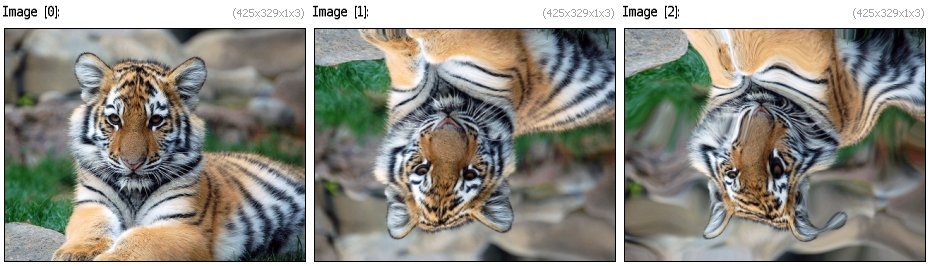
\includegraphics[keepaspectratio=true,height=7cm,width=\textwidth]{img/gmic_def1.jpg}\\
{\footnotesize \textbf{Example 1~:} \texttt{image.jpg -command "foo : -mirror y -deform \$""1" --foo[0] 5 --foo[0] 15}}
\end{center}

\subsection{\emph{-cupid\index{-cupid}} }\vspace*{-0.5em}
~\\\textbf{Arguments: } 
{\small \texttt{\_size$>$0}}\\~\\
Input cupid binary mask with specified size.
\begin{center}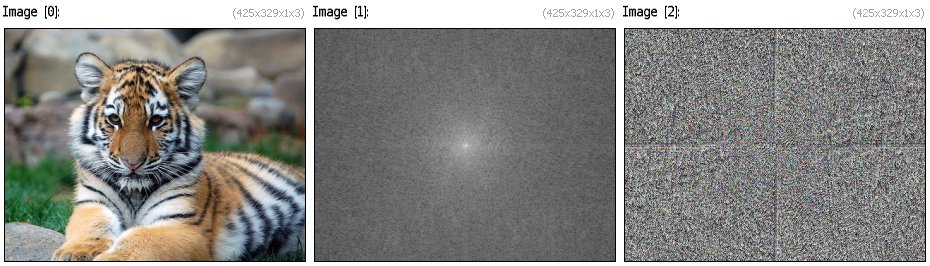
\includegraphics[keepaspectratio=true,height=7cm,width=\textwidth]{img/gmic_def2.jpg}\\
{\footnotesize \textbf{Example 2~:} \texttt{-cupid ,}}
\end{center}

\subsection{\emph{-cursor\index{-cursor}} (+)}\vspace*{-0.5em}
~\\\textbf{Arguments: } 
{\small \texttt{\_mode = \{ 0=hide ~$|$~ 1=show \}}}\\~\\
Show or hide mouse cursor for selected instant windows.
~\\Command subset (if any) stands for instant window indices instead of image indices.
~\\~\\\textbf{Default value}: {\small \texttt{'mode=1'.}}


\subsection{\emph{-display\index{-display}} (+)}\vspace*{-0.5em}
~\\\textbf{Arguments: } 
{\small \texttt{\_X,\_Y,\_Z}}\\~\\
Display selected images in an interactive viewer (use the instant window [0] if opened).
~\\Arguments 'X','Y','Z' determine the initial selection view, for 3d volumetric images.
~\\(\emph{eq. to} {\small \texttt{'-d'}}).


\subsection{\emph{-display0\index{-display0}} }\vspace*{-0.5em}
Display selected images without value normalization.
~\\(\emph{eq. to} {\small \texttt{'-d0'}}).


\subsection{\emph{-display3d\index{-display3d}} (+)}\vspace*{-0.5em}
Display selected 3d objects in an interactive viewer (use the instant window [0] if opened).
~\\(\emph{eq. to} {\small \texttt{'-d3d'}}).


\subsection{\emph{-display\_array\index{-display\_array}} }\vspace*{-0.5em}
~\\\textbf{Arguments: } 
{\small \texttt{\_width$>$0,\_height$>$0}}\\~\\
Display images in interactive windows where pixel neighborhoods can be explored.
~\\~\\\textbf{Default values}: {\small \texttt{'width=13'} and \texttt{'height=width'.}}


\subsection{\emph{-display\_fft\index{-display\_fft}} }\vspace*{-0.5em}
Display fourier transform of selected images, with centered log-module and argument.
~\\(\emph{eq. to} {\small \texttt{'-dfft'}}).
\begin{center}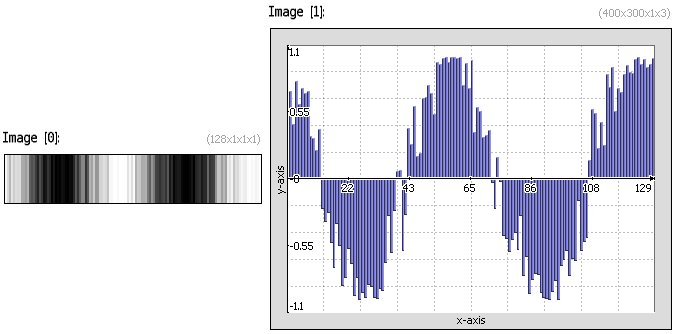
\includegraphics[keepaspectratio=true,height=7cm,width=\textwidth]{img/gmic_def3.jpg}\\
{\footnotesize \textbf{Example 3~:} \texttt{image.jpg --display\_fft}}
\end{center}

\subsection{\emph{-display\_graph\index{-display\_graph}} }\vspace*{-0.5em}
~\\\textbf{Arguments: } 
{\small \texttt{\_width$>$32,\_height$>$32,\_plot\_type,\_vertex\_type,\_xmin,\_xmax,\_ymin,\_ymax,\_xlabel,\_ylabel}}\\~\\
Render graph plot from selected image data.
~\\~\\\textbf{Default values}: {\small \texttt{'width=640', 'height=480', 'plot\_type=1', 'vertex\_type=1', 'xmin=xmax=ymin=ymax=0', 'xlabel="x-axis"'} and \texttt{'ylabel="y-axis"'.}}
\begin{center}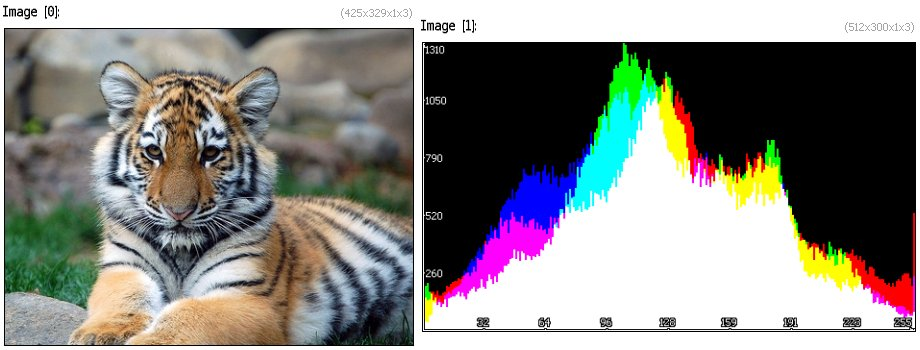
\includegraphics[keepaspectratio=true,height=7cm,width=\textwidth]{img/gmic_def4.jpg}\\
{\footnotesize \textbf{Example 4~:} \texttt{128,1,1,1,'cos(x/10+?)' --display\_graph 400,300,3}}
\end{center}

\subsection{\emph{-display\_histogram\index{-display\_histogram}} }\vspace*{-0.5em}
~\\\textbf{Arguments: } 
{\small \texttt{\_width$>$0,\_height$>$0,\_clusters$>$0,\_min\_value[\%],\_max\_value[\%],\_show\_axes=\{ 0 ~$|$~ 1 \},\_cut\_value.}}\\~\\
Render a channel-by-channel histogram.
~\\If selected image has several slices, the rendering is performed for all input slices.
~\\'cut\_value' can be \{ -1=no-cut ~$|$~ $>$=0 \}.
~\\(\emph{eq. to} {\small \texttt{'-dh'}}).
~\\~\\\textbf{Default values}: {\small \texttt{'width=512', 'height=300', 'clusters=256', 'min\_value=0\%', 'max\_value=100\%', 'show\_axes=1'} and \texttt{'cut\_value=-1'.}}
\begin{center}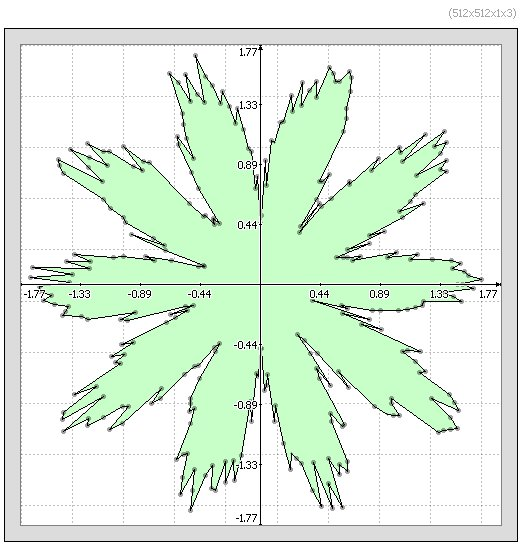
\includegraphics[keepaspectratio=true,height=7cm,width=\textwidth]{img/gmic_def5.jpg}\\
{\footnotesize \textbf{Example 5~:} \texttt{image.jpg --display\_histogram 512,300}}
\end{center}

\subsection{\emph{-display\_parametric\index{-display\_parametric}} }\vspace*{-0.5em}
~\\\textbf{Arguments: } 
{\small \texttt{\_width$>$32,\_height$>$32,\_outline\_opacity,\_vertex\_radius$>$=0,\_is\_antialiased=\{ 0 ~$|$~ 1 \},\_is\_decorated=\{ 0 ~$|$~ 1 \},\_xlabel,\_ylabel}}\\~\\
Render 2d or 3d parametric curve or point clouds from selected image data.
~\\Curve points are defined as pixels of a 2 or 3-channel image.
~\\If the point image contains more than 3 channels, additional channels define the (R,G,B) color for each vertex.
~\\If 'outline\_opacity$>$1', the outline is colored according to the specified vertex colors and 'outline\_opacity-1' is used as
the actual drawing opacity.
~\\~\\\textbf{Default values}: {\small \texttt{'width=512', 'height=width', 'outline\_opacity=3', 'vertex\_radius=0', 'is\_antialiased=1', 'is\_decorated=1', 'xlabel="x-axis"'} and \texttt{'ylabel="y-axis"'.}}
\begin{center}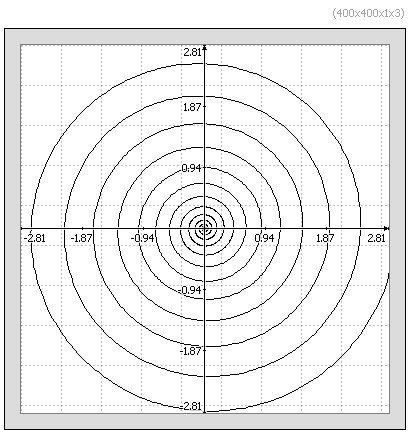
\includegraphics[keepaspectratio=true,height=7cm,width=\textwidth]{img/gmic_def6.jpg}\\
{\footnotesize \textbf{Example 6~:} \texttt{1024,1,1,2,'t=x/40;if(c==0,sin(t),cos(t))*(exp(cos(t))-2*cos(4*t)-sin(t/12)\textasciicircum 5)' -display\_parametric 512,512}}
\\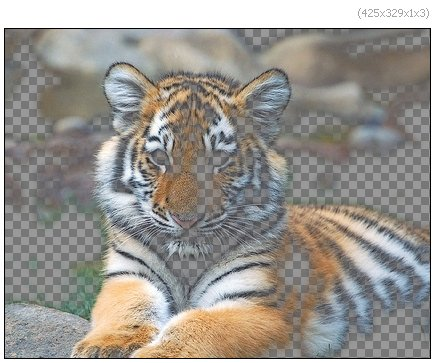
\includegraphics[keepaspectratio=true,height=7cm,width=\textwidth]{img/gmic_def7.jpg}\\
{\footnotesize \textbf{Example 7~:} \texttt{1000,1,1,2,?(-100,100) -quantize 4,1 -noise 12 -channels 0,2 --normalize 0,255 -append c -display\_parametric 512,512,0.1,8}}
\end{center}

\subsection{\emph{-display\_polar\index{-display\_polar}} }\vspace*{-0.5em}
~\\\textbf{Arguments: } 
{\small \texttt{\_width$>$32,\_height$>$32,\_outline\_type,\_fill\_R,\_fill\_G,\_fill\_B,\_theta\_start,\_theta\_end,\_xlabel,\_ylabel}}\\~\\
Render polar curve from selected image data.
~\\(\emph{eq. to} {\small \texttt{'-dp'}}).
~\\'outline\_type' can be \{ r$<$0=dots with radius -r ~$|$~ 0=no outline ~$|$~ r$>$0=lines+dots with radius r \}.
~\\'fill\_color' can be \{ -1=no fill ~$|$~ R,G,B=fill with specified color \}.
~\\~\\\textbf{Default values}: {\small \texttt{'width=500', 'height=width', 'outline\_type=1', 'fill\_R=fill\_G=fill\_B=200', 'theta\_start=0', 'theta\_end=360', 'xlabel="x-axis"'} and \texttt{'ylabel="y-axis"'.}}
\begin{center}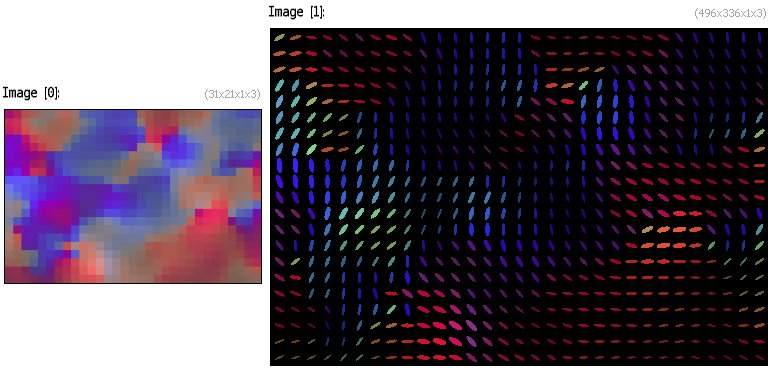
\includegraphics[keepaspectratio=true,height=7cm,width=\textwidth]{img/gmic_def8.jpg}\\
{\footnotesize \textbf{Example 8~:} \texttt{300,1,1,1,'0.3+abs(cos(10*pi*x/w))+?(0.4)' -display\_polar 512,512,4,200,255,200}}
\\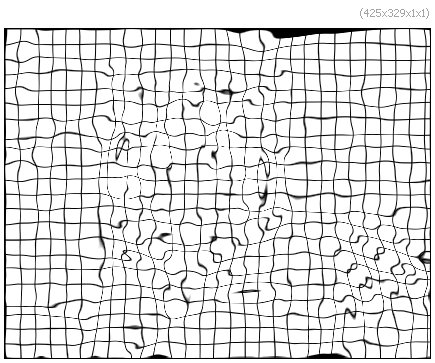
\includegraphics[keepaspectratio=true,height=7cm,width=\textwidth]{img/gmic_def9.jpg}\\
{\footnotesize \textbf{Example 9~:} \texttt{3000,1,1,1,'x\textasciicircum 3/1e10' -display\_polar 400,400,1,-1,,,0,\{15*360\}}}
\end{center}

\subsection{\emph{-display\_rgba\index{-display\_rgba}} }\vspace*{-0.5em}
Render selected RGBA images over a checkerboard background.
~\\(\emph{eq. to} {\small \texttt{'-drgba'}}).
\begin{center}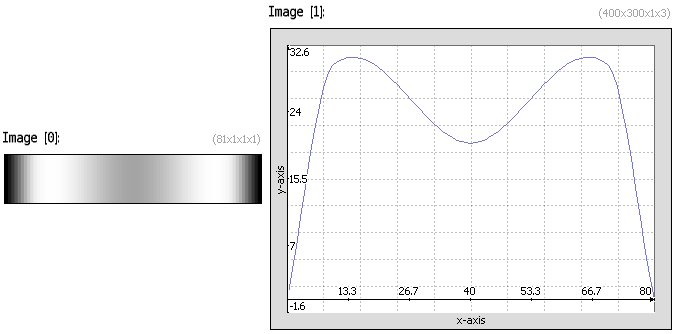
\includegraphics[keepaspectratio=true,height=7cm,width=\textwidth]{img/gmic_def10.jpg}\\
{\footnotesize \textbf{Example 10~:} \texttt{image.jpg --norm -threshold[-1] 40\% -blur[-1] 3 -normalize[-1] 0,255 -append c -display\_rgba}}
\end{center}

\subsection{\emph{-display\_tensors\index{-display\_tensors}} }\vspace*{-0.5em}
~\\\textbf{Arguments: } 
{\small \texttt{\_size\_factor$>$0,\_ellipse\_factor$>$=0,\_colored\_mode=\{ 0 ~$|$~ 1 \}}}\\~\\
Render selected mask field of 2x2 tensors with ellipses.
~\\(\emph{eq. to} {\small \texttt{'-dt'}}).
~\\~\\\textbf{Default values}: {\small \texttt{'size\_factor=16', 'ellipse\_factor=0.92', 'color\_mode=1'.}}
\begin{center}
\includegraphics[keepaspectratio=true,height=7cm,width=\textwidth]{img/gmic_def11.jpg}\\
{\footnotesize \textbf{Example 11~:} \texttt{image.jpg -diffusiontensors 0.7,0.6 -crop 60,10,90,30 --display\_tensors ,}}
\end{center}

\subsection{\emph{-display\_warp\index{-display\_warp}} }\vspace*{-0.5em}
~\\\textbf{Arguments: } 
{\small \texttt{\_cell\_size$>$0}}\\~\\
Render selected 2d warping fields.
~\\(\emph{eq. to} {\small \texttt{'-dw'}}).
~\\~\\\textbf{Default value}: {\small \texttt{'cell\_size=15'.}}
\begin{center}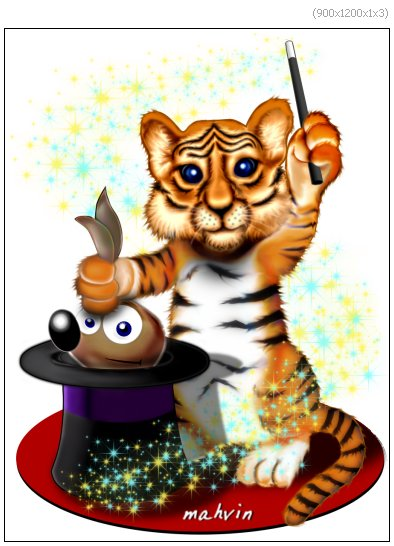
\includegraphics[keepaspectratio=true,height=7cm,width=\textwidth]{img/gmic_def12.jpg}\\
{\footnotesize \textbf{Example 12~:} \texttt{image.jpg -luminance -blur 5 -gradient -append c -display\_warp ,}}
\end{center}

\subsection{\emph{-document\_gmic\index{-document\_gmic}} }\vspace*{-0.5em}
~\\\textbf{Arguments: } 
{\small \texttt{\_format=\{ ascii ~$|$~ html ~$|$~ latex ~$|$~ xml ~$|$~ bash ~$|$~ images \},\_image\_path,\_write\_wrapper=\{ 0 ~$|$~ 1 \}}}\\~\\
Create documentation of .gmic command files (loaded as raw 'uchar' images), in specified format.
~\\~\\\textbf{Default values}: {\small \texttt{'format=ascii', 'image\_path=""'} and \texttt{'write\_wrapper=1'.\textbackslash n}}
~\\Example(s) : raw:file.gmic,uchar -document\_gmic html,img


\subsection{\emph{-echo\index{-echo}} (*)}\vspace*{-0.5em}
~\\\textbf{Arguments: } 
{\small \texttt{message}}\\~\\
Output specified message, on the error output.
~\\(\emph{eq. to} {\small \texttt{'-e'}}).
~\\Command subset (if any) stands for displayed scope indices instead of image indices.


\subsection{\emph{-echo\_file\index{-echo\_file}} }\vspace*{-0.5em}
~\\\textbf{Arguments: } 
{\small \texttt{filename,message}}\\~\\
Output specified message, appending it to specified output file.
~\\(similar to '-echo' for specified output file stream).


\subsection{\emph{-echo\_stdout\index{-echo\_stdout}} }\vspace*{-0.5em}
~\\\textbf{Arguments: } 
{\small \texttt{message}}\\~\\
Output specified message, on the standard output (stdout).
~\\(similar to '-echo' for output on standard output instead of standard error).


\subsection{\emph{-function1d\index{-function1d}} }\vspace*{-0.5em}
~\\\textbf{Arguments: } 
{\small \texttt{0$<$=smoothness$<$=1,x0$>$=0,y0,x1$>$=0,y1,...,xn$>$=0,yn}}\\~\\
Input continuous 1d function from specified list of keypoints (xk,yk)
in range [0,max(xk)] (xk are positive integers).
~\\~\\\textbf{Default values}: {\small \texttt{'smoothness=1'} and \texttt{'x0=y0=0'.}}
\begin{center}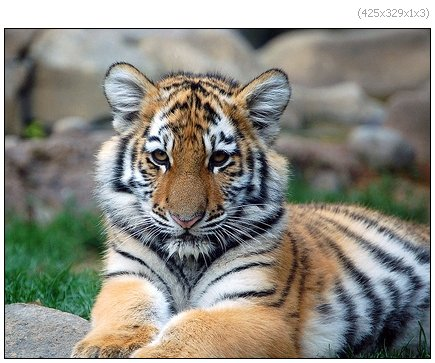
\includegraphics[keepaspectratio=true,height=7cm,width=\textwidth]{img/gmic_def13.jpg}\\
{\footnotesize \textbf{Example 13~:} \texttt{-function1d 1,0,0,10,30,40,20,70,30,80,0 --display\_graph 400,300}}
\end{center}

\subsection{\emph{-gmicky\index{-gmicky}} }\vspace*{-0.5em}
Load a new image of the G'MIC mascot 'Gmicky'.
\begin{center}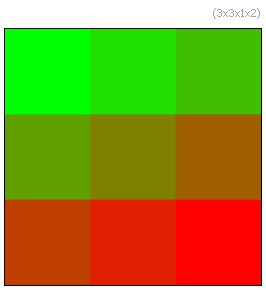
\includegraphics[keepaspectratio=true,height=7cm,width=\textwidth]{img/gmic_def14.jpg}\\
{\footnotesize \textbf{Example 14~:} \texttt{-gmicky}}
\end{center}

\subsection{\emph{-gmicky\_wilber\index{-gmicky\_wilber}} }\vspace*{-0.5em}
Load a new image of the G'MIC mascot 'Gmicky' together with GIMP mascot 'Wilber'.
\begin{center}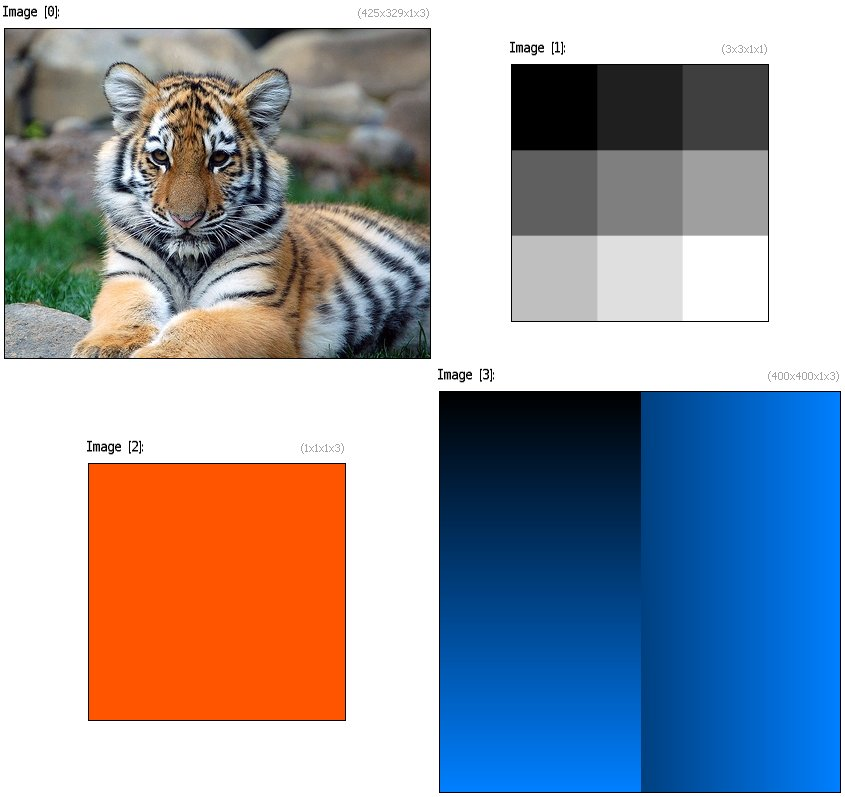
\includegraphics[keepaspectratio=true,height=7cm,width=\textwidth]{img/gmic_def15.jpg}\\
{\footnotesize \textbf{Example 15~:} \texttt{-gmicky\_wilber}}
\end{center}

\subsection{\emph{-heart\index{-heart}} }\vspace*{-0.5em}
~\\\textbf{Arguments: } 
{\small \texttt{\_width$>$0,\_height$>$0}}\\~\\
Input heart binary mask with specified size.
\begin{center}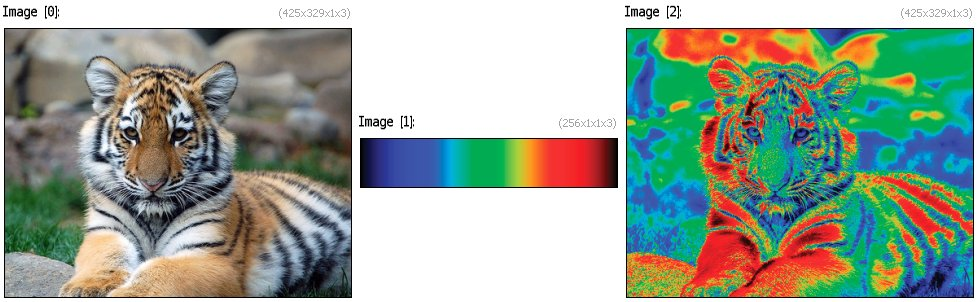
\includegraphics[keepaspectratio=true,height=7cm,width=\textwidth]{img/gmic_def16.jpg}\\
{\footnotesize \textbf{Example 16~:} \texttt{-heart ,}}
\end{center}

\subsection{\emph{-input\index{-input}} (*)}\vspace*{-0.5em}
~\\\textbf{Arguments: } 
{\small \texttt{[type:]filename}}~~~$|$\\
\hspace*{2.2cm}{\small \texttt{[type:]http://URL}}~~~$|$\\
\hspace*{2.2cm}{\small \texttt{[selection]x\_nb\_copies$>$0}}~~~$|$\\
\hspace*{2.2cm}{\small \texttt{\{ width$>$0[\%] ~$|$~ [image\_w] \},\{ \_height$>$0[\%] ~$|$~ [image\_h] \},\{ \_depth$>$0[\%] ~$|$~ [image\_d] \},\{ \_spectrum$>$0[\%] ~$|$~ [image\_s] \},\_\{ value1,\_value2,.. ~$|$~ 'formula' \}}}~~~$|$\\
\hspace*{2.2cm}{\small \texttt{(value1\{,~$|$~;~$|$~/~$|$~\textasciicircum \}value2\{,~$|$~;~$|$~/~$|$~\textasciicircum \}..)}}~~~$|$\\
\hspace*{2.2cm}{\small \texttt{0}}\\~\\
Insert a new image taken from a filename or from a copy of an existing image ['indice'],"
or insert new image with specified dimensions and values. Single quotes may be omitted in
~\\'formula'. Specifying argument '0' inserts an 'empty' image.
~\\(\emph{eq. to} {\small \texttt{'-i' ~$|$~ (no args}}).
~\\~\\\textbf{Default values}: {\small \texttt{'nb\_copies=1', 'height=depth=spectrum=1'} and \texttt{'value1=0'.}}
\begin{center}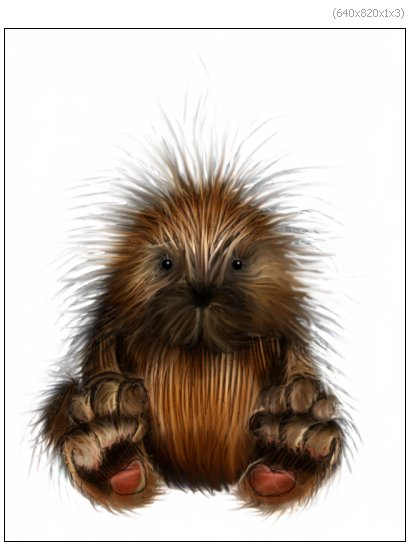
\includegraphics[keepaspectratio=true,height=7cm,width=\textwidth]{img/gmic_def17.jpg}\\
{\footnotesize \textbf{Example 17~:} \texttt{-input image.jpg}}
\\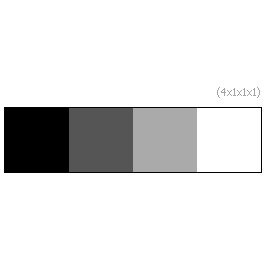
\includegraphics[keepaspectratio=true,height=7cm,width=\textwidth]{img/gmic_def18.jpg}\\
{\footnotesize \textbf{Example 18~:} \texttt{-i (1,2,3;4,5,6;7,8,9\textasciicircum 9,8,7;6,5,4;3,2,1)}}
\\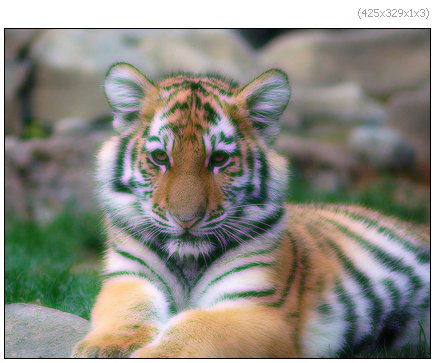
\includegraphics[keepaspectratio=true,height=7cm,width=\textwidth]{img/gmic_def19.jpg}\\
{\footnotesize \textbf{Example 19~:} \texttt{image.jpg (1,2,3;4,5,6;7,8,9) (255\textasciicircum 128\textasciicircum 64) 400,400,1,3,'if(x$>$w/2,x,y)*c'}}
\end{center}

\subsection{\emph{-output\index{-output}} (*)}\vspace*{-0.5em}
~\\\textbf{Arguments: } 
{\small \texttt{[type:]filename,\_format\_options}}\\~\\
Output selected images as one or several numbered file(s).
~\\(\emph{eq. to} {\small \texttt{'-o'}}).
~\\~\\\textbf{Default value}: {\small \texttt{'format\_options'=(undefined).}}


\subsection{\emph{-output\_ggr\index{-output\_ggr}} }\vspace*{-0.5em}
~\\\textbf{Arguments: } 
{\small \texttt{filename,\_gradient\_name}}\\~\\
Output selected images as GIMP gradient files.
~\\If no gradient name is specified, it is deduced from the filename.


\subsection{\emph{-outputn\index{-outputn}} }\vspace*{-0.5em}
~\\\textbf{Arguments: } 
{\small \texttt{filename}}\\~\\
Output selected images as automatically numbered filenames in repeat..done loops.
~\\(\emph{eq. to} {\small \texttt{'-on'}}).


\subsection{\emph{-outputp\index{-outputp}} }\vspace*{-0.5em}
~\\\textbf{Arguments: } 
{\small \texttt{prefix}}\\~\\
Output selected images as prefixed versions of their original filenames.
~\\(\emph{eq. to} {\small \texttt{'-op'}}).
~\\~\\\textbf{Default value}: {\small \texttt{'prefix=\_'.}}


\subsection{\emph{-outputw\index{-outputw}} }\vspace*{-0.5em}
Output selected images by overwritting their original location.
~\\(\emph{eq. to} {\small \texttt{'-ow'}}).


\subsection{\emph{-plot\index{-plot}} (+)}\vspace*{-0.5em}
~\\\textbf{Arguments: } 
{\small \texttt{\_plot\_type,\_vertex\_type,\_xmin,\_xmax,\_ymin,\_ymax}}~~~$|$\\
\hspace*{2.2cm}{\small \texttt{'formula',\_resolution$>$=0,\_plot\_type,\_vertex\_type,\_xmin,xmax,\_ymin,\_ymax}}\\~\\
Display selected image or formula in an interactive viewer (use the instant window [0] if opened).
~\\'plot\_type' can be \{ 0=none ~$|$~ 1=lines ~$|$~ 2=splines ~$|$~ 3=bar \}.
~\\'vertex\_type' can be \{ 0=none ~$|$~ 1=points ~$|$~ 2,3=crosses ~$|$~ 4,5=circles ~$|$~ 6,7=squares \}.
~\\'xmin','xmax','ymin','ymax' set the coordinates of the displayed xy-axes.
~\\~\\\textbf{Default values}: {\small \texttt{'plot\_type=1', 'vertex\_type=1'} and \texttt{'xmin=xmax=ymin=ymax=0 (auto)'.}}


\subsection{\emph{-print\index{-print}} (*)}\vspace*{-0.5em}
Output information on selected images, on the standard error (stderr).
~\\(\emph{eq. to} {\small \texttt{'-p'}}).


\subsection{\emph{-rainbow\_lut\index{-rainbow\_lut}} }\vspace*{-0.5em}
Input a 256-entries RGB colormap of rainbow colors.
\begin{center}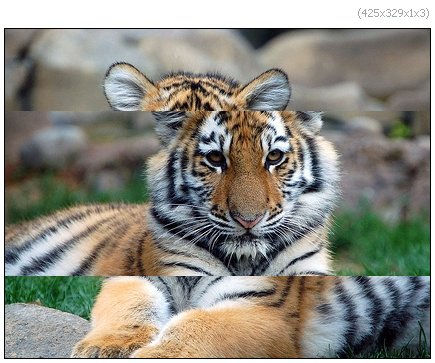
\includegraphics[keepaspectratio=true,height=7cm,width=\textwidth]{img/gmic_def20.jpg}\\
{\footnotesize \textbf{Example 20~:} \texttt{image.jpg -rainbow\_lut --luminance[-2] -map[-1] [-2]}}
\end{center}

\subsection{\emph{-roddy\index{-roddy}} }\vspace*{-0.5em}
Load a new image of the G'MIC Rodilius mascot 'Roddy'.
\begin{center}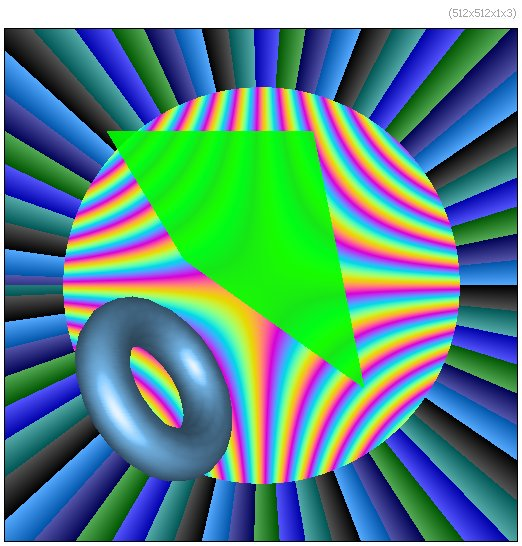
\includegraphics[keepaspectratio=true,height=7cm,width=\textwidth]{img/gmic_def21.jpg}\\
{\footnotesize \textbf{Example 21~:} \texttt{-roddy}}
\end{center}

\subsection{\emph{-remove\_duplicates\index{-remove\_duplicates}} }\vspace*{-0.5em}
Remove duplicates images in the selected images list.
\begin{center}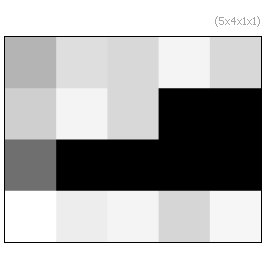
\includegraphics[keepaspectratio=true,height=7cm,width=\textwidth]{img/gmic_def22.jpg}\\
{\footnotesize \textbf{Example 22~:} \texttt{(1,2,3,4,2,4,3,1,3,4,2,1) -split x -remove\_duplicates -append x}}
\end{center}

\subsection{\emph{-remove\_empty\index{-remove\_empty}} }\vspace*{-0.5em}
Remove empty images in the selected image list.


\subsection{\emph{-select\index{-select}} (+)}\vspace*{-0.5em}
~\\\textbf{Arguments: } 
{\small \texttt{feature\_type,\_X,\_Y,\_Z}}\\~\\
Interactively select a feature from selected images (use the instant window [0] if opened).
~\\'feature\_type' can be \{ 0=point ~$|$~ 1=segment ~$|$~ 2=rectangle ~$|$~ 3=ellipse \}.
~\\Arguments 'X','Y','Z' determine the initial selection view, for 3d volumetric images.
~\\The retrieved feature is returned as a 3d or 6d vector containing the feature coordinates.


\subsection{\emph{-shared\index{-shared}} (*)}\vspace*{-0.5em}
~\\\textbf{Arguments: } 
{\small \texttt{x0[\%],x1[\%],y[\%],z[\%],v[\%]}}~~~$|$\\
\hspace*{2.2cm}{\small \texttt{y0[\%],y1[\%],z[\%],v[\%]}}~~~$|$\\
\hspace*{2.2cm}{\small \texttt{z0[\%],z1[\%],v[\%]}}~~~$|$\\
\hspace*{2.2cm}{\small \texttt{v0[\%],v1[\%]}}~~~$|$\\
\hspace*{2.2cm}{\small \texttt{(no args)}}\\~\\
Insert shared buffers from (opt. points/rows/planes/channels of) selected images.
~\\(\emph{eq. to} {\small \texttt{'-sh'}}).
\begin{center}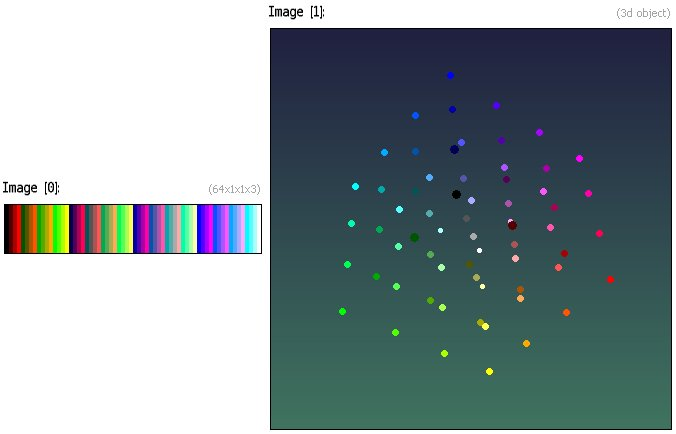
\includegraphics[keepaspectratio=true,height=7cm,width=\textwidth]{img/gmic_def23.jpg}\\
{\footnotesize \textbf{Example 23~:} \texttt{image.jpg -shared 1,1 -blur[-1] 3 -remove[-1]}}
\\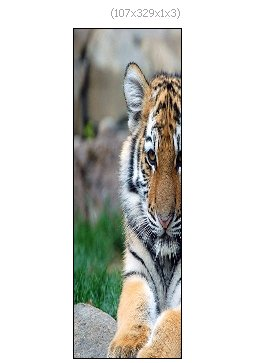
\includegraphics[keepaspectratio=true,height=7cm,width=\textwidth]{img/gmic_def24.jpg}\\
{\footnotesize \textbf{Example 24~:} \texttt{image.jpg -repeat \{s\} -shared 25\%,75\%,0,\$$>$ -mirror[-1] x -remove[-1] -done}}
\end{center}

\subsection{\emph{-srand\index{-srand}} (*)}\vspace*{-0.5em}
~\\\textbf{Arguments: } 
{\small \texttt{value}}~~~$|$\\
\hspace*{2.2cm}{\small \texttt{(no args)}}\\~\\
Set random generator seed.
~\\If no argument is specified, a random value is used as the random generator seed.


\subsection{\emph{-testimage2d\index{-testimage2d}} }\vspace*{-0.5em}
~\\\textbf{Arguments: } 
{\small \texttt{\_width$>$0,\_height$>$0,\_spectrum$>$0}}\\~\\
Input a 2d synthetic image.
~\\~\\\textbf{Default values}: {\small \texttt{'width=512', 'height=width'} and \texttt{'spectrum=3'.}}
\begin{center}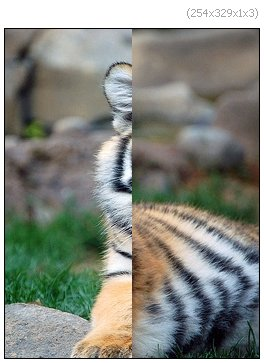
\includegraphics[keepaspectratio=true,height=7cm,width=\textwidth]{img/gmic_def25.jpg}\\
{\footnotesize \textbf{Example 25~:} \texttt{-testimage2d 512}}
\end{center}

\subsection{\emph{-text2img\index{-text2img}} }\vspace*{-0.5em}
~\\\textbf{Arguments: } 
{\small \texttt{text,\_line\_separator}}\\~\\
Input a 2d image whose values are ASCII characters of specified input text.
~\\~\\\textbf{Default value}: {\small \texttt{'line\_separator= '.}}
\begin{center}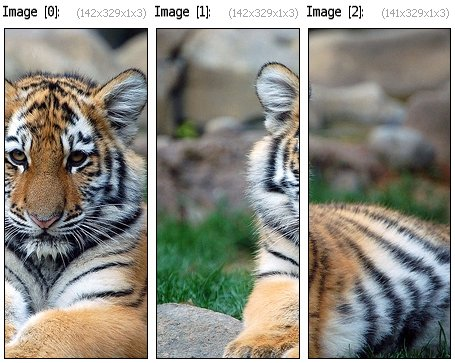
\includegraphics[keepaspectratio=true,height=7cm,width=\textwidth]{img/gmic_def26.jpg}\\
{\footnotesize \textbf{Example 26~:} \texttt{-text2img "There are 4 words"}}
\end{center}

\subsection{\emph{-type\index{-type}} (*)}\vspace*{-0.5em}
~\\\textbf{Arguments: } 
{\small \texttt{datatype}}\\~\\
Set pixel datatype for all images of the list.
~\\'datatype' can be \{ bool ~$|$~ uchar ~$|$~ char ~$|$~ ushort ~$|$~ short ~$|$~ uint ~$|$~ int ~$|$~ float ~$|$~ double \}.
~\\Depending on how your G'MIC version has been compiled, some datatypes may be unavailable
~\\(typically datatypes different from 'float').


\subsection{\emph{-uncommand\index{-uncommand}} (*)}\vspace*{-0.5em}
~\\\textbf{Arguments: } 
{\small \texttt{command\_name}}~~~$|$\\
\hspace*{2.2cm}{\small \texttt{*}}\\~\\
Discard last definition of specified custom command.
~\\Set argument to '*' for discarding all existing custom commands.


\subsection{\emph{-uniform\_distribution\index{-uniform\_distribution}} }\vspace*{-0.5em}
~\\\textbf{Arguments: } 
{\small \texttt{nb\_levels$>$=1,spectrum$>$=1}}\\~\\
Input set of uniformly distributed N-d points in [0,1]\textasciicircum N.
\begin{center}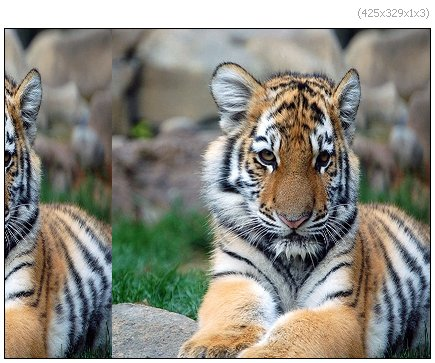
\includegraphics[keepaspectratio=true,height=7cm,width=\textwidth]{img/gmic_def27.jpg}\\
{\footnotesize \textbf{Example 27~:} \texttt{-uniform\_distribution 64,3 -* 255 --distribution3d -circles3d[-1] 10}}
\end{center}

\subsection{\emph{-update\index{-update}} }\vspace*{-0.5em}
Update commands from the latest definition file on the G'MIC server.
~\\This requires an active Internet connection and an access to the external
tools 'curl' or 'wget'.
~\\(\emph{eq. to} {\small \texttt{'-up'}}).


\subsection{\emph{-verbose\index{-verbose}} (*)}\vspace*{-0.5em}
~\\\textbf{Arguments: } 
{\small \texttt{\_level}}~~~$|$\\
\hspace*{2.2cm}{\small \texttt{\{ + ~$|$~ - \}}}\\~\\
Set or increment/decrement the verbosity level.
~\\(\emph{eq. to} {\small \texttt{'-v'}}).
~\\When 'level'$>$=0, G'MIC log messages are displayed on the standard error (stderr).
~\\~\\\textbf{Default value}: {\small \texttt{'level=0'.}}


\subsection{\emph{-wait\index{-wait}} (+)}\vspace*{-0.5em}
~\\\textbf{Arguments: } 
{\small \texttt{delay}}~~~$|$\\
\hspace*{2.2cm}{\small \texttt{(no args)}}\\~\\
Wait for a given delay (in ms) since last call, or sleep during a specified delay,
or wait for a user event occuring on the selected instant window.
~\\'delay' can be \{ $<$0=delay+flush ~$|$~ 0=event ~$|$~ $>$0=delay \}.
~\\Command subset (if any) stands for instant window indices instead of image indices.
~\\If no window indices are specified and if 'delay' is negative, the command results
in a hard sleep during specified delay.
~\\~\\\textbf{Default value}: {\small \texttt{'delay=0'.}}


\subsection{\emph{-warn\index{-warn}} (*)}\vspace*{-0.5em}
~\\\textbf{Arguments: } 
{\small \texttt{message}}\\~\\
Print specified warning message, on the standard error (stderr).
~\\Command subset (if any) stands for displayed scope indices instead of image indices.


\subsection{\emph{-window\index{-window}} (+)}\vspace*{-0.5em}
~\\\textbf{Arguments: } 
{\small \texttt{\_width[\%]$>$=-1,\_height[\%]$>$=-1,\_normalization,\_fullscreen,\_pos\_x[\%],\_pos\_y[\%],\_title}}\\~\\
Display selected images into an instant window with specified size, normalization type,
fullscreen mode and title.
~\\(\emph{eq. to} {\small \texttt{'-w'}}).
~\\If 'width' or 'height' is set to -1, the corresponding dimension is adjusted to the window
or image size.
~\\When arguments 'pos\_x' and 'pos\_y' are both different than -1, the window is moved to
the specified coordinates.
~\\'width'=0 or 'height'=0 closes the instant window.
~\\'normalization' can be \{ -1=keep same ~$|$~ 0=none ~$|$~ 1=always ~$|$~ 2=1st-time ~$|$~ 3=auto \}.
~\\'fullscreen' can be \{ -1=keep same ~$|$~ 0=no ~$|$~ 1=yes \}.
~\\You can manage up to 10 different instant windows by using the numbered variants
~\\'-w0' (default, eq. to '-w'),'-w1',..,'-w9' of the command '-w'.
~\\~\\\textbf{Default values}: {\small \texttt{'width=height=normalization=fullscreen=-1'} and \texttt{'title=(undefined)'.}}

\section{List manipulation}


\subsection{\emph{-keep\index{-keep}} (*)}\vspace*{-0.5em}
Keep only selected images.
~\\(\emph{eq. to} {\small \texttt{'-k'}}).
\begin{center}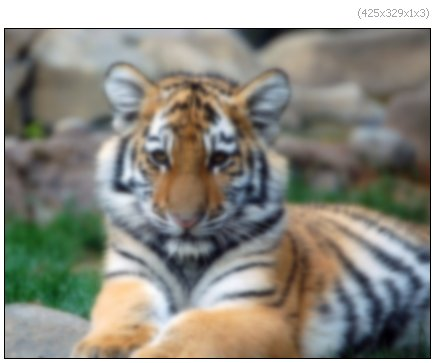
\includegraphics[keepaspectratio=true,height=7cm,width=\textwidth]{img/gmic_def28.jpg}\\
{\footnotesize \textbf{Example 28~:} \texttt{image.jpg -split x -keep[0-50\%:2] -append x}}
\\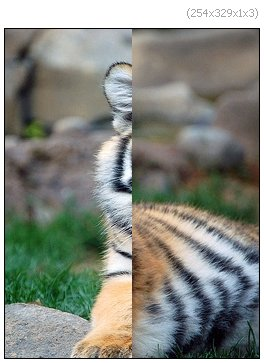
\includegraphics[keepaspectratio=true,height=7cm,width=\textwidth]{img/gmic_def29.jpg}\\
{\footnotesize \textbf{Example 29~:} \texttt{image.jpg -split x -keep[\textasciicircum 30\%-70\%] -append x}}
\end{center}

\subsection{\emph{-move\index{-move}} (*)}\vspace*{-0.5em}
~\\\textbf{Arguments: } 
{\small \texttt{position[\%]}}\\~\\
Move selected images at specified position.
~\\(\emph{eq. to} {\small \texttt{'-mv'}}).
\begin{center}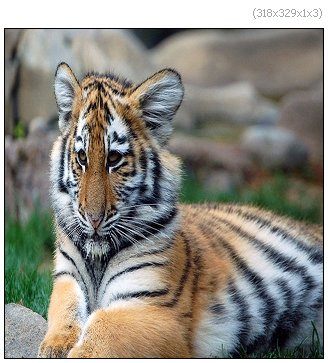
\includegraphics[keepaspectratio=true,height=7cm,width=\textwidth]{img/gmic_def30.jpg}\\
{\footnotesize \textbf{Example 30~:} \texttt{image.jpg -split x,3 -move[1] 0}}
\\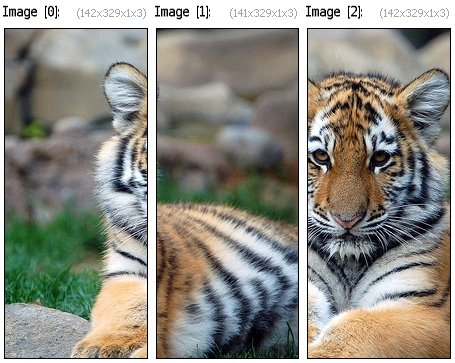
\includegraphics[keepaspectratio=true,height=7cm,width=\textwidth]{img/gmic_def31.jpg}\\
{\footnotesize \textbf{Example 31~:} \texttt{image.jpg -split x -move[50\%--1:2] 0 -append x}}
\end{center}

\subsection{\emph{-name\index{-name}} (*)}\vspace*{-0.5em}
~\\\textbf{Arguments: } 
{\small \texttt{name,\_is\_modified=\{ 0 ~$|$~ 1 \}}}\\~\\
Set name of selected images.
~\\(\emph{eq. to} {\small \texttt{'-nm'}}).
~\\Argument 'is\_modified' tells about the modified state of selected images.
~\\~\\\textbf{Default value}: {\small \texttt{'is\_modified=0'.}}
\begin{center}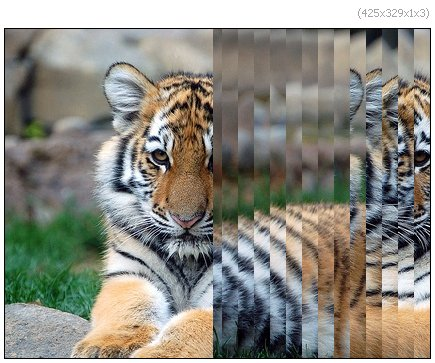
\includegraphics[keepaspectratio=true,height=7cm,width=\textwidth]{img/gmic_def32.jpg}\\
{\footnotesize \textbf{Example 32~:} \texttt{image.jpg -name image -blur[image] 2}}
\end{center}

\subsection{\emph{-remove\index{-remove}} (*)}\vspace*{-0.5em}
Remove selected images.
~\\(\emph{eq. to} {\small \texttt{'-rm'}}).
\begin{center}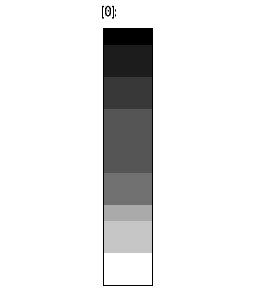
\includegraphics[keepaspectratio=true,height=7cm,width=\textwidth]{img/gmic_def33.jpg}\\
{\footnotesize \textbf{Example 33~:} \texttt{image.jpg -split x -remove[30\%-70\%] -append x}}
\\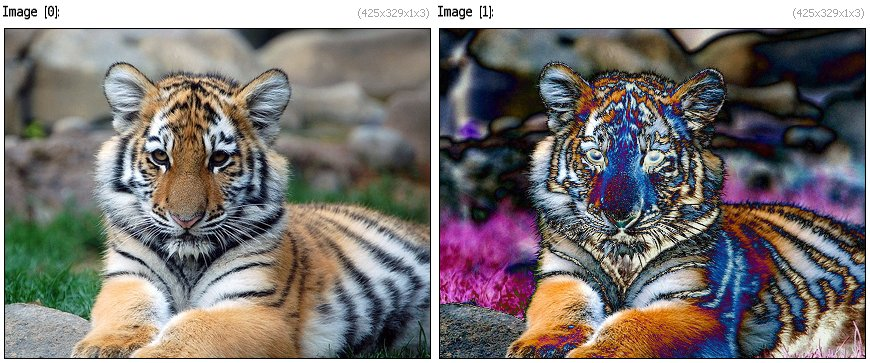
\includegraphics[keepaspectratio=true,height=7cm,width=\textwidth]{img/gmic_def34.jpg}\\
{\footnotesize \textbf{Example 34~:} \texttt{image.jpg -split x -remove[0-50\%:2] -append x}}
\end{center}

\subsection{\emph{-reverse\index{-reverse}} (*)}\vspace*{-0.5em}
Reverse positions of selected images.
~\\(\emph{eq. to} {\small \texttt{'-rv'}}).
\begin{center}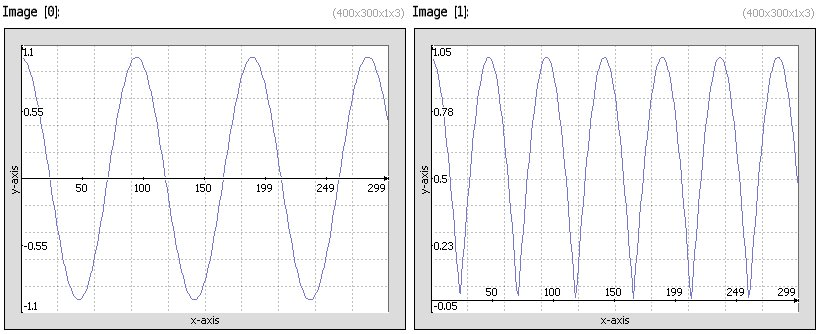
\includegraphics[keepaspectratio=true,height=7cm,width=\textwidth]{img/gmic_def35.jpg}\\
{\footnotesize \textbf{Example 35~:} \texttt{image.jpg -split x,3 -reverse[-2,-1]}}
\\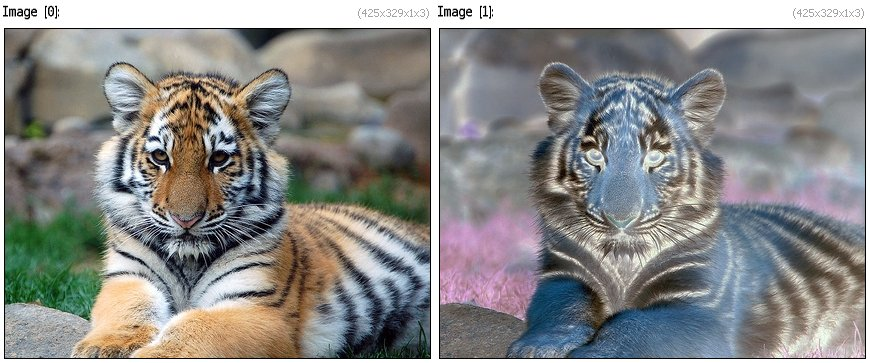
\includegraphics[keepaspectratio=true,height=7cm,width=\textwidth]{img/gmic_def36.jpg}\\
{\footnotesize \textbf{Example 36~:} \texttt{image.jpg -split x,-16 -reverse[50\%-100\%] -append x}}
\end{center}

\subsection{\emph{-sort\_list\index{-sort\_list}} }\vspace*{-0.5em}
~\\\textbf{Arguments: } 
{\small \texttt{\_ordering=\{ + ~$|$~ - \},\_criterion}}\\~\\
Sort list of selected images according to the specified image criterion.
~\\~\\\textbf{Default values}: {\small \texttt{'ordering=+', 'criterion=i'.}}
\begin{center}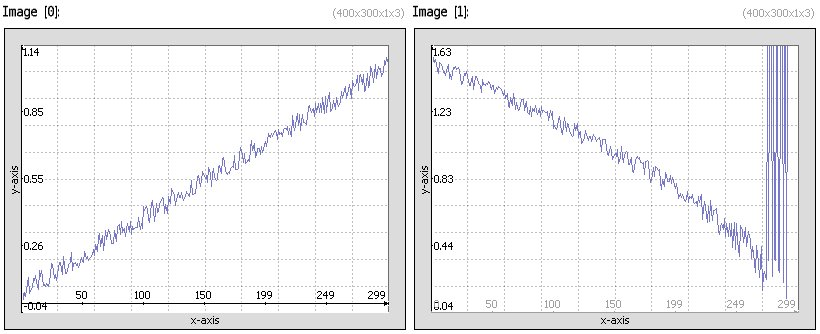
\includegraphics[keepaspectratio=true,height=7cm,width=\textwidth]{img/gmic_def37.jpg}\\
{\footnotesize \textbf{Example 37~:} \texttt{(1;4;7;3;9;2;4;7;6;3;9;1;0;3;3;2) -split y -sort\_list + -append y}}
\end{center}

\subsection{\emph{-sort\_str\index{-sort\_str}} }\vspace*{-0.5em}
Sort selected images (viewed as a list of strings) in lexicographic order.

\section{Mathematical operators}


\subsection{\emph{-abs\index{-abs}} (+)}\vspace*{-0.5em}
Compute the pointwise absolute values of selected images.
\begin{center}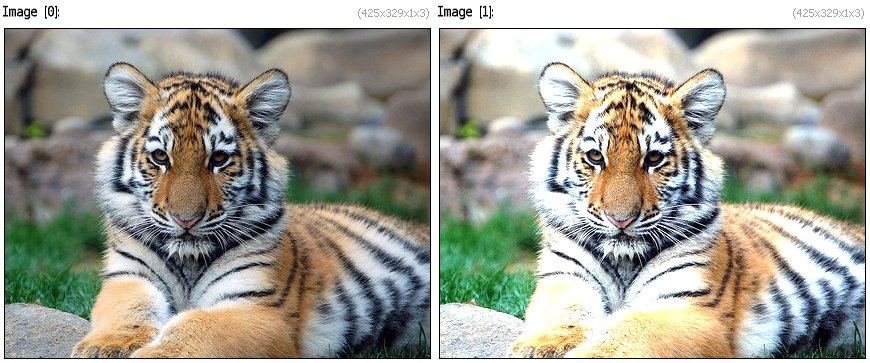
\includegraphics[keepaspectratio=true,height=7cm,width=\textwidth]{img/gmic_def38.jpg}\\
{\footnotesize \textbf{Example 38~:} \texttt{image.jpg --sub \{ia\} -abs[-1]}}
\\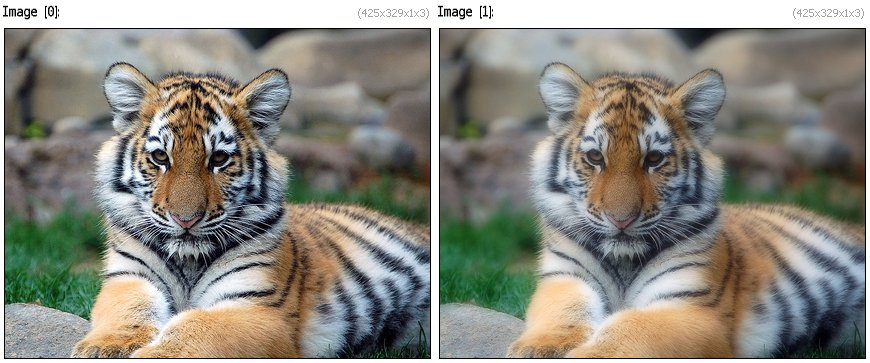
\includegraphics[keepaspectratio=true,height=7cm,width=\textwidth]{img/gmic_def39.jpg}\\
{\footnotesize \textbf{Example 39~:} \texttt{300,1,1,1,'cos(20*x/w)' --abs -display\_graph 400,300}}
\end{center}

\subsection{\emph{-acos\index{-acos}} (+)}\vspace*{-0.5em}
Compute the pointwise arc-cosine of selected images.
\begin{center}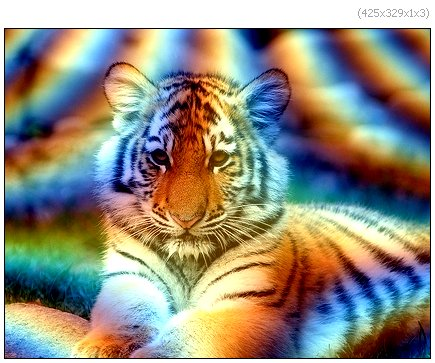
\includegraphics[keepaspectratio=true,height=7cm,width=\textwidth]{img/gmic_def40.jpg}\\
{\footnotesize \textbf{Example 40~:} \texttt{image.jpg --normalize -1,1 -acos[-1]}}
\\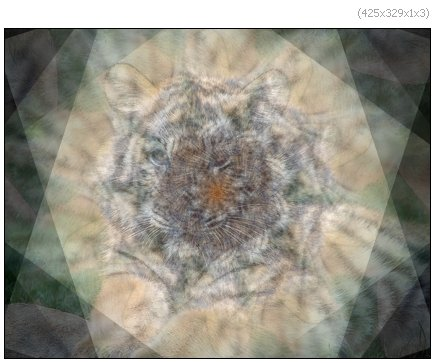
\includegraphics[keepaspectratio=true,height=7cm,width=\textwidth]{img/gmic_def41.jpg}\\
{\footnotesize \textbf{Example 41~:} \texttt{300,1,1,1,'x/w+0.1*u' --acos -display\_graph 400,300}}
\end{center}

\subsection{\emph{-add\index{-add}} (+)}\vspace*{-0.5em}
~\\\textbf{Arguments: } 
{\small \texttt{value[\%]}}~~~$|$\\
\hspace*{2.2cm}{\small \texttt{[image]}}~~~$|$\\
\hspace*{2.2cm}{\small \texttt{'formula'}}~~~$|$\\
\hspace*{2.2cm}{\small \texttt{(no args)}}\\~\\
Add specified value, image or mathematical expression to selected images,
or compute the pointwise sum of selected images.
~\\(\emph{eq. to} {\small \texttt{'-+'}}).
\begin{center}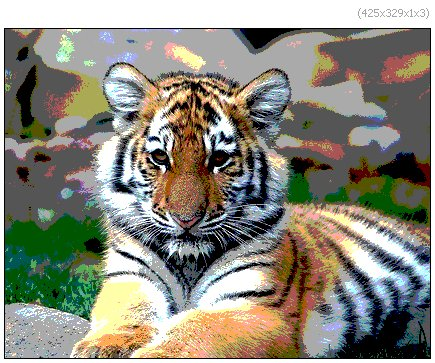
\includegraphics[keepaspectratio=true,height=7cm,width=\textwidth]{img/gmic_def42.jpg}\\
{\footnotesize \textbf{Example 42~:} \texttt{image.jpg --add 30\% -cut 0,255}}
\\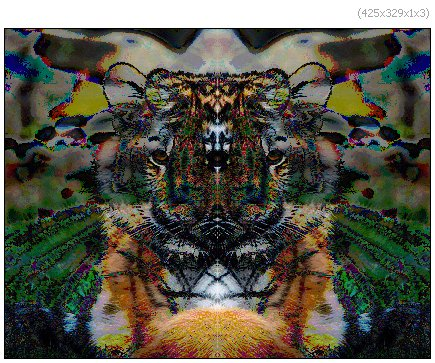
\includegraphics[keepaspectratio=true,height=7cm,width=\textwidth]{img/gmic_def43.jpg}\\
{\footnotesize \textbf{Example 43~:} \texttt{image.jpg --blur 5 -normalize 0,255 -add[1] [0]}}
\\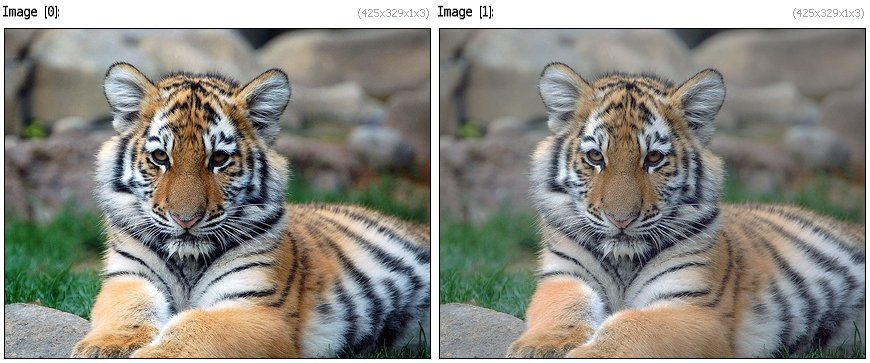
\includegraphics[keepaspectratio=true,height=7cm,width=\textwidth]{img/gmic_def44.jpg}\\
{\footnotesize \textbf{Example 44~:} \texttt{image.jpg -add '80*cos(80*(x/w-0.5)*(y/w-0.5)+c)' -cut 0,255}}
\\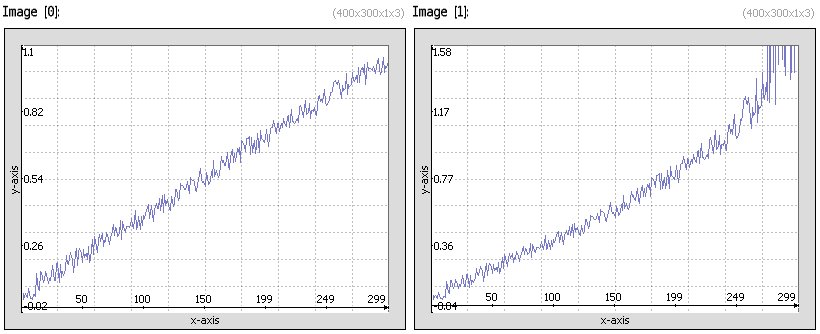
\includegraphics[keepaspectratio=true,height=7cm,width=\textwidth]{img/gmic_def45.jpg}\\
{\footnotesize \textbf{Example 45~:} \texttt{image.jpg -repeat 9 --rotate[0] \{\$$>$*36\},1,0,50\%,50\% -done -add -div 10}}
\end{center}

\subsection{\emph{-and\index{-and}} (+)}\vspace*{-0.5em}
~\\\textbf{Arguments: } 
{\small \texttt{value[\%]}}~~~$|$\\
\hspace*{2.2cm}{\small \texttt{[image]}}~~~$|$\\
\hspace*{2.2cm}{\small \texttt{'formula'}}~~~$|$\\
\hspace*{2.2cm}{\small \texttt{(no args)}}\\~\\
Compute the bitwise AND of selected images with specified value, image or mathematical
expression, or compute the pointwise sequential bitwise AND of selected images.
\begin{center}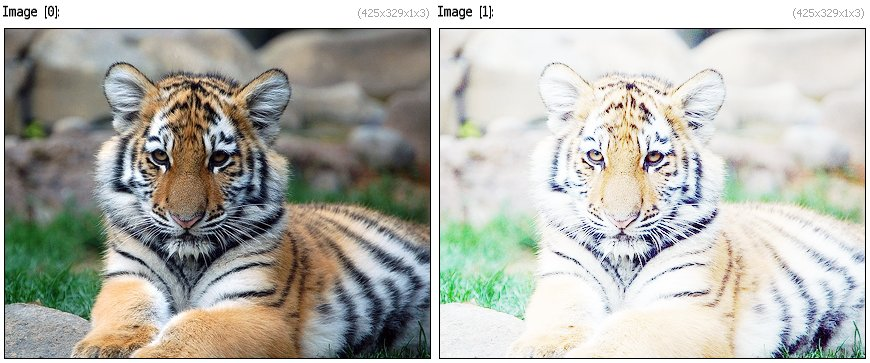
\includegraphics[keepaspectratio=true,height=7cm,width=\textwidth]{img/gmic_def46.jpg}\\
{\footnotesize \textbf{Example 46~:} \texttt{image.jpg -and \{128+64\}}}
\\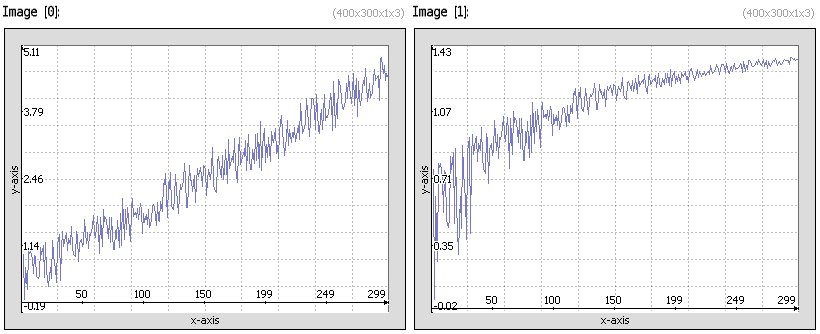
\includegraphics[keepaspectratio=true,height=7cm,width=\textwidth]{img/gmic_def47.jpg}\\
{\footnotesize \textbf{Example 47~:} \texttt{image.jpg --mirror x -and}}
\end{center}

\subsection{\emph{-asin\index{-asin}} (+)}\vspace*{-0.5em}
Compute the pointwise arc-sine of selected images.
\begin{center}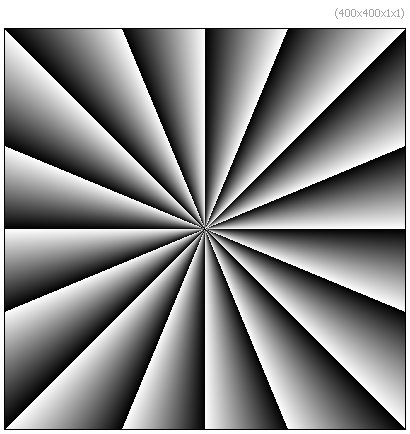
\includegraphics[keepaspectratio=true,height=7cm,width=\textwidth]{img/gmic_def48.jpg}\\
{\footnotesize \textbf{Example 48~:} \texttt{image.jpg --normalize -1,1 -asin[-1]}}
\\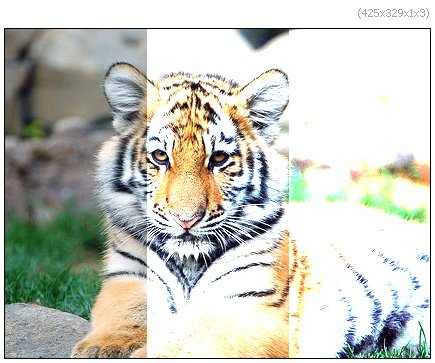
\includegraphics[keepaspectratio=true,height=7cm,width=\textwidth]{img/gmic_def49.jpg}\\
{\footnotesize \textbf{Example 49~:} \texttt{300,1,1,1,'x/w+0.1*u' --asin -display\_graph 400,300}}
\end{center}

\subsection{\emph{-atan\index{-atan}} (+)}\vspace*{-0.5em}
Compute the pointwise arc-tangent of selected images.
\begin{center}\includegraphics[keepaspectratio=true,height=7cm,width=\textwidth]{img/gmic_def50.jpg}\\
{\footnotesize \textbf{Example 50~:} \texttt{image.jpg --normalize 0,8 -atan[-1]}}
\\\includegraphics[keepaspectratio=true,height=7cm,width=\textwidth]{img/gmic_def51.jpg}\\
{\footnotesize \textbf{Example 51~:} \texttt{300,1,1,1,'4*x/w+u' --atan -display\_graph 400,300}}
\end{center}

\subsection{\emph{-atan2\index{-atan2}} (+)}\vspace*{-0.5em}
~\\\textbf{Arguments: } 
{\small \texttt{[x\_argument]}}\\~\\
Compute the pointwise oriented arc-tangent of selected images.
~\\Each selected image is regarded as the y-argument of the arc-tangent function, while the
specified image gives the corresponding x-argument.
\begin{center}\includegraphics[keepaspectratio=true,height=7cm,width=\textwidth]{img/gmic_def52.jpg}\\
{\footnotesize \textbf{Example 52~:} \texttt{(-1,1) (-1;1) -resize 400,400,1,1,3 -atan2[1] [0] -keep[1] -mod \{pi/8\}}}
\end{center}

\subsection{\emph{-bsl\index{-bsl}} (+)}\vspace*{-0.5em}
~\\\textbf{Arguments: } 
{\small \texttt{value[\%]}}~~~$|$\\
\hspace*{2.2cm}{\small \texttt{[image]}}~~~$|$\\
\hspace*{2.2cm}{\small \texttt{'formula'}}~~~$|$\\
\hspace*{2.2cm}{\small \texttt{(no args)}}\\~\\
Compute the bitwise left shift of selected images with specified value, image or
mathematical expression, or compute the pointwise sequential bitwise left shift of
selected images.
~\\(\emph{eq. to} {\small \texttt{'-$<$$<$'}}).
\begin{center}\includegraphics[keepaspectratio=true,height=7cm,width=\textwidth]{img/gmic_def53.jpg}\\
{\footnotesize \textbf{Example 53~:} \texttt{image.jpg -bsl 'round(3*x/w,0)' -cut 0,255}}
\end{center}

\subsection{\emph{-bsr\index{-bsr}} (+)}\vspace*{-0.5em}
~\\\textbf{Arguments: } 
{\small \texttt{value[\%]}}~~~$|$\\
\hspace*{2.2cm}{\small \texttt{[image]}}~~~$|$\\
\hspace*{2.2cm}{\small \texttt{'formula'}}~~~$|$\\
\hspace*{2.2cm}{\small \texttt{(no args)}}\\~\\
Compute the bitwise right shift of selected images with specified value, image or"
mathematical expression, or compute the pointwise sequential bitwise right shift of
selected images.
~\\(\emph{eq. to} {\small \texttt{'-$>$$>$'}}).
\begin{center}\includegraphics[keepaspectratio=true,height=7cm,width=\textwidth]{img/gmic_def54.jpg}\\
{\footnotesize \textbf{Example 54~:} \texttt{image.jpg -bsr 'round(3*x/w,0)' -cut 0,255}}
\end{center}

\subsection{\emph{-cos\index{-cos}} (+)}\vspace*{-0.5em}
Compute the pointwise cosine of selected images.
\begin{center}\includegraphics[keepaspectratio=true,height=7cm,width=\textwidth]{img/gmic_def55.jpg}\\
{\footnotesize \textbf{Example 55~:} \texttt{image.jpg --normalize 0,\{2*pi\} -cos[-1]}}
\\\includegraphics[keepaspectratio=true,height=7cm,width=\textwidth]{img/gmic_def56.jpg}\\
{\footnotesize \textbf{Example 56~:} \texttt{300,1,1,1,'20*x/w+u' --cos -display\_graph 400,300}}
\end{center}

\subsection{\emph{-cosh\index{-cosh}} (+)}\vspace*{-0.5em}
Compute the pointwise hyperbolic cosine of selected images.
\begin{center}\includegraphics[keepaspectratio=true,height=7cm,width=\textwidth]{img/gmic_def57.jpg}\\
{\footnotesize \textbf{Example 57~:} \texttt{image.jpg --normalize -3,3 -cosh[-1]}}
\\\includegraphics[keepaspectratio=true,height=7cm,width=\textwidth]{img/gmic_def58.jpg}\\
{\footnotesize \textbf{Example 58~:} \texttt{300,1,1,1,'4*x/w+u' --cosh -display\_graph 400,300}}
\end{center}

\subsection{\emph{-div\index{-div}} (+)}\vspace*{-0.5em}
~\\\textbf{Arguments: } 
{\small \texttt{value[\%]}}~~~$|$\\
\hspace*{2.2cm}{\small \texttt{[image]}}~~~$|$\\
\hspace*{2.2cm}{\small \texttt{'formula'}}~~~$|$\\
\hspace*{2.2cm}{\small \texttt{(no args)}}\\~\\
Divide selected image by specified value, image or mathematical expression,
or compute the pointwise quotient of selected images.
~\\(\emph{eq. to} {\small \texttt{'-/'}}).
\begin{center}\includegraphics[keepaspectratio=true,height=7cm,width=\textwidth]{img/gmic_def59.jpg}\\
{\footnotesize \textbf{Example 59~:} \texttt{image.jpg -div '1+abs(cos(x/10)*sin(y/10))'}}
\\\includegraphics[keepaspectratio=true,height=7cm,width=\textwidth]{img/gmic_def60.jpg}\\
{\footnotesize \textbf{Example 60~:} \texttt{image.jpg --luminance --div}}
\end{center}

\subsection{\emph{-eq\index{-eq}} (+)}\vspace*{-0.5em}
~\\\textbf{Arguments: } 
{\small \texttt{value[\%]}}~~~$|$\\
\hspace*{2.2cm}{\small \texttt{[image]}}~~~$|$\\
\hspace*{2.2cm}{\small \texttt{'formula'}}~~~$|$\\
\hspace*{2.2cm}{\small \texttt{(no args)}}\\~\\
Compute the boolean equality of selected images with specified value, image or
mathematical expression, or compute the boolean equality of selected images.
~\\(\emph{eq. to} {\small \texttt{'-=='}}).
\begin{center}\includegraphics[keepaspectratio=true,height=7cm,width=\textwidth]{img/gmic_def61.jpg}\\
{\footnotesize \textbf{Example 61~:} \texttt{image.jpg -round 40 -eq \{round(ia,40)\}}}
\\\includegraphics[keepaspectratio=true,height=7cm,width=\textwidth]{img/gmic_def62.jpg}\\
{\footnotesize \textbf{Example 62~:} \texttt{image.jpg --mirror x -eq}}
\end{center}

\subsection{\emph{-exp\index{-exp}} (+)}\vspace*{-0.5em}
Compute the pointwise exponential of selected images.
\begin{center}\includegraphics[keepaspectratio=true,height=7cm,width=\textwidth]{img/gmic_def63.jpg}\\
{\footnotesize \textbf{Example 63~:} \texttt{image.jpg --normalize 0,2 -exp[-1]}}
\\\includegraphics[keepaspectratio=true,height=7cm,width=\textwidth]{img/gmic_def64.jpg}\\
{\footnotesize \textbf{Example 64~:} \texttt{300,1,1,1,'7*x/w+u' --exp -display\_graph 400,300}}
\end{center}

\subsection{\emph{-ge\index{-ge}} (+)}\vspace*{-0.5em}
~\\\textbf{Arguments: } 
{\small \texttt{value[\%]}}~~~$|$\\
\hspace*{2.2cm}{\small \texttt{[image]}}~~~$|$\\
\hspace*{2.2cm}{\small \texttt{'formula'}}~~~$|$\\
\hspace*{2.2cm}{\small \texttt{(no args)}}\\~\\
Compute the boolean 'greater or equal than' of selected images with specified value, image
or mathematical expression, or compute the boolean 'greater or equal than' of selected images.
~\\(\emph{eq. to} {\small \texttt{'-$>$='}}).
\begin{center}\includegraphics[keepaspectratio=true,height=7cm,width=\textwidth]{img/gmic_def65.jpg}\\
{\footnotesize \textbf{Example 65~:} \texttt{image.jpg -ge \{ia\}}}
\\\includegraphics[keepaspectratio=true,height=7cm,width=\textwidth]{img/gmic_def66.jpg}\\
{\footnotesize \textbf{Example 66~:} \texttt{image.jpg --mirror x -ge}}
\end{center}

\subsection{\emph{-gt\index{-gt}} (+)}\vspace*{-0.5em}
~\\\textbf{Arguments: } 
{\small \texttt{value[\%]}}~~~$|$\\
\hspace*{2.2cm}{\small \texttt{[image]}}~~~$|$\\
\hspace*{2.2cm}{\small \texttt{'formula'}}~~~$|$\\
\hspace*{2.2cm}{\small \texttt{(no args)}}\\~\\
Compute the boolean 'greater than' of selected images with specified value, image or
mathematical expression, or compute the boolean 'greater than' of selected images.
~\\(\emph{eq. to} {\small \texttt{'-$>$'}}).
\begin{center}\includegraphics[keepaspectratio=true,height=7cm,width=\textwidth]{img/gmic_def67.jpg}\\
{\footnotesize \textbf{Example 67~:} \texttt{image.jpg -gt \{ia\}}}
\\\includegraphics[keepaspectratio=true,height=7cm,width=\textwidth]{img/gmic_def68.jpg}\\
{\footnotesize \textbf{Example 68~:} \texttt{image.jpg --mirror x -gt}}
\end{center}

\subsection{\emph{-le\index{-le}} (+)}\vspace*{-0.5em}
~\\\textbf{Arguments: } 
{\small \texttt{value[\%]}}~~~$|$\\
\hspace*{2.2cm}{\small \texttt{[image]}}~~~$|$\\
\hspace*{2.2cm}{\small \texttt{'formula'}}~~~$|$\\
\hspace*{2.2cm}{\small \texttt{(no args)}}\\~\\
Compute the boolean 'less or equal than' of selected images with specified value, image or
mathematical expression, or compute the boolean 'less or equal than' of selected images.
~\\(\emph{eq. to} {\small \texttt{'-$<$='}}).
\begin{center}\includegraphics[keepaspectratio=true,height=7cm,width=\textwidth]{img/gmic_def69.jpg}\\
{\footnotesize \textbf{Example 69~:} \texttt{image.jpg -le \{ia\}}}
\\\includegraphics[keepaspectratio=true,height=7cm,width=\textwidth]{img/gmic_def70.jpg}\\
{\footnotesize \textbf{Example 70~:} \texttt{image.jpg --mirror x -le}}
\end{center}

\subsection{\emph{-lt\index{-lt}} (+)}\vspace*{-0.5em}
~\\\textbf{Arguments: } 
{\small \texttt{value[\%]}}~~~$|$\\
\hspace*{2.2cm}{\small \texttt{[image]}}~~~$|$\\
\hspace*{2.2cm}{\small \texttt{'formula'}}~~~$|$\\
\hspace*{2.2cm}{\small \texttt{(no args)}}\\~\\
Compute the boolean 'less than' of selected images with specified value, image or
mathematical expression, or compute the boolean 'less than' of selected images.
~\\(\emph{eq. to} {\small \texttt{'-$<$'}}).
\begin{center}\includegraphics[keepaspectratio=true,height=7cm,width=\textwidth]{img/gmic_def71.jpg}\\
{\footnotesize \textbf{Example 71~:} \texttt{image.jpg -lt \{ia\}}}
\\\includegraphics[keepaspectratio=true,height=7cm,width=\textwidth]{img/gmic_def72.jpg}\\
{\footnotesize \textbf{Example 72~:} \texttt{image.jpg --mirror x -lt}}
\end{center}

\subsection{\emph{-log\index{-log}} (+)}\vspace*{-0.5em}
Compute the pointwise base-e logarithm of selected images.
\begin{center}\includegraphics[keepaspectratio=true,height=7cm,width=\textwidth]{img/gmic_def73.jpg}\\
{\footnotesize \textbf{Example 73~:} \texttt{image.jpg --add 1 -log[-1]}}
\\\includegraphics[keepaspectratio=true,height=7cm,width=\textwidth]{img/gmic_def74.jpg}\\
{\footnotesize \textbf{Example 74~:} \texttt{300,1,1,1,'7*x/w+u' --log -display\_graph 400,300}}
\end{center}

\subsection{\emph{-log10\index{-log10}} (+)}\vspace*{-0.5em}
Compute the pointwise base-10 logarithm of selected images.
\begin{center}\includegraphics[keepaspectratio=true,height=7cm,width=\textwidth]{img/gmic_def75.jpg}\\
{\footnotesize \textbf{Example 75~:} \texttt{image.jpg --add 1 -log10[-1]}}
\\\includegraphics[keepaspectratio=true,height=7cm,width=\textwidth]{img/gmic_def76.jpg}\\
{\footnotesize \textbf{Example 76~:} \texttt{300,1,1,1,'7*x/w+u' --log10 -display\_graph 400,300}}
\end{center}

\subsection{\emph{-log2\index{-log2}} (+)}\vspace*{-0.5em}
Compute the pointwise base-2 logarithm of selected images
\begin{center}\includegraphics[keepaspectratio=true,height=7cm,width=\textwidth]{img/gmic_def77.jpg}\\
{\footnotesize \textbf{Example 77~:} \texttt{image.jpg --add 1 -log2[-1]}}
\\\includegraphics[keepaspectratio=true,height=7cm,width=\textwidth]{img/gmic_def78.jpg}\\
{\footnotesize \textbf{Example 78~:} \texttt{300,1,1,1,'7*x/w+u' --log2 -display\_graph 400,300}}
\end{center}

\subsection{\emph{-max\index{-max}} (+)}\vspace*{-0.5em}
~\\\textbf{Arguments: } 
{\small \texttt{value[\%]}}~~~$|$\\
\hspace*{2.2cm}{\small \texttt{[image]}}~~~$|$\\
\hspace*{2.2cm}{\small \texttt{'formula'}}~~~$|$\\
\hspace*{2.2cm}{\small \texttt{(no args)}}\\~\\
Compute the maximum between selected images and specified value, image or
mathematical expression, or compute the pointwise maxima between selected images.
\begin{center}\includegraphics[keepaspectratio=true,height=7cm,width=\textwidth]{img/gmic_def79.jpg}\\
{\footnotesize \textbf{Example 79~:} \texttt{image.jpg --mirror x -max}}
\\\includegraphics[keepaspectratio=true,height=7cm,width=\textwidth]{img/gmic_def80.jpg}\\
{\footnotesize \textbf{Example 80~:} \texttt{image.jpg -max 'R=((x/w-0.5)\textasciicircum 2+(y/h-0.5)\textasciicircum 2)\textasciicircum 0.5;255*R'}}
\end{center}

\subsection{\emph{-mdiv\index{-mdiv}} (+)}\vspace*{-0.5em}
~\\\textbf{Arguments: } 
{\small \texttt{value[\%]}}~~~$|$\\
\hspace*{2.2cm}{\small \texttt{[image]}}~~~$|$\\
\hspace*{2.2cm}{\small \texttt{'formula'}}~~~$|$\\
\hspace*{2.2cm}{\small \texttt{(no args)}}\\~\\
Compute the matrix division of selected matrices/vectors by specified value, image or
mathematical expression, or compute the matrix division of selected images.
~\\(\emph{eq. to} {\small \texttt{'-//'}}).


\subsection{\emph{-min\index{-min}} (+)}\vspace*{-0.5em}
~\\\textbf{Arguments: } 
{\small \texttt{value[\%]}}~~~$|$\\
\hspace*{2.2cm}{\small \texttt{[image]}}~~~$|$\\
\hspace*{2.2cm}{\small \texttt{'formula'}}~~~$|$\\
\hspace*{2.2cm}{\small \texttt{(no args)}}\\~\\
Compute the minimum between selected images and specified value, image or
mathematical expression, or compute the pointwise minima between selected images.
\begin{center}\includegraphics[keepaspectratio=true,height=7cm,width=\textwidth]{img/gmic_def81.jpg}\\
{\footnotesize \textbf{Example 81~:} \texttt{image.jpg --mirror x -min}}
\\\includegraphics[keepaspectratio=true,height=7cm,width=\textwidth]{img/gmic_def82.jpg}\\
{\footnotesize \textbf{Example 82~:} \texttt{image.jpg -min 'R=((x/w-0.5)\textasciicircum 2+(y/h-0.5)\textasciicircum 2)\textasciicircum 0.5;255*R'}}
\end{center}

\subsection{\emph{-mod\index{-mod}} (+)}\vspace*{-0.5em}
~\\\textbf{Arguments: } 
{\small \texttt{value[\%]}}~~~$|$\\
\hspace*{2.2cm}{\small \texttt{[image]}}~~~$|$\\
\hspace*{2.2cm}{\small \texttt{'formula'}}~~~$|$\\
\hspace*{2.2cm}{\small \texttt{(no args)}}\\~\\
Compute the modulo of selected images with specified value, image or mathematical
expression, or compute the pointwise sequential modulo of selected images.
~\\(\emph{eq. to} {\small \texttt{'-\%'}}).
\begin{center}\includegraphics[keepaspectratio=true,height=7cm,width=\textwidth]{img/gmic_def83.jpg}\\
{\footnotesize \textbf{Example 83~:} \texttt{image.jpg --mirror x -mod}}
\\\includegraphics[keepaspectratio=true,height=7cm,width=\textwidth]{img/gmic_def84.jpg}\\
{\footnotesize \textbf{Example 84~:} \texttt{image.jpg -mod 'R=((x/w-0.5)\textasciicircum 2+(y/h-0.5)\textasciicircum 2)\textasciicircum 0.5;255*R'}}
\end{center}

\subsection{\emph{-mmul\index{-mmul}} (+)}\vspace*{-0.5em}
~\\\textbf{Arguments: } 
{\small \texttt{value[\%]}}~~~$|$\\
\hspace*{2.2cm}{\small \texttt{[image]}}~~~$|$\\
\hspace*{2.2cm}{\small \texttt{'formula'}}~~~$|$\\
\hspace*{2.2cm}{\small \texttt{(no args)}}\\~\\
Compute the matrix right multiplication of selected matrices/vectors by specified value, image or
mathematical expression, or compute the matrix right multiplication of selected images.
~\\(\emph{eq. to} {\small \texttt{'-**'}}).
\begin{center}\includegraphics[keepaspectratio=true,height=7cm,width=\textwidth]{img/gmic_def85.jpg}\\
{\footnotesize \textbf{Example 85~:} \texttt{(0,1,0;0,0,1;1,0,0) (1;2;3) --mmul}}
\end{center}

\subsection{\emph{-mul\index{-mul}} (+)}\vspace*{-0.5em}
~\\\textbf{Arguments: } 
{\small \texttt{value[\%]}}~~~$|$\\
\hspace*{2.2cm}{\small \texttt{[image]}}~~~$|$\\
\hspace*{2.2cm}{\small \texttt{'formula'}}~~~$|$\\
\hspace*{2.2cm}{\small \texttt{(no args)}}\\~\\
Multiply selected images by specified value, image or mathematical expression,
or compute the pointwise product of selected images.
~\\(\emph{eq. to} {\small \texttt{'-*'}}).
\begin{center}\includegraphics[keepaspectratio=true,height=7cm,width=\textwidth]{img/gmic_def86.jpg}\\
{\footnotesize \textbf{Example 86~:} \texttt{image.jpg --mul 2 -cut 0,255}}
\\\includegraphics[keepaspectratio=true,height=7cm,width=\textwidth]{img/gmic_def87.jpg}\\
{\footnotesize \textbf{Example 87~:} \texttt{image.jpg (1,2,3,4,5,6,7,8) -resize[-1] [0] -mul[0] [-1]}}
\\\includegraphics[keepaspectratio=true,height=7cm,width=\textwidth]{img/gmic_def88.jpg}\\
{\footnotesize \textbf{Example 88~:} \texttt{image.jpg -mul '1-3*abs(x/w-0.5)' -cut 0,255}}
\\\includegraphics[keepaspectratio=true,height=7cm,width=\textwidth]{img/gmic_def89.jpg}\\
{\footnotesize \textbf{Example 89~:} \texttt{image.jpg --luminance -negative[-1] --mul}}
\end{center}

\subsection{\emph{-neq\index{-neq}} (+)}\vspace*{-0.5em}
~\\\textbf{Arguments: } 
{\small \texttt{value[\%]}}~~~$|$\\
\hspace*{2.2cm}{\small \texttt{[image]}}~~~$|$\\
\hspace*{2.2cm}{\small \texttt{'formula'}}~~~$|$\\
\hspace*{2.2cm}{\small \texttt{(no args)}}\\~\\
Compute the boolean inequality of selected images with specified value, image or
mathematical expression, or compute the boolean inequality of selected images.
~\\(\emph{eq. to} {\small \texttt{'-!='}}).
\begin{center}\includegraphics[keepaspectratio=true,height=7cm,width=\textwidth]{img/gmic_def90.jpg}\\
{\footnotesize \textbf{Example 90~:} \texttt{image.jpg -round 40 -neq \{round(ia,40)\}}}
\end{center}

\subsection{\emph{-or\index{-or}} (+)}\vspace*{-0.5em}
~\\\textbf{Arguments: } 
{\small \texttt{value[\%]}}~~~$|$\\
\hspace*{2.2cm}{\small \texttt{[image]}}~~~$|$\\
\hspace*{2.2cm}{\small \texttt{'formula'}}~~~$|$\\
\hspace*{2.2cm}{\small \texttt{(no args)}}\\~\\
Compute the bitwise OR of selected images with specified value, image or mathematical
expression, or compute the pointwise sequential bitwise OR of selected images.
\begin{center}\includegraphics[keepaspectratio=true,height=7cm,width=\textwidth]{img/gmic_def91.jpg}\\
{\footnotesize \textbf{Example 91~:} \texttt{image.jpg -or 128}}
\\\includegraphics[keepaspectratio=true,height=7cm,width=\textwidth]{img/gmic_def92.jpg}\\
{\footnotesize \textbf{Example 92~:} \texttt{image.jpg --mirror x -or}}
\end{center}

\subsection{\emph{-pow\index{-pow}} (+)}\vspace*{-0.5em}
~\\\textbf{Arguments: } 
{\small \texttt{value[\%]}}~~~$|$\\
\hspace*{2.2cm}{\small \texttt{[image]}}~~~$|$\\
\hspace*{2.2cm}{\small \texttt{'formula'}}~~~$|$\\
\hspace*{2.2cm}{\small \texttt{(no args)}}\\~\\
Raise selected image to the power of specified value, image or mathematical
expression, or compute the pointwise sequential powers of selected images.
~\\(\emph{eq. to} {\small \texttt{'-\textasciicircum '}}).
\begin{center}\includegraphics[keepaspectratio=true,height=7cm,width=\textwidth]{img/gmic_def93.jpg}\\
{\footnotesize \textbf{Example 93~:} \texttt{image.jpg -div 255 --pow 0.5 -mul 255}}
\\\includegraphics[keepaspectratio=true,height=7cm,width=\textwidth]{img/gmic_def94.jpg}\\
{\footnotesize \textbf{Example 94~:} \texttt{image.jpg -gradient -pow 2 -add -pow 0.2}}
\end{center}

\subsection{\emph{-rol\index{-rol}} (+)}\vspace*{-0.5em}
~\\\textbf{Arguments: } 
{\small \texttt{value[\%]}}~~~$|$\\
\hspace*{2.2cm}{\small \texttt{[image]}}~~~$|$\\
\hspace*{2.2cm}{\small \texttt{'formula'}}~~~$|$\\
\hspace*{2.2cm}{\small \texttt{(no args)}}\\~\\
Compute the bitwise left rotation of selected images with specified value, image or
mathematical expression, or compute the pointwise sequential bitwise left rotation of
selected images.
\begin{center}\includegraphics[keepaspectratio=true,height=7cm,width=\textwidth]{img/gmic_def95.jpg}\\
{\footnotesize \textbf{Example 95~:} \texttt{image.jpg -rol 'round(3*x/w,0)' -cut 0,255}}
\end{center}

\subsection{\emph{-ror\index{-ror}} (+)}\vspace*{-0.5em}
~\\\textbf{Arguments: } 
{\small \texttt{value[\%]}}~~~$|$\\
\hspace*{2.2cm}{\small \texttt{[image]}}~~~$|$\\
\hspace*{2.2cm}{\small \texttt{'formula'}}~~~$|$\\
\hspace*{2.2cm}{\small \texttt{(no args)}}\\~\\
Compute the bitwise right rotation of selected images with specified value, image or
mathematical expression, or compute the pointwise sequential bitwise right rotation of
selected images.
\begin{center}\includegraphics[keepaspectratio=true,height=7cm,width=\textwidth]{img/gmic_def96.jpg}\\
{\footnotesize \textbf{Example 96~:} \texttt{image.jpg -ror 'round(3*x/w,0)' -cut 0,255}}
\end{center}

\subsection{\emph{-sign\index{-sign}} (+)}\vspace*{-0.5em}
Compute the pointwise sign of selected images.
\begin{center}\includegraphics[keepaspectratio=true,height=7cm,width=\textwidth]{img/gmic_def97.jpg}\\
{\footnotesize \textbf{Example 97~:} \texttt{image.jpg --sub \{ia\} -sign[-1]}}
\\\includegraphics[keepaspectratio=true,height=7cm,width=\textwidth]{img/gmic_def98.jpg}\\
{\footnotesize \textbf{Example 98~:} \texttt{300,1,1,1,'cos(20*x/w+u)' --sign -display\_graph 400,300}}
\end{center}

\subsection{\emph{-sin\index{-sin}} (+)}\vspace*{-0.5em}
Compute the pointwise sine of selected images.
\begin{center}\includegraphics[keepaspectratio=true,height=7cm,width=\textwidth]{img/gmic_def99.jpg}\\
{\footnotesize \textbf{Example 99~:} \texttt{image.jpg --normalize 0,\{2*pi\} -sin[-1]}}
\\\includegraphics[keepaspectratio=true,height=7cm,width=\textwidth]{img/gmic_def100.jpg}\\
{\footnotesize \textbf{Example 100~:} \texttt{300,1,1,1,'20*x/w+u' --sin -display\_graph 400,300}}
\end{center}

\subsection{\emph{-sinc\index{-sinc}} (+)}\vspace*{-0.5em}
Compute the pointwise sinc function of selected images.
\begin{center}\includegraphics[keepaspectratio=true,height=7cm,width=\textwidth]{img/gmic_def101.jpg}\\
{\footnotesize \textbf{Example 101~:} \texttt{image.jpg --normalize \{-2*pi\},\{2*pi\} -sinc[-1]}}
\\\includegraphics[keepaspectratio=true,height=7cm,width=\textwidth]{img/gmic_def102.jpg}\\
{\footnotesize \textbf{Example 102~:} \texttt{300,1,1,1,'20*x/w+u' --sinc -display\_graph 400,300}}
\end{center}

\subsection{\emph{-sinh\index{-sinh}} (+)}\vspace*{-0.5em}
Compute the pointwise hyperbolic sine of selected images.
\begin{center}\includegraphics[keepaspectratio=true,height=7cm,width=\textwidth]{img/gmic_def103.jpg}\\
{\footnotesize \textbf{Example 103~:} \texttt{image.jpg --normalize -3,3 -sinh[-1]}}
\\\includegraphics[keepaspectratio=true,height=7cm,width=\textwidth]{img/gmic_def104.jpg}\\
{\footnotesize \textbf{Example 104~:} \texttt{300,1,1,1,'4*x/w+u' --sinh -display\_graph 400,300}}
\end{center}

\subsection{\emph{-sqr\index{-sqr}} (+)}\vspace*{-0.5em}
Compute the pointwise square function of selected images.
\begin{center}\includegraphics[keepaspectratio=true,height=7cm,width=\textwidth]{img/gmic_def105.jpg}\\
{\footnotesize \textbf{Example 105~:} \texttt{image.jpg --sqr}}
\\\includegraphics[keepaspectratio=true,height=7cm,width=\textwidth]{img/gmic_def106.jpg}\\
{\footnotesize \textbf{Example 106~:} \texttt{300,1,1,1,'40*x/w+u' --sqr -display\_graph 400,300}}
\end{center}

\subsection{\emph{-sqrt\index{-sqrt}} (+)}\vspace*{-0.5em}
Compute the pointwise square root of selected images.
\begin{center}\includegraphics[keepaspectratio=true,height=7cm,width=\textwidth]{img/gmic_def107.jpg}\\
{\footnotesize \textbf{Example 107~:} \texttt{image.jpg --sqrt}}
\\\includegraphics[keepaspectratio=true,height=7cm,width=\textwidth]{img/gmic_def108.jpg}\\
{\footnotesize \textbf{Example 108~:} \texttt{300,1,1,1,'40*x/w+u' --sqrt -display\_graph 400,300}}
\end{center}

\subsection{\emph{-sub\index{-sub}} (+)}\vspace*{-0.5em}
~\\\textbf{Arguments: } 
{\small \texttt{value[\%]}}~~~$|$\\
\hspace*{2.2cm}{\small \texttt{[image]}}~~~$|$\\
\hspace*{2.2cm}{\small \texttt{'formula'}}~~~$|$\\
\hspace*{2.2cm}{\small \texttt{(no args)}}\\~\\
Subtract specified value, image or mathematical expression to selected images,
or compute the pointwise difference of selected images.
~\\(\emph{eq. to} {\small \texttt{'--'}}).
\begin{center}\includegraphics[keepaspectratio=true,height=7cm,width=\textwidth]{img/gmic_def109.jpg}\\
{\footnotesize \textbf{Example 109~:} \texttt{image.jpg --sub 30\% -cut 0,255}}
\\\includegraphics[keepaspectratio=true,height=7cm,width=\textwidth]{img/gmic_def110.jpg}\\
{\footnotesize \textbf{Example 110~:} \texttt{image.jpg --mirror x -sub[-1] [0]}}
\\\includegraphics[keepaspectratio=true,height=7cm,width=\textwidth]{img/gmic_def111.jpg}\\
{\footnotesize \textbf{Example 111~:} \texttt{image.jpg -sub 'i(w/2+0.9*(x-w/2),y)'}}
\\\includegraphics[keepaspectratio=true,height=7cm,width=\textwidth]{img/gmic_def112.jpg}\\
{\footnotesize \textbf{Example 112~:} \texttt{image.jpg --mirror x -sub}}
\end{center}

\subsection{\emph{-tan\index{-tan}} (+)}\vspace*{-0.5em}
Compute the pointwise tangent of selected images.
\begin{center}\includegraphics[keepaspectratio=true,height=7cm,width=\textwidth]{img/gmic_def113.jpg}\\
{\footnotesize \textbf{Example 113~:} \texttt{image.jpg --normalize \{-0.47*pi\},\{0.47*pi\} -tan[-1]}}
\\\includegraphics[keepaspectratio=true,height=7cm,width=\textwidth]{img/gmic_def114.jpg}\\
{\footnotesize \textbf{Example 114~:} \texttt{300,1,1,1,'20*x/w+u' --tan -display\_graph 400,300}}
\end{center}

\subsection{\emph{-tanh\index{-tanh}} (+)}\vspace*{-0.5em}
Compute the pointwise hyperbolic tangent of selected images.
\begin{center}\includegraphics[keepaspectratio=true,height=7cm,width=\textwidth]{img/gmic_def115.jpg}\\
{\footnotesize \textbf{Example 115~:} \texttt{image.jpg --normalize -3,3 -tanh[-1]}}
\\\includegraphics[keepaspectratio=true,height=7cm,width=\textwidth]{img/gmic_def116.jpg}\\
{\footnotesize \textbf{Example 116~:} \texttt{300,1,1,1,'4*x/w+u' --tanh -display\_graph 400,300}}
\end{center}

\subsection{\emph{-xor\index{-xor}} (+)}\vspace*{-0.5em}
~\\\textbf{Arguments: } 
{\small \texttt{value[\%]}}~~~$|$\\
\hspace*{2.2cm}{\small \texttt{[image]}}~~~$|$\\
\hspace*{2.2cm}{\small \texttt{'formula'}}~~~$|$\\
\hspace*{2.2cm}{\small \texttt{(no args)}}\\~\\
Compute the bitwise XOR of selected images with specified value, image or mathematical
expression, or compute the pointwise sequential bitwise XOR of selected images.
\begin{center}\includegraphics[keepaspectratio=true,height=7cm,width=\textwidth]{img/gmic_def117.jpg}\\
{\footnotesize \textbf{Example 117~:} \texttt{image.jpg -xor 128}}
\\\includegraphics[keepaspectratio=true,height=7cm,width=\textwidth]{img/gmic_def118.jpg}\\
{\footnotesize \textbf{Example 118~:} \texttt{image.jpg --mirror x -xor}}
\end{center}
\section{Values manipulation}


\subsection{\emph{-apply\_curve\index{-apply\_curve}} }\vspace*{-0.5em}
~\\\textbf{Arguments: } 
{\small \texttt{0$<$=smoothness$<$=1,x0,y0,x1,y1,x2,y2,...,xN,yN}}\\~\\
Apply curve transformation to image values.
~\\~\\\textbf{Default values}: {\small \texttt{'smoothness=1', 'x0=0', 'y0=100'.}}
\begin{center}\includegraphics[keepaspectratio=true,height=7cm,width=\textwidth]{img/gmic_def119.jpg}\\
{\footnotesize \textbf{Example 119~:} \texttt{image.jpg --apply\_curve 1,0,0,128,255,255,0}}
\end{center}

\subsection{\emph{-apply\_gamma\index{-apply\_gamma}} }\vspace*{-0.5em}
~\\\textbf{Arguments: } 
{\small \texttt{gamma$>$=0}}\\~\\
Apply gamma correction to selected images.
\begin{center}\includegraphics[keepaspectratio=true,height=7cm,width=\textwidth]{img/gmic_def120.jpg}\\
{\footnotesize \textbf{Example 120~:} \texttt{image.jpg --apply\_gamma 2}}
\end{center}

\subsection{\emph{-balance\_gamma\index{-balance\_gamma}} }\vspace*{-0.5em}
~\\\textbf{Arguments: } 
{\small \texttt{\_ref\_color1,...}}\\~\\
Apply color balance transformation on selected image, with respect to specified reference color.
~\\~\\\textbf{Default values}: {\small \texttt{'ref\_color1=128'.}}
\begin{center}\includegraphics[keepaspectratio=true,height=7cm,width=\textwidth]{img/gmic_def121.jpg}\\
{\footnotesize \textbf{Example 121~:} \texttt{image.jpg --balance\_gamma 128,64,64}}
\end{center}

\subsection{\emph{-complex2polar\index{-complex2polar}} }\vspace*{-0.5em}
Compute complex to polar transforms of selected images.
\begin{center}\includegraphics[keepaspectratio=true,height=7cm,width=\textwidth]{img/gmic_def122.jpg}\\
{\footnotesize \textbf{Example 122~:} \texttt{image.jpg --fft -complex2polar[-2,-1] -log[-2] -shift[-2] 50\%,50\%,0,0,2 -remove[-1]}}
\end{center}

\subsection{\emph{-compress\_rle\index{-compress\_rle}} }\vspace*{-0.5em}
Compress selected images as 2xN data matrices, using RLE algorithm.
\begin{center}\includegraphics[keepaspectratio=true,height=7cm,width=\textwidth]{img/gmic_def123.jpg}\\
{\footnotesize \textbf{Example 123~:} \texttt{image.jpg -resize2dy 100 -quantize 4 -round --compress\_rle --uncompress\_rle[-1]}}
\end{center}

\subsection{\emph{-cumul\index{-cumul}} }\vspace*{-0.5em}
Compute the cumulative function of specified image data.
\begin{center}\includegraphics[keepaspectratio=true,height=7cm,width=\textwidth]{img/gmic_def124.jpg}\\
{\footnotesize \textbf{Example 124~:} \texttt{image.jpg --histogram --cumul[-1] -display\_graph[-2,-1] 400,300,3}}
\end{center}

\subsection{\emph{-cut\index{-cut}} (+)}\vspace*{-0.5em}
~\\\textbf{Arguments: } 
{\small \texttt{\{ value0[\%] ~$|$~ [image0] \},\{ value1[\%] ~$|$~ [image1] \}}}~~~$|$\\
\hspace*{2.2cm}{\small \texttt{[image]}}~~~$|$\\
\hspace*{2.2cm}{\small \texttt{(no args)}}\\~\\
Cut values of selected images in specified range.
~\\(\emph{eq. to} {\small \texttt{'-c'}}).
~\\(noargs) runs interactive mode (uses the instant window [0] if opened).
\begin{center}\includegraphics[keepaspectratio=true,height=7cm,width=\textwidth]{img/gmic_def125.jpg}\\
{\footnotesize \textbf{Example 125~:} \texttt{image.jpg --add 30\% -cut[-1] 0,255}}
\\\includegraphics[keepaspectratio=true,height=7cm,width=\textwidth]{img/gmic_def126.jpg}\\
{\footnotesize \textbf{Example 126~:} \texttt{image.jpg --cut 25\%,75\%}}
\end{center}

\subsection{\emph{-discard\index{-discard}} }\vspace*{-0.5em}
~\\\textbf{Arguments: } 
{\small \texttt{value,\_remove\_if\_not\_found = \{ 0 ~$|$~ 1 \}.}}\\~\\
Remove specified value in selected images and return results as single-column vector.
~\\~\\\textbf{Default value}: {\small \texttt{'remove\_if\_not\_found=0'.}}
\begin{center}\includegraphics[keepaspectratio=true,height=7cm,width=\textwidth]{img/gmic_def127.jpg}\\
{\footnotesize \textbf{Example 127~:} \texttt{(1;2;3;4;3;2;1) --discard 2}}
\end{center}

\subsection{\emph{-eigen2tensor\index{-eigen2tensor}} }\vspace*{-0.5em}
Recompose selected pairs of eigenvalues/eigenvectors as 2x2 or 3x3 tensor fields.


\subsection{\emph{-endian\index{-endian}} (*)}\vspace*{-0.5em}
Reverse data endianness of selected images.


\subsection{\emph{-equalize\index{-equalize}} }\vspace*{-0.5em}
~\\\textbf{Arguments: } 
{\small \texttt{\_nb\_levels$>$0[\%],\_value\_min[\%],\_value\_max[\%]}}\\~\\
Equalize histograms of selected images.
~\\If value range is specified, the equalization is done only for pixels in the specified
value range.
~\\~\\\textbf{Default values}: {\small \texttt{'nb\_levels=256', 'value\_min=0\%'} and \texttt{'value\_max=100\%'.}}
\begin{center}\includegraphics[keepaspectratio=true,height=7cm,width=\textwidth]{img/gmic_def128.jpg}\\
{\footnotesize \textbf{Example 128~:} \texttt{image.jpg --equalize}}
\\\includegraphics[keepaspectratio=true,height=7cm,width=\textwidth]{img/gmic_def129.jpg}\\
{\footnotesize \textbf{Example 129~:} \texttt{image.jpg --equalize 4,0,128}}
\end{center}

\subsection{\emph{-fill\index{-fill}} (+)}\vspace*{-0.5em}
~\\\textbf{Arguments: } 
{\small \texttt{value1,\_value2,..}}~~~$|$\\
\hspace*{2.2cm}{\small \texttt{[image]}}~~~$|$\\
\hspace*{2.2cm}{\small \texttt{'formula'}}\\~\\
Fill selected images with values read from the specified value list, existing image
or mathematical expression. Single quotes may be omitted in 'formula'.
~\\(\emph{eq. to} {\small \texttt{'-f'}}).
\begin{center}\includegraphics[keepaspectratio=true,height=7cm,width=\textwidth]{img/gmic_def130.jpg}\\
{\footnotesize \textbf{Example 130~:} \texttt{4,4 -fill 1,2,3,4,5,6,7}}
\\\includegraphics[keepaspectratio=true,height=7cm,width=\textwidth]{img/gmic_def131.jpg}\\
{\footnotesize \textbf{Example 131~:} \texttt{4,4 (1,2,3,4,5,6,7) -fill[-2] [-1]}}
\\\includegraphics[keepaspectratio=true,height=7cm,width=\textwidth]{img/gmic_def132.jpg}\\
{\footnotesize \textbf{Example 132~:} \texttt{400,400,1,3 -fill "X=x-w/2; Y=y-h/2; R=sqrt(X\textasciicircum 2+Y\textasciicircum 2); a=atan2(Y,X); if (R$<$=180,255*abs(cos(c+200*(x/w-0.5)*(y/h-0.5))),850*(a\%(0.1*(c+1))))"}}
\end{center}

\subsection{\emph{-float2int8\index{-float2int8}} }\vspace*{-0.5em}
Convert selected float-valued images to 8bits integer representations.


\subsection{\emph{-int82float\index{-int82float}} }\vspace*{-0.5em}
Convert selected 8bits integer representations to float-valued images.


\subsection{\emph{-index\index{-index}} (+)}\vspace*{-0.5em}
~\\\textbf{Arguments: } 
{\small \texttt{\{ [palette] ~$|$~ predefined\_palette \},0$<$=\_dithering$<$=1,\_map\_palette=\{ 0 ~$|$~ 1 \}}}\\~\\
Index selected vector-valued images by specified vector-valued palette.
~\\'predefined\_palette' can be \{ 0=default ~$|$~ 1=HSV ~$|$~ 2=lines ~$|$~ 3=hot ~$|$~ 4=cool ~$|$~ 5=jet ~$|$~ 6=flag ~$|$~ 7=cube \}.
~\\~\\\textbf{Default values}: {\small \texttt{'dithering=0'} and \texttt{'map\_palette=0'.}}
\begin{center}\includegraphics[keepaspectratio=true,height=7cm,width=\textwidth]{img/gmic_def133.jpg}\\
{\footnotesize \textbf{Example 133~:} \texttt{image.jpg --index 1,1,1}}
\\\includegraphics[keepaspectratio=true,height=7cm,width=\textwidth]{img/gmic_def134.jpg}\\
{\footnotesize \textbf{Example 134~:} \texttt{image.jpg (0;255;255\textasciicircum 0;128;255\textasciicircum 0;0;255) --index[-2] [-1],1,1}}
\end{center}

\subsection{\emph{-image\_integral\index{-image\_integral}} }\vspace*{-0.5em}
Compute the image integral (summed area table) of selected images.
\begin{center}\includegraphics[keepaspectratio=true,height=7cm,width=\textwidth]{img/gmic_def135.jpg}\\
{\footnotesize \textbf{Example 135~:} \texttt{image.jpg --image\_integral}}
\end{center}

\subsection{\emph{-map\index{-map}} (+)}\vspace*{-0.5em}
~\\\textbf{Arguments: } 
{\small \texttt{[palette]}}~~~$|$\\
\hspace*{2.2cm}{\small \texttt{predefined\_palette}}\\~\\
Map specified vector-valued palette to selected indexed scalar images.
~\\'predefined\_palette' can be \{ 0=default ~$|$~ 1=HSV ~$|$~ 2=lines ~$|$~ 3=hot ~$|$~ 4=cool ~$|$~ 5=jet ~$|$~ 6=flag ~$|$~ 7=cube \}.
\begin{center}\includegraphics[keepaspectratio=true,height=7cm,width=\textwidth]{img/gmic_def136.jpg}\\
{\footnotesize \textbf{Example 136~:} \texttt{image.jpg --luminance -map[-1] 3}}
\\\includegraphics[keepaspectratio=true,height=7cm,width=\textwidth]{img/gmic_def137.jpg}\\
{\footnotesize \textbf{Example 137~:} \texttt{image.jpg --rgb2ycbcr -split[-1] c (0,255,0) -resize[-1] 256,1,1,1,3 -map[-4] [-1] -remove[-1] -append[-3--1] c -ycbcr2rgb[-1]}}
\end{center}

\subsection{\emph{-map\_clut\index{-map\_clut}} }\vspace*{-0.5em}
Map RGB color LUT image (regarded as the last image) to all other selected images.
\begin{center}\includegraphics[keepaspectratio=true,height=7cm,width=\textwidth]{img/gmic_def138.jpg}\\
{\footnotesize \textbf{Example 138~:} \texttt{image.jpg -uniform\_distribution \{2\textasciicircum 5\},3 -mirror[-1] x --map\_clut}}
\end{center}

\subsection{\emph{-mix\_channels\index{-mix\_channels}} }\vspace*{-0.5em}
~\\\textbf{Arguments: } 
{\small \texttt{(a00,...,aMN)}}\\~\\
Apply specified matrix to channels of selected images.
\begin{center}\includegraphics[keepaspectratio=true,height=7cm,width=\textwidth]{img/gmic_def139.jpg}\\
{\footnotesize \textbf{Example 139~:} \texttt{image.jpg --mix\_channels (0,1,0;1,0,0;0,0,1)}}
\end{center}

\subsection{\emph{-negative\index{-negative}} }\vspace*{-0.5em}
Compute negative of selected images.
\begin{center}\includegraphics[keepaspectratio=true,height=7cm,width=\textwidth]{img/gmic_def140.jpg}\\
{\footnotesize \textbf{Example 140~:} \texttt{image.jpg --negative}}
\end{center}

\subsection{\emph{-noise\index{-noise}} (+)}\vspace*{-0.5em}
~\\\textbf{Arguments: } 
{\small \texttt{std\_variation$>$=0[\%],\_noise\_type}}\\~\\
Add random noise to selected images.
~\\'noise\_type' can be \{ 0=gaussian ~$|$~ 1=uniform ~$|$~ 2=salt\&pepper ~$|$~ 3=poisson ~$|$~ 4=rice \}.
~\\~\\\textbf{Default value}: {\small \texttt{'noise\_type=0'.}}
\begin{center}\includegraphics[keepaspectratio=true,height=7cm,width=\textwidth]{img/gmic_def141.jpg}\\
{\footnotesize \textbf{Example 141~:} \texttt{image.jpg --noise[0] 50,0 --noise[0] 50,1 --noise[0] 10,2 -cut 0,255}}
\\\includegraphics[keepaspectratio=true,height=7cm,width=\textwidth]{img/gmic_def142.jpg}\\
{\footnotesize \textbf{Example 142~:} \texttt{300,300,1,3 [0] -noise[0] 20,0 -noise[1] 20,1 --histogram 100 -display\_graph[-2,-1] 400,300,3}}
\end{center}

\subsection{\emph{-norm\index{-norm}} }\vspace*{-0.5em}
Compute the pointwise euclidean norm of vector-valued pixels in selected images.
\begin{center}\includegraphics[keepaspectratio=true,height=7cm,width=\textwidth]{img/gmic_def143.jpg}\\
{\footnotesize \textbf{Example 143~:} \texttt{image.jpg --norm}}
\end{center}

\subsection{\emph{-normalize\index{-normalize}} (+)}\vspace*{-0.5em}
~\\\textbf{Arguments: } 
{\small \texttt{\{ value0[\%] ~$|$~ [image0] \},\{ value1[\%] ~$|$~ [image1] \}}}~~~$|$\\
\hspace*{2.2cm}{\small \texttt{[image]}}\\~\\
Linearly normalize values of selected images in specified range.
~\\(\emph{eq. to} {\small \texttt{'-n'}}).
\begin{center}\includegraphics[keepaspectratio=true,height=7cm,width=\textwidth]{img/gmic_def144.jpg}\\
{\footnotesize \textbf{Example 144~:} \texttt{image.jpg -split x,2 -normalize[-1] 64,196 -append x}}
\end{center}

\subsection{\emph{-normalize\_sum\index{-normalize\_sum}} }\vspace*{-0.5em}
Normalize selected images with a unitary sum.
\begin{center}\includegraphics[keepaspectratio=true,height=7cm,width=\textwidth]{img/gmic_def145.jpg}\\
{\footnotesize \textbf{Example 145~:} \texttt{image.jpg --histogram[-1] -normalize\_sum[-1] -display\_graph[-1] 400,300}}
\end{center}

\subsection{\emph{-orientation\index{-orientation}} }\vspace*{-0.5em}
Compute the pointwise orientation of vector-valued pixels in selected images.
\begin{center}\includegraphics[keepaspectratio=true,height=7cm,width=\textwidth]{img/gmic_def146.jpg}\\
{\footnotesize \textbf{Example 146~:} \texttt{image.jpg --orientation --norm[-2] -negative[-1] -mul[-2] [-1] -reverse[-2,-1]}}
\end{center}

\subsection{\emph{-otsu\index{-otsu}} }\vspace*{-0.5em}
~\\\textbf{Arguments: } 
{\small \texttt{\_nb\_levels$>$0}}\\~\\
Hard-threshold image using Otsu's method.
~\\~\\\textbf{Default value}: {\small \texttt{'nb\_levels=256'.}}
\begin{center}\includegraphics[keepaspectratio=true,height=7cm,width=\textwidth]{img/gmic_def147.jpg}\\
{\footnotesize \textbf{Example 147~:} \texttt{image.jpg -luminance --otsu ,}}
\end{center}

\subsection{\emph{-polar2complex\index{-polar2complex}} }\vspace*{-0.5em}
Compute polar to complex transforms of selected images.


\subsection{\emph{-quantize\index{-quantize}} }\vspace*{-0.5em}
~\\\textbf{Arguments: } 
{\small \texttt{nb\_levels$>$=1,\_keep\_values=\{ 0 ~$|$~ 1 \},\_is\_uniform=\{ 0 ~$|$~ 1 \}}}\\~\\
Quantize selected images.
~\\~\\\textbf{Default value}: {\small \texttt{'keep\_values=1'} and \texttt{'is\_uniform=0'.}}
\begin{center}\includegraphics[keepaspectratio=true,height=7cm,width=\textwidth]{img/gmic_def148.jpg}\\
{\footnotesize \textbf{Example 148~:} \texttt{image.jpg -luminance --quantize 3}}
\\\includegraphics[keepaspectratio=true,height=7cm,width=\textwidth]{img/gmic_def149.jpg}\\
{\footnotesize \textbf{Example 149~:} \texttt{200,200,1,1,'cos(x/10)*sin(y/10)' --quantize[0] 6 --quantize[0] 4 --quantize[0] 3 --quantize[0] 2}}
\end{center}

\subsection{\emph{-rand\index{-rand}} (+)}\vspace*{-0.5em}
~\\\textbf{Arguments: } 
{\small \texttt{\{ value0[\%] ~$|$~ [image0] \},\{ value1[\%] ~$|$~ [image1] \}}}~~~$|$\\
\hspace*{2.2cm}{\small \texttt{[image]}}\\~\\
Fill selected images with random values uniformly distributed in the specified range.
\begin{center}\includegraphics[keepaspectratio=true,height=7cm,width=\textwidth]{img/gmic_def150.jpg}\\
{\footnotesize \textbf{Example 150~:} \texttt{400,400,1,3 -rand -10,10 --blur 10 -sign[-1]}}
\end{center}

\subsection{\emph{-replace\index{-replace}} }\vspace*{-0.5em}
~\\\textbf{Arguments: } 
{\small \texttt{value\_src,value\_dest}}\\~\\
Replace pixel values in selected images.
\begin{center}\includegraphics[keepaspectratio=true,height=7cm,width=\textwidth]{img/gmic_def151.jpg}\\
{\footnotesize \textbf{Example 151~:} \texttt{(1;2;3;4) --replace 2,3}}
\end{center}

\subsection{\emph{-replace\_inf\index{-replace\_inf}} }\vspace*{-0.5em}
~\\\textbf{Arguments: } 
{\small \texttt{\_expression}}\\~\\
Replace all infinite values in selected images by specified expression.
\begin{center}\includegraphics[keepaspectratio=true,height=7cm,width=\textwidth]{img/gmic_def152.jpg}\\
{\footnotesize \textbf{Example 152~:} \texttt{(0;1;2) -log --replace\_inf 2}}
\end{center}

\subsection{\emph{-replace\_nan\index{-replace\_nan}} }\vspace*{-0.5em}
~\\\textbf{Arguments: } 
{\small \texttt{\_expression}}\\~\\
Replace all NaN values in selected images by specified expression.
\begin{center}\includegraphics[keepaspectratio=true,height=7cm,width=\textwidth]{img/gmic_def153.jpg}\\
{\footnotesize \textbf{Example 153~:} \texttt{(-1;0;2) -sqrt --replace\_nan 2}}
\end{center}

\subsection{\emph{-replace\_seq\index{-replace\_seq}} }\vspace*{-0.5em}
~\\\textbf{Arguments: } 
{\small \texttt{"search\_seq","replace\_seq"}}\\~\\
Search and replace a sequence of values in selected images.
\begin{center}\includegraphics[keepaspectratio=true,height=7cm,width=\textwidth]{img/gmic_def154.jpg}\\
{\footnotesize \textbf{Example 154~:} \texttt{(1;2;3;4;5) --replace\_seq "2,3,4","7,8"}}
\end{center}

\subsection{\emph{-round\index{-round}} (+)}\vspace*{-0.5em}
~\\\textbf{Arguments: } 
{\small \texttt{rounding\_value$>$=0,\_rounding\_type}}~~~$|$\\
\hspace*{2.2cm}{\small \texttt{(no args)}}\\~\\
Round values of selected images.
~\\'rounding\_type' can be \{ -1=backward ~$|$~ 0=nearest ~$|$~ 1=forward \}.
~\\~\\\textbf{Default value}: {\small \texttt{'rounding\_type=0'.}}
\begin{center}\includegraphics[keepaspectratio=true,height=7cm,width=\textwidth]{img/gmic_def155.jpg}\\
{\footnotesize \textbf{Example 155~:} \texttt{image.jpg --round 100}}
\\\includegraphics[keepaspectratio=true,height=7cm,width=\textwidth]{img/gmic_def156.jpg}\\
{\footnotesize \textbf{Example 156~:} \texttt{image.jpg -mul \{pi/180\} -sin --round}}
\end{center}

\subsection{\emph{-roundify\index{-roundify}} }\vspace*{-0.5em}
~\\\textbf{Arguments: } 
{\small \texttt{gamma$>$=0}}\\~\\
Apply roundify transformation on float-valued data, with specified gamma.
~\\~\\\textbf{Default value}: {\small \texttt{'gamma=0'.}}
\begin{center}\includegraphics[keepaspectratio=true,height=7cm,width=\textwidth]{img/gmic_def157.jpg}\\
{\footnotesize \textbf{Example 157~:} \texttt{1000 -fill '4*x/w' -repeat 5 --roundify[0] \{\$$>$*0.2\} -done -append c -display\_graph 400,300}}
\end{center}

\subsection{\emph{-set\index{-set}} (*)}\vspace*{-0.5em}
~\\\textbf{Arguments: } 
{\small \texttt{value,\_x[\%],\_y[\%],\_z[\%],\_c[\%]}}\\~\\
Set pixel value in selected images, at specified coordinates.
~\\(\emph{eq. to} {\small \texttt{'-='}}).
~\\If specified coordinates are outside the image bounds, no action is performed.
~\\~\\\textbf{Default values}: {\small \texttt{'x=y=z=c=0'.}}
\begin{center}\includegraphics[keepaspectratio=true,height=7cm,width=\textwidth]{img/gmic_def158.jpg}\\
{\footnotesize \textbf{Example 158~:} \texttt{2,2 -set 1,0,0 -set 2,1,0 -set 3,0,1 -set 4,1,1}}
\\\includegraphics[keepaspectratio=true,height=7cm,width=\textwidth]{img/gmic_def159.jpg}\\
{\footnotesize \textbf{Example 159~:} \texttt{image.jpg -repeat 10000 -set 255,\{?(100)\}\%,\{?(100)\}\%,0,\{?(100)\}\% -done}}
\end{center}

\subsection{\emph{-threshold\index{-threshold}} (+)}\vspace*{-0.5em}
~\\\textbf{Arguments: } 
{\small \texttt{value[\%],\_is\_soft}}~~~$|$\\
\hspace*{2.2cm}{\small \texttt{(no args)}}\\~\\
Threshold values of selected images.
~\\'soft' can be \{ 0=hard-thresholding ~$|$~ 1=soft-thresholding \}.
~\\(noargs) runs interactive mode (uses the instant window [0] if opened).
~\\~\\\textbf{Default value}: {\small \texttt{'is\_soft=0'.}}
\begin{center}\includegraphics[keepaspectratio=true,height=7cm,width=\textwidth]{img/gmic_def160.jpg}\\
{\footnotesize \textbf{Example 160~:} \texttt{image.jpg --threshold[0] 50\% --threshold[0] 50\%,1}}
\end{center}

\subsection{\emph{-threshold2\index{-threshold2}} }\vspace*{-0.5em}
~\\\textbf{Arguments: } 
{\small \texttt{min[\%],max[\%]}}\\~\\
Threshold selected images between the two given values.
~\\(\emph{eq. to} {\small \texttt{'-t2'}}).
\begin{center}\includegraphics[keepaspectratio=true,height=7cm,width=\textwidth]{img/gmic_def161.jpg}\\
{\footnotesize \textbf{Example 161~:} \texttt{image.jpg --threshold2 25\%,75\%}}
\end{center}

\subsection{\emph{-uncompress\_rle\index{-uncompress\_rle}} }\vspace*{-0.5em}
Uncompress selected 2xN data matrices, using RLE algorithm.


\subsection{\emph{-unrepeat\index{-unrepeat}} }\vspace*{-0.5em}
Remove repetition of adjacent values in selected images.
\begin{center}\includegraphics[keepaspectratio=true,height=7cm,width=\textwidth]{img/gmic_def162.jpg}\\
{\footnotesize \textbf{Example 162~:} \texttt{(1;1;1;1;1;2;2;2;3;4;4;4;5;5;5) --unrepeat}}
\end{center}

\subsection{\emph{-vector2tensor\index{-vector2tensor}} }\vspace*{-0.5em}
Convert selected vector fields to corresponding diffusion tensor fields.

\section{Colors manipulation}


\subsection{\emph{-apply\_channels\index{-apply\_channels}} }\vspace*{-0.5em}
~\\\textbf{Arguments: } 
{\small \texttt{"command",\_channels=\{ all=0 ~$|$~ rgba=1 ~$|$~ rgb=2 ~$|$~ y=3 ~$|$~ cbcr=4 ~$|$~ cb=5 ~$|$~ cr=6 ~$|$~ l=7 ~$|$~ ab=8 ~$|$~ a=9 ~$|$~ b=10 ~$|$~ h=11 ~$|$~ s=12 ~$|$~ v=13 ~$|$~ k=14 ~$|$~ cg=15 ~$|$~ ch=16 ~$|$~ c=17 ~$|$~ H=18 ~$|$~ r=19 ~$|$~ g=20 ~$|$~ b=21 ~$|$~ alpha==22 \},\_normalize=\{ 0=cut ~$|$~ 1=normalize \}}}\\~\\
Apply specified command on chosen normalized channels of each selected images.
~\\~\\\textbf{Default value}: {\small \texttt{'normalize=0'.}}
\begin{center}\includegraphics[keepaspectratio=true,height=7cm,width=\textwidth]{img/gmic_def163.jpg}\\
{\footnotesize \textbf{Example 163~:} \texttt{image.jpg --apply\_channels "-equalize -blur 2",5}}
\end{center}

\subsection{\emph{-autoindex\index{-autoindex}} }\vspace*{-0.5em}
~\\\textbf{Arguments: } 
{\small \texttt{nb\_colors$>$0,0$<$=\_dithering$<$=1,\_method=\{ 0=median-cut ~$|$~ 1=k-means \}}}\\~\\
Index selected vector-valued images by adapted colormaps.
~\\~\\\textbf{Default values}: {\small \texttt{'dithering=0'} and \texttt{'method=0'.}}
\begin{center}\includegraphics[keepaspectratio=true,height=7cm,width=\textwidth]{img/gmic_def164.jpg}\\
{\footnotesize \textbf{Example 164~:} \texttt{image.jpg --autoindex[0] 4 --autoindex[0] 8 --autoindex[0] 16}}
\end{center}

\subsection{\emph{-bayer2rgb\index{-bayer2rgb}} }\vspace*{-0.5em}
~\\\textbf{Arguments: } 
{\small \texttt{\_GM\_smoothness,\_RB\_smoothness1,\_RB\_smoothness2}}\\~\\
Transform selected RGB-Bayer sampled images to color images.
~\\~\\\textbf{Default values}: {\small \texttt{'GM\_smoothness=RB\_smoothness=1'} and \texttt{'RB\_smoothness2=0.5'.}}
\begin{center}\includegraphics[keepaspectratio=true,height=7cm,width=\textwidth]{img/gmic_def165.jpg}\\
{\footnotesize \textbf{Example 165~:} \texttt{image.jpg -rgb2bayer 0 --bayer2rgb 1,1,0.5}}
\end{center}

\subsection{\emph{-cmy2rgb\index{-cmy2rgb}} }\vspace*{-0.5em}
Convert selected images from CMY to RGB colorbases.


\subsection{\emph{-cmyk2rgb\index{-cmyk2rgb}} }\vspace*{-0.5em}
Convert selected images from CMYK to RGB colorbases.


\subsection{\emph{-colormap\index{-colormap}} }\vspace*{-0.5em}
~\\\textbf{Arguments: } 
{\small \texttt{nb\_levels$>$=1,\_method=\{ 0=median-cut ~$|$~ 1=k-means \},\_sort\_vectors=\{ 0 ~$|$~ 1 \}}}\\~\\
Estimate best-fitting colormap with 'nb\_colors' entries, to index selected images.
~\\~\\\textbf{Default value}: {\small \texttt{'method=0'} and \texttt{'sort\_vectors=1'.}}
\begin{center}\includegraphics[keepaspectratio=true,height=7cm,width=\textwidth]{img/gmic_def166.jpg}\\
{\footnotesize \textbf{Example 166~:} \texttt{image.jpg --colormap[0] 4 --colormap[0] 8 --colormap[0] 16}}
\end{center}

\subsection{\emph{-compose\_channels\index{-compose\_channels}} }\vspace*{-0.5em}
Compose all channels of each selected image, using specified arithmetic operator (+,-,or,min,...).
~\\~\\\textbf{Default value}: {\small \texttt{'1=+'.}}
\begin{center}\includegraphics[keepaspectratio=true,height=7cm,width=\textwidth]{img/gmic_def167.jpg}\\
{\footnotesize \textbf{Example 167~:} \texttt{image.jpg --compose\_channels and}}
\end{center}

\subsection{\emph{-direction2rgb\index{-direction2rgb}} }\vspace*{-0.5em}
Compute RGB representation of selected 2d direction fields.
\begin{center}\includegraphics[keepaspectratio=true,height=7cm,width=\textwidth]{img/gmic_def168.jpg}\\
{\footnotesize \textbf{Example 168~:} \texttt{image.jpg -luminance -gradient -append c -blur 2 -orientation --direction2rgb}}
\end{center}

\subsection{\emph{-ditheredbw\index{-ditheredbw}} }\vspace*{-0.5em}
Create dithered B\&W version of selected images.
\begin{center}\includegraphics[keepaspectratio=true,height=7cm,width=\textwidth]{img/gmic_def169.jpg}\\
{\footnotesize \textbf{Example 169~:} \texttt{image.jpg --equalize -ditheredbw[-1]}}
\end{center}

\subsection{\emph{-fill\_color\index{-fill\_color}} }\vspace*{-0.5em}
~\\\textbf{Arguments: } 
{\small \texttt{col1,...,colN}}\\~\\
Fill selected images with specified color.
~\\(\emph{eq. to} {\small \texttt{'-fc'}}).
\begin{center}\includegraphics[keepaspectratio=true,height=7cm,width=\textwidth]{img/gmic_def170.jpg}\\
{\footnotesize \textbf{Example 170~:} \texttt{image.jpg --fill\_color 255,0,255}}
\end{center}

\subsection{\emph{-gradient2rgb\index{-gradient2rgb}} }\vspace*{-0.5em}
~\\\textbf{Arguments: } 
{\small \texttt{\_is\_orientation=\{ 0 ~$|$~ 1 \}}}\\~\\
Compute RGB representation of 2d gradient of selected images.
~\\~\\\textbf{Default value}: {\small \texttt{'is\_orientation=0'.}}
\begin{center}\includegraphics[keepaspectratio=true,height=7cm,width=\textwidth]{img/gmic_def171.jpg}\\
{\footnotesize \textbf{Example 171~:} \texttt{image.jpg --gradient2rgb 0 -equalize[-1]}}
\end{center}

\subsection{\emph{-hsi2rgb\index{-hsi2rgb}} (+)}\vspace*{-0.5em}
Convert selected images from HSI to RGB colorbases.


\subsection{\emph{-hsi82rgb\index{-hsi82rgb}} }\vspace*{-0.5em}
Convert selected images from HSI8 to RGB color bases.


\subsection{\emph{-hsl2rgb\index{-hsl2rgb}} (+)}\vspace*{-0.5em}
Convert selected images from HSL to RGB colorbases.


\subsection{\emph{-hsl82rgb\index{-hsl82rgb}} }\vspace*{-0.5em}
Convert selected images from HSL8 to RGB color bases.


\subsection{\emph{-hsv2rgb\index{-hsv2rgb}} (+)}\vspace*{-0.5em}
Convert selected images from HSV to RGB colorbases.
\begin{center}\includegraphics[keepaspectratio=true,height=7cm,width=\textwidth]{img/gmic_def172.jpg}\\
{\footnotesize \textbf{Example 172~:} \texttt{(0,360;0,360\textasciicircum 0,0;1,1\textasciicircum 1,1;1,1) -resize 400,400,1,3,3 -hsv2rgb}}
\end{center}

\subsection{\emph{-hsv82rgb\index{-hsv82rgb}} }\vspace*{-0.5em}
Convert selected images from HSV8 to RGB color bases.


\subsection{\emph{-lab2lch\index{-lab2lch}} }\vspace*{-0.5em}
Convert selected images from Lab to Lch color bases.


\subsection{\emph{-lab2rgb\index{-lab2rgb}} (+)}\vspace*{-0.5em}
Convert selected images from Lab to RGB colorbases.
\begin{center}\includegraphics[keepaspectratio=true,height=7cm,width=\textwidth]{img/gmic_def173.jpg}\\
{\footnotesize \textbf{Example 173~:} \texttt{(50,50;50,50\textasciicircum -3,3;-3,3\textasciicircum -3,-3;3,3) -resize 400,400,1,3,3 -lab2rgb}}
\end{center}

\subsection{\emph{-lab82rgb\index{-lab82rgb}} }\vspace*{-0.5em}
Convert selected images from Lab8 to RGB color bases.


\subsection{\emph{-lch2lab\index{-lch2lab}} }\vspace*{-0.5em}
Convert selected images from Lch to Lab color bases.


\subsection{\emph{-lch2rgb\index{-lch2rgb}} }\vspace*{-0.5em}
Convert selected images from Lch to RGB color bases.


\subsection{\emph{-lch82rgb\index{-lch82rgb}} }\vspace*{-0.5em}
Convert selected images from Lch8 to RGB color bases.


\subsection{\emph{-luminance\index{-luminance}} }\vspace*{-0.5em}
Compute luminance of selected sRGB images.
\begin{center}\includegraphics[keepaspectratio=true,height=7cm,width=\textwidth]{img/gmic_def174.jpg}\\
{\footnotesize \textbf{Example 174~:} \texttt{image.jpg --luminance}}
\end{center}

\subsection{\emph{-mix\_rgb\index{-mix\_rgb}} }\vspace*{-0.5em}
~\\\textbf{Arguments: } 
{\small \texttt{a11,a12,a13,a21,a22,a23,a31,a32,a33}}\\~\\
Apply 3x3 specified matrix to RGB colors of selected images.
~\\~\\\textbf{Default values}: {\small \texttt{'a11=1', 'a12=a13=a21=0', 'a22=1', 'a23=a31=a32=0'} and \texttt{'a33=1'.}}
\begin{center}\includegraphics[keepaspectratio=true,height=7cm,width=\textwidth]{img/gmic_def175.jpg}\\
{\footnotesize \textbf{Example 175~:} \texttt{image.jpg --mix\_rgb 0,1,0,1,0,0,0,0,1}}
\end{center}

\subsection{\emph{-pseudogray\index{-pseudogray}} }\vspace*{-0.5em}
~\\\textbf{Arguments: } 
{\small \texttt{\_max\_increment$>$=0,\_JND\_threshold$>$=0,\_bits\_depth$>$0}}\\~\\
Generate pseudogray colormap with specified increment and perceptual threshold.
~\\If 'JND\_threshold' is 0, no perceptual constraints are applied.
~\\~\\\textbf{Default values}: {\small \texttt{'max\_increment=5', 'JND\_threshold=2.3'} and \texttt{'bits\_depth=8'.}}
\begin{center}\includegraphics[keepaspectratio=true,height=7cm,width=\textwidth]{img/gmic_def176.jpg}\\
{\footnotesize \textbf{Example 176~:} \texttt{-pseudogray 5}}
\end{center}

\subsection{\emph{-replace\_color\index{-replace\_color}} }\vspace*{-0.5em}
~\\\textbf{Arguments: } 
{\small \texttt{tolerance[\%]$>$=0,smoothness[\%]$>$=0,src1,src2,...,dest1,dest2,...}}\\~\\
Replace pixels from/to specified colors in selected images.
\begin{center}\includegraphics[keepaspectratio=true,height=7cm,width=\textwidth]{img/gmic_def177.jpg}\\
{\footnotesize \textbf{Example 177~:} \texttt{image.jpg --replace\_color 40,3,204,153,110,255,0,0}}
\end{center}

\subsection{\emph{-rgb2bayer\index{-rgb2bayer}} }\vspace*{-0.5em}
~\\\textbf{Arguments: } 
{\small \texttt{\_start\_pattern=0,\_color\_grid=0}}\\~\\
Transform selected color images to RGB-Bayer sampled images.
~\\~\\\textbf{Default values}: {\small \texttt{'start\_pattern=0'} and \texttt{'color\_grid=0'.}}
\begin{center}\includegraphics[keepaspectratio=true,height=7cm,width=\textwidth]{img/gmic_def178.jpg}\\
{\footnotesize \textbf{Example 178~:} \texttt{image.jpg --rgb2bayer 0}}
\end{center}

\subsection{\emph{-rgb2cmy\index{-rgb2cmy}} }\vspace*{-0.5em}
Convert selected images from RGB to CMY colorbases.
\begin{center}\includegraphics[keepaspectratio=true,height=7cm,width=\textwidth]{img/gmic_def179.jpg}\\
{\footnotesize \textbf{Example 179~:} \texttt{image.jpg -rgb2cmy -split c}}
\end{center}

\subsection{\emph{-rgb2cmyk\index{-rgb2cmyk}} }\vspace*{-0.5em}
Convert selected images from RGB to CMYK colorbases.
\begin{center}\includegraphics[keepaspectratio=true,height=7cm,width=\textwidth]{img/gmic_def180.jpg}\\
{\footnotesize \textbf{Example 180~:} \texttt{image.jpg -rgb2cmyk -split c}}
\\\includegraphics[keepaspectratio=true,height=7cm,width=\textwidth]{img/gmic_def181.jpg}\\
{\footnotesize \textbf{Example 181~:} \texttt{image.jpg -rgb2cmyk -split c -fill[3] 0 -append c -cmyk2rgb}}
\end{center}

\subsection{\emph{-rgb2hsi\index{-rgb2hsi}} (+)}\vspace*{-0.5em}
Convert selected images from RGB to HSI colorbases.
\begin{center}\includegraphics[keepaspectratio=true,height=7cm,width=\textwidth]{img/gmic_def182.jpg}\\
{\footnotesize \textbf{Example 182~:} \texttt{image.jpg -rgb2hsi -split c}}
\end{center}

\subsection{\emph{-rgb2hsi8\index{-rgb2hsi8}} }\vspace*{-0.5em}
Convert selected images from RGB to HSI8 color bases.
\begin{center}\includegraphics[keepaspectratio=true,height=7cm,width=\textwidth]{img/gmic_def183.jpg}\\
{\footnotesize \textbf{Example 183~:} \texttt{image.jpg -rgb2hsi8 -split c}}
\end{center}

\subsection{\emph{-rgb2hsl\index{-rgb2hsl}} (+)}\vspace*{-0.5em}
Convert selected images from RGB to HSL colorbases.
\begin{center}\includegraphics[keepaspectratio=true,height=7cm,width=\textwidth]{img/gmic_def184.jpg}\\
{\footnotesize \textbf{Example 184~:} \texttt{image.jpg -rgb2hsl -split c}}
\\\includegraphics[keepaspectratio=true,height=7cm,width=\textwidth]{img/gmic_def185.jpg}\\
{\footnotesize \textbf{Example 185~:} \texttt{image.jpg -rgb2hsl --split c -add[-3] 100 -mod[-3] 360 -append[-3--1] c -hsl2rgb}}
\end{center}

\subsection{\emph{-rgb2hsl8\index{-rgb2hsl8}} }\vspace*{-0.5em}
Convert selected images from RGB to HSL8 color bases.
\begin{center}\includegraphics[keepaspectratio=true,height=7cm,width=\textwidth]{img/gmic_def186.jpg}\\
{\footnotesize \textbf{Example 186~:} \texttt{image.jpg -rgb2hsl8 -split c}}
\end{center}

\subsection{\emph{-rgb2hsv\index{-rgb2hsv}} (+)}\vspace*{-0.5em}
Convert selected images from RGB to HSV colorbases.
\begin{center}\includegraphics[keepaspectratio=true,height=7cm,width=\textwidth]{img/gmic_def187.jpg}\\
{\footnotesize \textbf{Example 187~:} \texttt{image.jpg -rgb2hsv -split c}}
\\\includegraphics[keepaspectratio=true,height=7cm,width=\textwidth]{img/gmic_def188.jpg}\\
{\footnotesize \textbf{Example 188~:} \texttt{image.jpg -rgb2hsv --split c -add[-2] 0.3 -cut[-2] 0,1 -append[-3--1] c -hsv2rgb}}
\end{center}

\subsection{\emph{-rgb2hsv8\index{-rgb2hsv8}} }\vspace*{-0.5em}
Convert selected images from RGB to HSV8 color bases.
\begin{center}\includegraphics[keepaspectratio=true,height=7cm,width=\textwidth]{img/gmic_def189.jpg}\\
{\footnotesize \textbf{Example 189~:} \texttt{image.jpg -rgb2hsv8 -split c}}
\end{center}

\subsection{\emph{-rgb2lab\index{-rgb2lab}} (+)}\vspace*{-0.5em}
Convert selected images from RGB to Lab colorbases.
\begin{center}\includegraphics[keepaspectratio=true,height=7cm,width=\textwidth]{img/gmic_def190.jpg}\\
{\footnotesize \textbf{Example 190~:} \texttt{image.jpg -rgb2lab -split c}}
\\\includegraphics[keepaspectratio=true,height=7cm,width=\textwidth]{img/gmic_def191.jpg}\\
{\footnotesize \textbf{Example 191~:} \texttt{image.jpg -rgb2lab --split c -mul[-2,-1] 2.5 -append[-3--1] c -lab2rgb}}
\end{center}

\subsection{\emph{-rgb2lab8\index{-rgb2lab8}} }\vspace*{-0.5em}
Convert selected images from RGB to Lab8 color bases.
\begin{center}\includegraphics[keepaspectratio=true,height=7cm,width=\textwidth]{img/gmic_def192.jpg}\\
{\footnotesize \textbf{Example 192~:} \texttt{image.jpg -rgb2lab8 -split c}}
\end{center}

\subsection{\emph{-rgb2lch\index{-rgb2lch}} }\vspace*{-0.5em}
Convert selected images from RGB to Lch color bases.
\begin{center}\includegraphics[keepaspectratio=true,height=7cm,width=\textwidth]{img/gmic_def193.jpg}\\
{\footnotesize \textbf{Example 193~:} \texttt{image.jpg -rgb2lch -split c}}
\end{center}

\subsection{\emph{-rgb2lch8\index{-rgb2lch8}} }\vspace*{-0.5em}
Convert selected images from RGB to Lch8 color bases.
\begin{center}\includegraphics[keepaspectratio=true,height=7cm,width=\textwidth]{img/gmic_def194.jpg}\\
{\footnotesize \textbf{Example 194~:} \texttt{image.jpg -rgb2lch8 -split c}}
\end{center}

\subsection{\emph{-rgb2luv\index{-rgb2luv}} }\vspace*{-0.5em}
Convert selected images from RGB to LUV color bases.
\begin{center}\includegraphics[keepaspectratio=true,height=7cm,width=\textwidth]{img/gmic_def195.jpg}\\
{\footnotesize \textbf{Example 195~:} \texttt{image.jpg -rgb2luv -split c}}
\end{center}

\subsection{\emph{-rgb2srgb\index{-rgb2srgb}} (+)}\vspace*{-0.5em}
Convert selected images from RGB to sRGB colorbases.


\subsection{\emph{-rgb2xyz\index{-rgb2xyz}} }\vspace*{-0.5em}
Convert selected images from RGB to XYZ colorbases.
the D65 illuminant is used as the white point).
\begin{center}\includegraphics[keepaspectratio=true,height=7cm,width=\textwidth]{img/gmic_def196.jpg}\\
{\footnotesize \textbf{Example 196~:} \texttt{image.jpg -rgb2xyz -split c}}
\end{center}

\subsection{\emph{-rgb2xyz8\index{-rgb2xyz8}} }\vspace*{-0.5em}
Convert selected images from RGB to XYZ8 color bases.
\begin{center}\includegraphics[keepaspectratio=true,height=7cm,width=\textwidth]{img/gmic_def197.jpg}\\
{\footnotesize \textbf{Example 197~:} \texttt{image.jpg -rgb2xyz8 -split c}}
\end{center}

\subsection{\emph{-rgb2ycbcr\index{-rgb2ycbcr}} }\vspace*{-0.5em}
Convert selected images from RGB to YCbCr colorbases.
\begin{center}\includegraphics[keepaspectratio=true,height=7cm,width=\textwidth]{img/gmic_def198.jpg}\\
{\footnotesize \textbf{Example 198~:} \texttt{image.jpg -rgb2ycbcr -split c}}
\end{center}

\subsection{\emph{-rgb2yuv\index{-rgb2yuv}} }\vspace*{-0.5em}
Convert selected images from RGB to YUV colorbases.
\begin{center}\includegraphics[keepaspectratio=true,height=7cm,width=\textwidth]{img/gmic_def199.jpg}\\
{\footnotesize \textbf{Example 199~:} \texttt{image.jpg -rgb2yuv -split c}}
\end{center}

\subsection{\emph{-rgb2yuv8\index{-rgb2yuv8}} }\vspace*{-0.5em}
Convert selected images from RGB to YUV8 color bases.
\begin{center}\includegraphics[keepaspectratio=true,height=7cm,width=\textwidth]{img/gmic_def200.jpg}\\
{\footnotesize \textbf{Example 200~:} \texttt{image.jpg -rgb2yuv8 -split c}}
\end{center}

\subsection{\emph{-remove\_opacity\index{-remove\_opacity}} }\vspace*{-0.5em}
Remove opacity channel of selected images.


\subsection{\emph{-select\_color\index{-select\_color}} }\vspace*{-0.5em}
~\\\textbf{Arguments: } 
{\small \texttt{tolerance[\%]$>$=0,col1,..,colN}}\\~\\
Select pixels with specified color in selected images.
\begin{center}\includegraphics[keepaspectratio=true,height=7cm,width=\textwidth]{img/gmic_def201.jpg}\\
{\footnotesize \textbf{Example 201~:} \texttt{image.jpg --select\_color 40,204,153,110}}
\end{center}

\subsection{\emph{-sepia\index{-sepia}} }\vspace*{-0.5em}
Apply sepia tones effect on selected images.
\begin{center}\includegraphics[keepaspectratio=true,height=7cm,width=\textwidth]{img/gmic_def202.jpg}\\
{\footnotesize \textbf{Example 202~:} \texttt{image.jpg --sepia}}
\end{center}

\subsection{\emph{-solarize\index{-solarize}} }\vspace*{-0.5em}
Solarize selected images.
\begin{center}\includegraphics[keepaspectratio=true,height=7cm,width=\textwidth]{img/gmic_def203.jpg}\\
{\footnotesize \textbf{Example 203~:} \texttt{image.jpg --solarize}}
\end{center}

\subsection{\emph{-split\_opacity\index{-split\_opacity}} }\vspace*{-0.5em}
Split color and opacity parts of selected images.


\subsection{\emph{-srgb2rgb\index{-srgb2rgb}} (+)}\vspace*{-0.5em}
Convert selected images from sRGB to RGB colorbases.


\subsection{\emph{-to\_a\index{-to\_a}} }\vspace*{-0.5em}
Force selected images to have an alpha channel.


\subsection{\emph{-to\_color\index{-to\_color}} }\vspace*{-0.5em}
Force selected images to be in color mode (RGB or RGBA).


\subsection{\emph{-to\_colormode\index{-to\_colormode}} }\vspace*{-0.5em}
~\\\textbf{Arguments: } 
{\small \texttt{mode=\{ 0=adaptive ~$|$~ 1=G ~$|$~ 2=GA ~$|$~ 3=RGB ~$|$~ 4=RGBA \}}}\\~\\
Force selected images to be in a given color mode.
~\\~\\\textbf{Default value}: {\small \texttt{'mode=0'.}}


\subsection{\emph{-to\_gray\index{-to\_gray}} }\vspace*{-0.5em}
Force selected images to be in GRAY mode.
\begin{center}\includegraphics[keepaspectratio=true,height=7cm,width=\textwidth]{img/gmic_def204.jpg}\\
{\footnotesize \textbf{Example 204~:} \texttt{image.jpg --to\_gray}}
\end{center}

\subsection{\emph{-to\_graya\index{-to\_graya}} }\vspace*{-0.5em}
Force selected images to be in GRAYA mode.


\subsection{\emph{-to\_pseudogray\index{-to\_pseudogray}} }\vspace*{-0.5em}
~\\\textbf{Arguments: } 
{\small \texttt{\_max\_step$>$=0,\_is\_perceptual\_constraint=\{ 0 ~$|$~ 1 \},\_bits\_depth$>$0}}\\~\\
Convert selected scalar images ([0-255]-valued) to pseudo-gray color images.
~\\Default parameters : 'max\_step=5', 'is\_perceptual\_constraint=1' and 'bits\_depth=8'.
~\\The original pseudo-gray technique has been introduced by Rich Franzen [http://r0k.us/graphics/pseudoGrey.html].
~\\Extension of this technique to arbitrary increments for more tones, has been done by David Tschumperle.


\subsection{\emph{-to\_rgb\index{-to\_rgb}} }\vspace*{-0.5em}
Force selected images to be in RGB mode.


\subsection{\emph{-to\_rgba\index{-to\_rgba}} }\vspace*{-0.5em}
Force selected images to be in RGBA mode.


\subsection{\emph{-transfer\_colors\index{-transfer\_colors}} }\vspace*{-0.5em}
~\\\textbf{Arguments: } 
{\small \texttt{\_transfer\_brightness=\{ 0 ~$|$~ 1 \}}}\\~\\
Transfer colors of the first selected image to the other ones.
~\\~\\\textbf{Default value}: {\small \texttt{'transfer\_brightness=0'.}}
\begin{center}\includegraphics[keepaspectratio=true,height=7cm,width=\textwidth]{img/gmic_def205.jpg}\\
{\footnotesize \textbf{Example 205~:} \texttt{image.jpg --rand 0,255 -reverse --transfer\_colors 1}}
\end{center}

\subsection{\emph{-xyz2rgb\index{-xyz2rgb}} }\vspace*{-0.5em}
Convert selected images from XYZ to RGB colorbases.


\subsection{\emph{-xyz82rgb\index{-xyz82rgb}} }\vspace*{-0.5em}
Convert selected images from XYZ8 to RGB color bases.


\subsection{\emph{-ycbcr2rgb\index{-ycbcr2rgb}} }\vspace*{-0.5em}
Convert selected images from YCbCr to RGB colorbases.


\subsection{\emph{-yuv2rgb\index{-yuv2rgb}} }\vspace*{-0.5em}
Convert selected images from YUV to RGB colorbases.


\subsection{\emph{-yuv82rgb\index{-yuv82rgb}} }\vspace*{-0.5em}
Convert selected images from YUV8 to RGB color bases.

\section{Geometry manipulation}


\subsection{\emph{-append\index{-append}} (*)}\vspace*{-0.5em}
~\\\textbf{Arguments: } 
{\small \texttt{[image],axis,\_alignment}}~~~$|$\\
\hspace*{2.2cm}{\small \texttt{axis,\_alignment}}\\~\\
Append specified image to selected images, or all selected images together, along specified axis.
~\\(\emph{eq. to} {\small \texttt{'-a'}}).
~\\'axis' can be \{ x ~$|$~ y ~$|$~ z ~$|$~ c \}.
~\\Usual 'alignment' values are \{ 0=left-justified ~$|$~ 0.5=centered ~$|$~ 1=right-justified \}.
~\\~\\\textbf{Default value}: {\small \texttt{'alignment=0'.}}
\begin{center}\includegraphics[keepaspectratio=true,height=7cm,width=\textwidth]{img/gmic_def206.jpg}\\
{\footnotesize \textbf{Example 206~:} \texttt{image.jpg -split y,10 -reverse -append y}}
\\\includegraphics[keepaspectratio=true,height=7cm,width=\textwidth]{img/gmic_def207.jpg}\\
{\footnotesize \textbf{Example 207~:} \texttt{image.jpg -repeat 5 --rows[0] 0,\{10+18*\$$>$\}\% -done -remove[0] -append x,0.5}}
\\\includegraphics[keepaspectratio=true,height=7cm,width=\textwidth]{img/gmic_def208.jpg}\\
{\footnotesize \textbf{Example 208~:} \texttt{image.jpg -append[0] [0],y}}
\end{center}

\subsection{\emph{-append\_tiles\index{-append\_tiles}} }\vspace*{-0.5em}
~\\\textbf{Arguments: } 
{\small \texttt{\_M$>$=0,\_N$>$=0,0$<$=\_x\_alignment$<$=1,0$<$=\_y\_alignment$<$=1}}\\~\\
Append MxN selected tiles as new images.
~\\If 'N' is set to 0, number of rows is estimated automatically.
~\\If 'M' is set to 0, number of columns is estimated automatically.
~\\If 'M' and 'N' are both set to '0', auto-mode is used.
~\\If 'M' or 'N' is set to 0, only a single image is produced.
~\\'x\_alignment' and 'y\_aligment' tells about the alignment of tiles when they have different sizes.
~\\~\\\textbf{Default values}: {\small \texttt{'M=0', 'N=0', 'x\_alignment=y\_alignment=0.5'.}}
\begin{center}\includegraphics[keepaspectratio=true,height=7cm,width=\textwidth]{img/gmic_def209.jpg}\\
{\footnotesize \textbf{Example 209~:} \texttt{image.jpg -split xy,4 -append\_tiles ,}}
\end{center}

\subsection{\emph{-autocrop\index{-autocrop}} (*)}\vspace*{-0.5em}
~\\\textbf{Arguments: } 
{\small \texttt{value1,value2,...}}~~~$|$\\
\hspace*{2.2cm}{\small \texttt{(no args)}}\\~\\
Autocrop selected images by specified vector-valued intensity.
~\\If no arguments are provided, cropping value is guessed.
\begin{center}\includegraphics[keepaspectratio=true,height=7cm,width=\textwidth]{img/gmic_def210.jpg}\\
{\footnotesize \textbf{Example 210~:} \texttt{400,400,1,3 -fill\_color 64,128,255 -ellipse 50\%,50\%,120,120,0,1,255 --autocrop}}
\end{center}

\subsection{\emph{-autocrop\_components\index{-autocrop\_components}} }\vspace*{-0.5em}
~\\\textbf{Arguments: } 
{\small \texttt{\_threshold[\%],\_min\_area[\%]$>$=0,\_is\_high\_connectivity=\{ 0 ~$|$~ 1 \},\_output\_type=\{ 0=crop ~$|$~ 1=segmentation ~$|$~ 2=coordinates \}}}\\~\\
Autocrop and extract connected components in selected images, according to a mask given as the last channel of
each of the selected image (e.g. alpha-channel).
~\\~\\\textbf{Default values}: {\small \texttt{'threshold=0\%', 'min\_area=0.1\%', 'is\_high\_connectivity=0'} and \texttt{'output\_type=1'.}}
\begin{center}\includegraphics[keepaspectratio=true,height=7cm,width=\textwidth]{img/gmic_def211.jpg}\\
{\footnotesize \textbf{Example 211~:} \texttt{256,256 -noise 0.1,2 -dilate\_circ 20 -label\_fg 0,1 -normalize 0,255 --neq 0 -*[-1] 255 -append c --autocrop\_components ,}}
\end{center}

\subsection{\emph{-autocrop\_seq\index{-autocrop\_seq}} }\vspace*{-0.5em}
~\\\textbf{Arguments: } 
{\small \texttt{value1,value2,... ~$|$~ auto}}\\~\\
Autocrop selected images using the crop geometry of the last one by specified vector-valued intensity,
or by automatic guessing the cropping value.
~\\~\\\textbf{Default value}: {\small \texttt{auto mode.}}
\begin{center}\includegraphics[keepaspectratio=true,height=7cm,width=\textwidth]{img/gmic_def212.jpg}\\
{\footnotesize \textbf{Example 212~:} \texttt{image.jpg --fill[-1] 0 -ellipse[-1] 50\%,50\%,30\%,20\%,0,1,1 -autocrop\_seq 0}}
\end{center}

\subsection{\emph{-channels\index{-channels}} (*)}\vspace*{-0.5em}
~\\\textbf{Arguments: } 
{\small \texttt{\{ [image0] ~$|$~ c0[\%] \},\_\{ [image1] ~$|$~ c1[\%] \}}}\\~\\
Keep only specified channels of selected images.
~\\Dirichlet boundary is used when specified channels are out of range.
\begin{center}\includegraphics[keepaspectratio=true,height=7cm,width=\textwidth]{img/gmic_def213.jpg}\\
{\footnotesize \textbf{Example 213~:} \texttt{image.jpg -channels 0,1}}
\\\includegraphics[keepaspectratio=true,height=7cm,width=\textwidth]{img/gmic_def214.jpg}\\
{\footnotesize \textbf{Example 214~:} \texttt{image.jpg -luminance -channels 0,2}}
\end{center}

\subsection{\emph{-columns\index{-columns}} (*)}\vspace*{-0.5em}
~\\\textbf{Arguments: } 
{\small \texttt{\{ [image0] ~$|$~ x0[\%] \},\_\{ [image1] ~$|$~ x1[\%] \}}}\\~\\
Keep only specified columns of selected images.
~\\Dirichlet boundary is used when specified columns are out of range.
\begin{center}\includegraphics[keepaspectratio=true,height=7cm,width=\textwidth]{img/gmic_def215.jpg}\\
{\footnotesize \textbf{Example 215~:} \texttt{image.jpg -columns -25\%,50\%}}
\end{center}

\subsection{\emph{-crop\index{-crop}} (*)}\vspace*{-0.5em}
~\\\textbf{Arguments: } 
{\small \texttt{x0[\%],x1[\%],\_boundary}}~~~$|$\\
\hspace*{2.2cm}{\small \texttt{x0[\%],y0[\%],x1[\%],y1[\%],\_boundary}}~~~$|$\\
\hspace*{2.2cm}{\small \texttt{x0[\%],y0[\%],z0[\%],x1[\%],y1[\%],z1[\%],\_boundary}}~~~$|$\\
\hspace*{2.2cm}{\small \texttt{x0[\%],y0[\%],z0[\%],c0[\%],x1[\%],y1[\%],z1[\%],c1[\%],\_boundary}}~~~$|$\\
\hspace*{2.2cm}{\small \texttt{(noargs)}}\\~\\
Crop selected images with specified region coordinates.
~\\(\emph{eq. to} {\small \texttt{'-z'}}).
~\\'boundary' can be \{ 0=dirichlet ~$|$~ 1=neumann \}.
~\\(noargs) runs interactive mode (uses the instant window [0] if opened).
~\\~\\\textbf{Default value}: {\small \texttt{'boundary=0'.}}
\begin{center}\includegraphics[keepaspectratio=true,height=7cm,width=\textwidth]{img/gmic_def216.jpg}\\
{\footnotesize \textbf{Example 216~:} \texttt{image.jpg --crop -230,-230,280,280,1 -crop[0] -230,-230,280,280,0}}
\\\includegraphics[keepaspectratio=true,height=7cm,width=\textwidth]{img/gmic_def217.jpg}\\
{\footnotesize \textbf{Example 217~:} \texttt{image.jpg -crop 25\%,25\%,75\%,75\%}}
\end{center}

\subsection{\emph{-diagonal\index{-diagonal}} }\vspace*{-0.5em}
Transform selected vectors as diagonal matrices.
\begin{center}\includegraphics[keepaspectratio=true,height=7cm,width=\textwidth]{img/gmic_def218.jpg}\\
{\footnotesize \textbf{Example 218~:} \texttt{1,10,1,1,'y' --diagonal}}
\end{center}

\subsection{\emph{-elevate\index{-elevate}} }\vspace*{-0.5em}
~\\\textbf{Arguments: } 
{\small \texttt{\_depth,\_is\_plain,\_is\_colored}}\\~\\
Elevate selected 2d images into 3d volumes.
~\\~\\\textbf{Default values}: {\small \texttt{'depth=64', 'is\_plain=1'} and \texttt{'is\_colored=1'.}}


\subsection{\emph{-expand\_x\index{-expand\_x}} }\vspace*{-0.5em}
~\\\textbf{Arguments: } 
{\small \texttt{size\_x$>$=0,\_boundary=\{ 0=dirichlet ~$|$~ 1=neumann ~$|$~ 2=cyclic \}}}\\~\\
Expand selected images along the x-axis.
~\\~\\\textbf{Default value}: {\small \texttt{'border=1'.}}
\begin{center}\includegraphics[keepaspectratio=true,height=7cm,width=\textwidth]{img/gmic_def219.jpg}\\
{\footnotesize \textbf{Example 219~:} \texttt{image.jpg -expand\_x 30,0}}
\end{center}

\subsection{\emph{-expand\_xy\index{-expand\_xy}} }\vspace*{-0.5em}
~\\\textbf{Arguments: } 
{\small \texttt{size$>$=0,\_boundary=\{ 0=dirichlet ~$|$~ 1=neumann ~$|$~ 2=cyclic \}}}\\~\\
Expand selected images along the xy-axes.
~\\~\\\textbf{Default value}: {\small \texttt{'border=1'.}}
\begin{center}\includegraphics[keepaspectratio=true,height=7cm,width=\textwidth]{img/gmic_def220.jpg}\\
{\footnotesize \textbf{Example 220~:} \texttt{image.jpg -expand\_xy 30,0}}
\end{center}

\subsection{\emph{-expand\_xyz\index{-expand\_xyz}} }\vspace*{-0.5em}
~\\\textbf{Arguments: } 
{\small \texttt{size$>$=0,\_boundary=\{ 0=dirichlet ~$|$~ 1=neumann ~$|$~ 2=cyclic \}}}\\~\\
Expand selected images along the xyz-axes.
~\\~\\\textbf{Default value}: {\small \texttt{'border=1'.}}


\subsection{\emph{-expand\_y\index{-expand\_y}} }\vspace*{-0.5em}
~\\\textbf{Arguments: } 
{\small \texttt{size\_y$>$=0,\_boundary=\{ 0=dirichlet ~$|$~ 1=neumann ~$|$~ 2=cyclic \}}}\\~\\
Expand selected images along the y-axis.
~\\~\\\textbf{Default value}: {\small \texttt{'border=1'.}}
\begin{center}\includegraphics[keepaspectratio=true,height=7cm,width=\textwidth]{img/gmic_def221.jpg}\\
{\footnotesize \textbf{Example 221~:} \texttt{image.jpg -expand\_y 30,0}}
\end{center}

\subsection{\emph{-expand\_z\index{-expand\_z}} }\vspace*{-0.5em}
~\\\textbf{Arguments: } 
{\small \texttt{size\_z$>$=0,\_boundary=\{ 0=dirichlet ~$|$~ 1=neumann ~$|$~ 2=cyclic \}}}\\~\\
Expand selected images along the z-axis.
~\\~\\\textbf{Default value}: {\small \texttt{'border=1'.}}


\subsection{\emph{-mirror\index{-mirror}} (*)}\vspace*{-0.5em}
~\\\textbf{Arguments: } 
{\small \texttt{\{ x ~$|$~ y ~$|$~ z \}..\{ x ~$|$~ y ~$|$~ z \}}}\\~\\
Mirror selected images along specified axes.
\begin{center}\includegraphics[keepaspectratio=true,height=7cm,width=\textwidth]{img/gmic_def222.jpg}\\
{\footnotesize \textbf{Example 222~:} \texttt{image.jpg --mirror y --mirror[0] c}}
\\\includegraphics[keepaspectratio=true,height=7cm,width=\textwidth]{img/gmic_def223.jpg}\\
{\footnotesize \textbf{Example 223~:} \texttt{image.jpg --mirror x --mirror y -append\_tiles 2,2}}
\end{center}

\subsection{\emph{-permute\index{-permute}} (*)}\vspace*{-0.5em}
~\\\textbf{Arguments: } 
{\small \texttt{permutation\_string}}\\~\\
Permute selected image axes by specified permutation.
~\\'permutation' is a combination of the character set \{x~$|$~y~$|$~z~$|$~c\},
e.g. 'xycz', 'cxyz', ..
\begin{center}\includegraphics[keepaspectratio=true,height=7cm,width=\textwidth]{img/gmic_def224.jpg}\\
{\footnotesize \textbf{Example 224~:} \texttt{image.jpg -permute yxzc}}
\end{center}

\subsection{\emph{-resize\index{-resize}} (*)}\vspace*{-0.5em}
~\\\textbf{Arguments: } 
{\small \texttt{[image],\_interpolation,\_boundary,\_ax,\_ay,\_az,\_ac}}~~~$|$\\
\hspace*{2.2cm}{\small \texttt{\{[image\_w] ~$|$~ width$>$0[\%]\},\_\{[image\_h] ~$|$~ height$>$0[\%]\},\_\{[image\_d] ~$|$~ depth$>$0[\%]\},\_\{[image\_s] ~$|$~ spectrum$>$0[\%]\},\_interpolation,\_boundary,\_ax,\_ay,\_az,\_ac}}~~~$|$\\
\hspace*{2.2cm}{\small \texttt{(noargs)}}\\~\\
Resize selected images with specified geometry.
~\\(\emph{eq. to} {\small \texttt{'-r'}}).
~\\'interpolation' can be \{ -1=none (memory content) ~$|$~ 0=none ~$|$~ 1=nearest ~$|$~ 2=average ~$|$~ 3=linear ~$|$~ 4=grid ~$|$~ 5=bicubic ~$|$~ 6=lanczos \}.
~\\'boundary' has different meanings, according to the chosen 'interpolation' mode :
. When 'interpolation==\{ -1 ~$|$~ 1 ~$|$~ 2 ~$|$~ 4 \}', 'boundary' is meaningless.
. When 'interpolation==0', 'boundary' can be \{ 0=dirichlet ~$|$~ 1=neumann ~$|$~ 2=cyclic \}.
. When 'interpolation==\{ 3 ~$|$~ 5 ~$|$~ 6 \}', 'boundary' can be \{ 0=none ~$|$~ 1=neumann \}.
~\\'ax,ay,az,ac' set the alignment mode along each axis when 'interpolation=0 or 4'
~\\(set to '0' by default, must be defined in range [0,1]).
~\\(noargs) runs interactive mode (uses the instant window [0] if opened).
~\\~\\\textbf{Default values}: {\small \texttt{'interpolation=1', 'boundary=0'} and \texttt{'ax=ay=az=ac=0'.}}
\begin{center}\includegraphics[keepaspectratio=true,height=7cm,width=\textwidth]{img/gmic_def225.jpg}\\
{\footnotesize \textbf{Example 225~:} \texttt{image.jpg (0,1;0,1\textasciicircum 0,0;1,1\textasciicircum 1,1;1,1) -resize[-1] [-2],3 -mul[-2] [-1]}}
\\\includegraphics[keepaspectratio=true,height=7cm,width=\textwidth]{img/gmic_def226.jpg}\\
{\footnotesize \textbf{Example 226~:} \texttt{image.jpg --resize[-1] 256,128,1,3,2 --resize[-1] 120\%,120\%,1,3,0,1,0.5,0.5 --resize[-1] 120\%,120\%,1,3,0,0,0.2,0.2 --resize[-1] [0],[0],1,3,4}}
\end{center}

\subsection{\emph{-pow2\index{-pow2}} }\vspace*{-0.5em}
~\\\textbf{Arguments: } 
{\small \texttt{\_interpolation,\_boundary,\_ax,\_ay,\_az,\_ac}}\\~\\
Resize selected images so that each dimension is a power of 2.
~\\'interpolation' can be \{ -1=none (memory content) ~$|$~ 0=none ~$|$~ 1=nearest ~$|$~ 2=average ~$|$~ 3=linear ~$|$~ 4=grid ~$|$~ 5=bicubic ~$|$~ 6=lanczos \}.
~\\'boundary' has different meanings, according to the chosen 'interpolation' mode :
. When 'interpolation==\{ -1 ~$|$~ 1 ~$|$~ 2 ~$|$~ 4 \}', 'boundary' is meaningless.
. When 'interpolation==0', 'boundary' can be \{ 0=dirichlet ~$|$~ 1=neumann ~$|$~ 2=cyclic \}.
. When 'interpolation==\{ 3 ~$|$~ 5 ~$|$~ 6 \}', 'boundary' can be \{ 0=none ~$|$~ 1=neumann \}.
~\\'ax,ay,az,ac' set the alignment mode along each axis when 'interpolation=0'
~\\(set to '0' by default, must be defined in range [0,1]).
~\\~\\\textbf{Default values}: {\small \texttt{'interpolation=0', 'boundary=0'} and \texttt{'ax=ay=az=ac=0'.}}
\begin{center}\includegraphics[keepaspectratio=true,height=7cm,width=\textwidth]{img/gmic_def227.jpg}\\
{\footnotesize \textbf{Example 227~:} \texttt{image.jpg --resize\_pow2[-1] 0}}
\end{center}

\subsection{\emph{-resize\_ratio2d\index{-resize\_ratio2d}} }\vspace*{-0.5em}
~\\\textbf{Arguments: } 
{\small \texttt{width$>$0,height$>$0,\_mode=\{ 0=inside ~$|$~ 1=outside ~$|$~ 2=padded \},0=$<$\_interpolation$<$=6}}\\~\\
Resize selected images while preserving their aspect ratio.
~\\(\emph{eq. to} {\small \texttt{'-rr2d'}}).
~\\~\\\textbf{Default values}: {\small \texttt{'mode=0'} and \texttt{'interpolation=6'.}}


\subsection{\emph{-resize2dx\index{-resize2dx}} }\vspace*{-0.5em}
~\\\textbf{Arguments: } 
{\small \texttt{width[\%]$>$0,\_interpolation,\_boundary,\_ax,\_ay,\_az,\_ac}}\\~\\
Resize selected images along the x-axis, preserving 2d ratio.
~\\(\emph{eq. to} {\small \texttt{'-r2dx'}}).
~\\'interpolation' can be \{ -1=none (memory content) ~$|$~ 0=none ~$|$~ 1=nearest ~$|$~ 2=average ~$|$~ 3=linear ~$|$~ 4=grid ~$|$~ 5=bicubic ~$|$~ 6=lanczos \}.
~\\'boundary' has different meanings, according to the chosen 'interpolation' mode :
. When 'interpolation==\{ -1 ~$|$~ 1 ~$|$~ 2 ~$|$~ 4 \}', 'boundary' is meaningless.
. When 'interpolation==0', 'boundary' can be \{ 0=dirichlet ~$|$~ 1=neumann ~$|$~ 2=cyclic \}.
. When 'interpolation==\{ 3 ~$|$~ 5 ~$|$~ 6 \}', 'boundary' can be \{ 0=none ~$|$~ 1=neumann \}.
~\\'ax,ay,az,ac' set the alignment mode along each axis when 'interpolation=0'
~\\(set to '0' by default, must be defined in range [0,1]).
~\\~\\\textbf{Default values}: {\small \texttt{'interpolation=3', 'boundary=0'} and \texttt{'ax=ay=az=ac=0'.}}
\begin{center}\includegraphics[keepaspectratio=true,height=7cm,width=\textwidth]{img/gmic_def228.jpg}\\
{\footnotesize \textbf{Example 228~:} \texttt{image.jpg --resize2dx 100,2 -append x}}
\end{center}

\subsection{\emph{-resize2dy\index{-resize2dy}} }\vspace*{-0.5em}
~\\\textbf{Arguments: } 
{\small \texttt{height[\%]$>$0,\_interpolation,\_boundary,\_ax,\_ay,\_az,\_ac}}\\~\\
Resize selected images along the y-axis, preserving 2d ratio.
~\\(\emph{eq. to} {\small \texttt{'-r2dy'}}).
~\\'interpolation' can be \{ -1=none (memory content) ~$|$~ 0=none ~$|$~ 1=nearest ~$|$~ 2=average ~$|$~ 3=linear ~$|$~ 4=grid ~$|$~ 5=bicubic ~$|$~ 6=lanczos \}.
~\\'boundary' has different meanings, according to the chosen 'interpolation' mode :
. When 'interpolation==\{ -1 ~$|$~ 1 ~$|$~ 2 ~$|$~ 4 \}', 'boundary' is meaningless.
. When 'interpolation==0', 'boundary' can be \{ 0=dirichlet ~$|$~ 1=neumann ~$|$~ 2=cyclic \}.
. When 'interpolation==\{ 3 ~$|$~ 5 ~$|$~ 6 \}', 'boundary' can be \{ 0=none ~$|$~ 1=neumann \}.
~\\'ax,ay,az,ac' set the alignment mode along each axis when 'interpolation=0'
~\\(set to '0' by default, must be defined in range [0,1]).
~\\~\\\textbf{Default values}: {\small \texttt{'interpolation=3', 'boundary=0'} and \texttt{'ax=ay=az=ac=0'.}}
\begin{center}\includegraphics[keepaspectratio=true,height=7cm,width=\textwidth]{img/gmic_def229.jpg}\\
{\footnotesize \textbf{Example 229~:} \texttt{image.jpg --resize2dy 100,2 -append x}}
\end{center}

\subsection{\emph{-resize3dx\index{-resize3dx}} }\vspace*{-0.5em}
~\\\textbf{Arguments: } 
{\small \texttt{width[\%]$>$0,\_interpolation,\_boundary,\_ax,\_ay,\_az,\_ac}}\\~\\
Resize selected images along the x-axis, preserving 3d ratio.
~\\(\emph{eq. to} {\small \texttt{'-r3dx'}}).
~\\'interpolation' can be \{ -1=none (memory content) ~$|$~ 0=none ~$|$~ 1=nearest ~$|$~ 2=average ~$|$~ 3=linear ~$|$~ 4=grid ~$|$~ 5=bicubic ~$|$~ 6=lanczos \}.
~\\'boundary' has different meanings, according to the chosen 'interpolation' mode :
. When 'interpolation==\{ -1 ~$|$~ 1 ~$|$~ 2 ~$|$~ 4 \}', 'boundary' is meaningless.
. When 'interpolation==0', 'boundary' can be \{ 0=dirichlet ~$|$~ 1=neumann ~$|$~ 2=cyclic \}.
. When 'interpolation==\{ 3 ~$|$~ 5 ~$|$~ 6 \}', 'boundary' can be \{ 0=none ~$|$~ 1=neumann \}.
~\\'ax,ay,az,ac' set the alignment mode along each axis when 'interpolation=0'
~\\(set to '0' by default, must be defined in range [0,1]).
~\\~\\\textbf{Default values}: {\small \texttt{'interpolation=3', 'boundary=0'} and \texttt{'ax=ay=az=ac=0'.}}


\subsection{\emph{-resize3dy\index{-resize3dy}} }\vspace*{-0.5em}
~\\\textbf{Arguments: } 
{\small \texttt{height[\%]$>$0,\_interpolation,\_boundary,\_ax,\_ay,\_az,\_ac}}\\~\\
Resize selected images along the y-axis, preserving 3d ratio.
~\\(\emph{eq. to} {\small \texttt{'-r3dy'}}).
~\\'interpolation' can be \{ -1=none (memory content) ~$|$~ 0=none ~$|$~ 1=nearest ~$|$~ 2=average ~$|$~ 3=linear ~$|$~ 4=grid ~$|$~ 5=bicubic ~$|$~ 6=lanczos \}.
~\\'boundary' has different meanings, according to the chosen 'interpolation' mode :
. When 'interpolation==\{ -1 ~$|$~ 1 ~$|$~ 2 ~$|$~ 4 \}', 'boundary' is meaningless.
. When 'interpolation==0', 'boundary' can be \{ 0=dirichlet ~$|$~ 1=neumann ~$|$~ 2=cyclic \}.
. When 'interpolation==\{ 3 ~$|$~ 5 ~$|$~ 6 \}', 'boundary' can be \{ 0=none ~$|$~ 1=neumann \}.
~\\'ax,ay,az,ac' set the alignment mode along each axis when 'interpolation=0'
~\\(set to '0' by default, must be defined in range [0,1]).
~\\~\\\textbf{Default values}: {\small \texttt{'interpolation=3', 'boundary=0'} and \texttt{'ax=ay=az=ac=0'.}}


\subsection{\emph{-resize3dz\index{-resize3dz}} }\vspace*{-0.5em}
~\\\textbf{Arguments: } 
{\small \texttt{depth[\%]$>$0,\_interpolation,\_boundary,\_ax,\_ay,\_az,\_ac}}\\~\\
Resize selected images along the z-axis, preserving 3d ratio.
~\\(\emph{eq. to} {\small \texttt{'-r3dz'}}).
~\\'interpolation' can be \{ -1=none (memory content) ~$|$~ 0=none ~$|$~ 1=nearest ~$|$~ 2=average ~$|$~ 3=linear ~$|$~ 4=grid ~$|$~ 5=bicubic ~$|$~ 6=lanczos \}.
~\\'boundary' has different meanings, according to the chosen 'interpolation' mode :
. When 'interpolation==\{ -1 ~$|$~ 1 ~$|$~ 2 ~$|$~ 4 \}', 'boundary' is meaningless.
. When 'interpolation==0', 'boundary' can be \{ 0=dirichlet ~$|$~ 1=neumann ~$|$~ 2=cyclic \}.
. When 'interpolation==\{ 3 ~$|$~ 5 ~$|$~ 6 \}', 'boundary' can be \{ 0=none ~$|$~ 1=neumann \}.
~\\'ax,ay,az,ac' set the alignment mode along each axis when 'interpolation=0'
~\\(set to '0' by default, must be defined in range [0,1]).
~\\~\\\textbf{Default values}: {\small \texttt{'interpolation=3', 'boundary=0'} and \texttt{'ax=ay=az=ac=0'.}}


\subsection{\emph{-rotate\index{-rotate}} (*)}\vspace*{-0.5em}
~\\\textbf{Arguments: } 
{\small \texttt{angle,\_interpolation,\_boundary,\_cx[\%],\_cy[\%],\_zoom}}\\~\\
Rotate selected images with specified angle (in deg.).
~\\'interpolation' can be \{ 0=none ~$|$~ 1=linear ~$|$~ 2=bicubic \}.
~\\'boundary' can be \{ 0=dirichlet ~$|$~ 1=neumann ~$|$~ 2=cyclic \}.
~\\When rotation center ('cx','cy') is specified, the size of the image is preserved.
~\\~\\\textbf{Default values}: {\small \texttt{'boundary=0', 'interpolation=1', 'cx=cy=(undefined)'} and \texttt{'zoom=1'.}}
\begin{center}\includegraphics[keepaspectratio=true,height=7cm,width=\textwidth]{img/gmic_def230.jpg}\\
{\footnotesize \textbf{Example 230~:} \texttt{image.jpg --rotate -25,1,2,50\%,50\%,0.6 -rotate[0] 25}}
\end{center}

\subsection{\emph{-rotate\_tileable\index{-rotate\_tileable}} }\vspace*{-0.5em}
~\\\textbf{Arguments: } 
{\small \texttt{angle,\_max\_size\_factor$>$=0}}\\~\\
Rotate selected images by specified angle and make them tileable.
~\\If resulting size of an image is too big, the image is replaced by a 1x1 image.
~\\~\\\textbf{Default values}: {\small \texttt{'max\_size\_factor=8'.}}


\subsection{\emph{-rows\index{-rows}} (*)}\vspace*{-0.5em}
~\\\textbf{Arguments: } 
{\small \texttt{\{ [image0] ~$|$~ y0[\%] \},\_\{ [image1] ~$|$~ y1[\%] \}}}\\~\\
Keep only specified rows of selected images.
~\\Dirichlet boundary is used when specified rows are out of range.
\begin{center}\includegraphics[keepaspectratio=true,height=7cm,width=\textwidth]{img/gmic_def231.jpg}\\
{\footnotesize \textbf{Example 231~:} \texttt{image.jpg -rows -25\%,50\%}}
\end{center}

\subsection{\emph{-scale2x\index{-scale2x}} }\vspace*{-0.5em}
Resize selected images using the Scale2x algorithm.
\begin{center}\includegraphics[keepaspectratio=true,height=7cm,width=\textwidth]{img/gmic_def232.jpg}\\
{\footnotesize \textbf{Example 232~:} \texttt{image.jpg -threshold 50\% -resize 50\%,50\% --scale2x}}
\end{center}

\subsection{\emph{-scale3x\index{-scale3x}} }\vspace*{-0.5em}
Resize selected images using the Scale3x algorithm.
\begin{center}\includegraphics[keepaspectratio=true,height=7cm,width=\textwidth]{img/gmic_def233.jpg}\\
{\footnotesize \textbf{Example 233~:} \texttt{image.jpg -threshold 50\% -resize 33\%,33\% --scale3x}}
\end{center}

\subsection{\emph{-shift\index{-shift}} (*)}\vspace*{-0.5em}
~\\\textbf{Arguments: } 
{\small \texttt{vx[\%],\_vy[\%],\_vz[\%],\_vc[\%],\_boundary}}\\~\\
Shift selected images by specified displacement vector.
~\\'boundary' can be \{ 0=dirichlet ~$|$~ 1=neumann ~$|$~ 2=cyclic \}.
~\\~\\\textbf{Default value}: {\small \texttt{'boundary=0'.}}
\begin{center}\includegraphics[keepaspectratio=true,height=7cm,width=\textwidth]{img/gmic_def234.jpg}\\
{\footnotesize \textbf{Example 234~:} \texttt{image.jpg --shift[0] 50\%,50\%,0,0,0 --shift[0] 50\%,50\%,0,0,1 --shift[0] 50\%,50\%,0,0,2}}
\end{center}

\subsection{\emph{-shrink\_x\index{-shrink\_x}} }\vspace*{-0.5em}
~\\\textbf{Arguments: } 
{\small \texttt{size\_x$>$=0}}\\~\\
Shrink selected images along the x-axis.
\begin{center}\includegraphics[keepaspectratio=true,height=7cm,width=\textwidth]{img/gmic_def235.jpg}\\
{\footnotesize \textbf{Example 235~:} \texttt{image.jpg -shrink\_x 30}}
\end{center}

\subsection{\emph{-shrink\_xy\index{-shrink\_xy}} }\vspace*{-0.5em}
~\\\textbf{Arguments: } 
{\small \texttt{size$>$=0}}\\~\\
Shrink selected images along the xy-axes.
\begin{center}\includegraphics[keepaspectratio=true,height=7cm,width=\textwidth]{img/gmic_def236.jpg}\\
{\footnotesize \textbf{Example 236~:} \texttt{image.jpg -shrink\_xy 30}}
\end{center}

\subsection{\emph{-shrink\_xyz\index{-shrink\_xyz}} }\vspace*{-0.5em}
~\\\textbf{Arguments: } 
{\small \texttt{size$>$=0}}\\~\\
Shrink selected images along the xyz-axes.


\subsection{\emph{-shrink\_y\index{-shrink\_y}} }\vspace*{-0.5em}
~\\\textbf{Arguments: } 
{\small \texttt{size\_y$>$=0}}\\~\\
Shrink selected images along the y-axis.
\begin{center}\includegraphics[keepaspectratio=true,height=7cm,width=\textwidth]{img/gmic_def237.jpg}\\
{\footnotesize \textbf{Example 237~:} \texttt{image.jpg -shrink\_y 30}}
\end{center}

\subsection{\emph{-shrink\_z\index{-shrink\_z}} }\vspace*{-0.5em}
~\\\textbf{Arguments: } 
{\small \texttt{size\_z$>$=0}}\\~\\
Shrink selected images along the z-axis.


\subsection{\emph{-slices\index{-slices}} (*)}\vspace*{-0.5em}
~\\\textbf{Arguments: } 
{\small \texttt{\{ [image0] ~$|$~ z0[\%] \},\_\{ [image1] ~$|$~ z1[\%] \}}}\\~\\
Keep only specified slices of selected images.
~\\Dirichlet boundary is used when specified slices are out of range.


\subsection{\emph{-sort\index{-sort}} (+)}\vspace*{-0.5em}
~\\\textbf{Arguments: } 
{\small \texttt{\_ordering=\{ + ~$|$~ - \},\_axis=\{ x ~$|$~ y ~$|$~ z ~$|$~ c \}}}\\~\\
Sort pixel values of selected images.
~\\If 'axis' is specified, the sorting is done according to the data of the first column/row/slice/channel
of selected images.
~\\~\\\textbf{Default values}: {\small \texttt{'ordering=+'} and \texttt{'axis=(undefined)'.}}
\begin{center}\includegraphics[keepaspectratio=true,height=7cm,width=\textwidth]{img/gmic_def238.jpg}\\
{\footnotesize \textbf{Example 238~:} \texttt{64 -rand 0,100 --sort -display\_graph 400,300,3}}
\end{center}

\subsection{\emph{-split\index{-split}} (*)}\vspace*{-0.5em}
~\\\textbf{Arguments: } 
{\small \texttt{\{ x ~$|$~ y ~$|$~ z ~$|$~ c \}..\{ x ~$|$~ y ~$|$~ z ~$|$~ c \},\_nb\_parts}}~~~$|$\\
\hspace*{2.2cm}{\small \texttt{keep\_splitting\_values=\{ + ~$|$~ - \},value1,value2,...}}~~~$|$\\
\hspace*{2.2cm}{\small \texttt{(no args)}}\\~\\
Split selected images either along a specified axis, or regarding to a sequence of scalar values, or as a set of constant sub-vectors.
~\\(\emph{eq. to} {\small \texttt{'-s'}}).
~\\'nb\_parts' can be \{ 0=maximum split ~$|$~ $>$0=split in N parts ~$|$~ $<$0=split in parts of size -N \}.
~\\~\\\textbf{Default value}: {\small \texttt{'nb\_parts=0'.}}
\begin{center}\includegraphics[keepaspectratio=true,height=7cm,width=\textwidth]{img/gmic_def239.jpg}\\
{\footnotesize \textbf{Example 239~:} \texttt{image.jpg -split c}}
\\\includegraphics[keepaspectratio=true,height=7cm,width=\textwidth]{img/gmic_def240.jpg}\\
{\footnotesize \textbf{Example 240~:} \texttt{image.jpg -split y,3}}
\\\includegraphics[keepaspectratio=true,height=7cm,width=\textwidth]{img/gmic_def241.jpg}\\
{\footnotesize \textbf{Example 241~:} \texttt{image.jpg -split x,-128}}
\\\includegraphics[keepaspectratio=true,height=7cm,width=\textwidth]{img/gmic_def242.jpg}\\
{\footnotesize \textbf{Example 242~:} \texttt{1,20,1,1,"1,2,3,4" --split -,2,3 -append[1--1] y}}
\end{center}

\subsection{\emph{-split\_tiles\index{-split\_tiles}} }\vspace*{-0.5em}
~\\\textbf{Arguments: } 
{\small \texttt{M!=0,\_N!=0,\_is\_homogeneous=\{ 0 ~$|$~ 1 \}}}\\~\\
Split selected images as a MxN array of tiles.
~\\If M or N is negative, it stands for the tile size instead.
~\\~\\\textbf{Default values}: {\small \texttt{'N=M'} and \texttt{'is\_homogeneous=0'.}}
\begin{center}\includegraphics[keepaspectratio=true,height=7cm,width=\textwidth]{img/gmic_def243.jpg}\\
{\footnotesize \textbf{Example 243~:} \texttt{image.jpg --local -split\_tiles 5,4 -blur 3,0 -sharpen 700 -append\_tiles 4,5 -endlocal}}
\end{center}

\subsection{\emph{-unroll\index{-unroll}} (*)}\vspace*{-0.5em}
~\\\textbf{Arguments: } 
{\small \texttt{\_axis=\{ x ~$|$~ y ~$|$~ z ~$|$~ c \}}}\\~\\
Unroll selected images along specified axis.
~\\(\emph{eq. to} {\small \texttt{'-y'}}).
~\\~\\\textbf{Default value}: {\small \texttt{'axis=y'.}}
\begin{center}\includegraphics[keepaspectratio=true,height=7cm,width=\textwidth]{img/gmic_def244.jpg}\\
{\footnotesize \textbf{Example 244~:} \texttt{(1,2,3;4,5,6;7,8,9) --unroll y}}
\end{center}

\subsection{\emph{-upscale\_smart\index{-upscale\_smart}} }\vspace*{-0.5em}
~\\\textbf{Arguments: } 
{\small \texttt{width,\_height,\_depth,\_smoothness$>$=0,\_anisotropy=[0,1],sharpening$>$=0}}\\~\\
Upscale selected images with an edge-preserving algorithm.
~\\~\\\textbf{Default values}: {\small \texttt{'height=100\%', 'depth=100\%', 'smoothness=2', 'anisotropy=0.4'} and \texttt{'sharpening=10'.}}
\begin{center}\includegraphics[keepaspectratio=true,height=7cm,width=\textwidth]{img/gmic_def245.jpg}\\
{\footnotesize \textbf{Example 245~:} \texttt{image.jpg -resize2dy 100 --upscale\_smart 500\%,500\% -append x}}
\end{center}

\subsection{\emph{-warp\index{-warp}} (+)}\vspace*{-0.5em}
~\\\textbf{Arguments: } 
{\small \texttt{[warping\_field],\_is\_relative=\{ 0 ~$|$~ 1 \},\_interpolation,\_boundary,\_nb\_frames$>$0}}\\~\\
Warp selected image with specified displacement field.
~\\'interpolation' can be \{ 0=nearest-neighbor ~$|$~ 1=linear ~$|$~ 2=cubic \}.
~\\'boundary' can be \{ 0=dirichlet ~$|$~ 1=neumann ~$|$~ 2=cyclic \}.
~\\~\\\textbf{Default values}: {\small \texttt{'is\_relative=0', 'interpolation=1', 'boundary=1'} and \texttt{'nb\_frames=1'.}}
\begin{center}\includegraphics[keepaspectratio=true,height=7cm,width=\textwidth]{img/gmic_def246.jpg}\\
{\footnotesize \textbf{Example 246~:} \texttt{image.jpg 100\%,100\%,1,2,'X=x/w-0.5;Y=y/h-0.5;R=(X*X+Y*Y)\textasciicircum 0.5;A=atan2(Y,X);130*R*if(c==0,cos(4*A),sin(8*A))' -warp[-2] [-1],1,1,0 -quiver[-1] [-1],10,0.2,1,1,100}}
\end{center}
\section{Filtering}


\subsection{\emph{-bandpass\index{-bandpass}} }\vspace*{-0.5em}
~\\\textbf{Arguments: } 
{\small \texttt{\_min\_freq[\%],\_max\_freq[\%]}}\\~\\
Apply bandpass filter to selected images.
~\\~\\\textbf{Default values}: {\small \texttt{'min\_freq=0'} and \texttt{'max\_freq=20\%'.}}
\begin{center}\includegraphics[keepaspectratio=true,height=7cm,width=\textwidth]{img/gmic_def247.jpg}\\
{\footnotesize \textbf{Example 247~:} \texttt{image.jpg -bandpass 1\%,3\%}}
\end{center}

\subsection{\emph{-bilateral\index{-bilateral}} (+)}\vspace*{-0.5em}
~\\\textbf{Arguments: } 
{\small \texttt{[guide],std\_variation\_s$>$0[\%],std\_variation\_r$>$0}}~~~$|$\\
\hspace*{2.2cm}{\small \texttt{std\_variation\_s$>$0[\%],std\_variation\_r$>$0}}\\~\\
Blur selected images by anisotropic (eventually joint/cross) bilateral filtering.
~\\If a guide image is provided, it is used for computing the smoothing geometry in the cross bilateral filter.
~\\A guide image must be of the same xyz-size as the selected images.
\begin{center}\includegraphics[keepaspectratio=true,height=7cm,width=\textwidth]{img/gmic_def248.jpg}\\
{\footnotesize \textbf{Example 248~:} \texttt{image.jpg [0] -repeat 5 -bilateral[-1] 10,10 -done}}
\end{center}

\subsection{\emph{-blur\index{-blur}} (+)}\vspace*{-0.5em}
~\\\textbf{Arguments: } 
{\small \texttt{std\_variation$>$=0[\%],\_boundary=\{ 0=dirichlet ~$|$~ 1=neumann \},\_kernel=\{ 0=quasi-gaussian (faster) ~$|$~ 1=gaussian \}}}\\~\\
Blur selected images by a quasi-gaussian or gaussian filter (recursive implementation).
~\\(\emph{eq. to} {\small \texttt{'-b'}}).
~\\~\\\textbf{Default value}: {\small \texttt{'boundary=1'} and \texttt{'kernel=0'.}}
\begin{center}\includegraphics[keepaspectratio=true,height=7cm,width=\textwidth]{img/gmic_def249.jpg}\\
{\footnotesize \textbf{Example 249~:} \texttt{image.jpg --blur 5,0 --blur[0] 5,1}}
\end{center}

\subsection{\emph{-blur\_angular\index{-blur\_angular}} }\vspace*{-0.5em}
~\\\textbf{Arguments: } 
{\small \texttt{amplitude[\%],\_cx,\_cy}}\\~\\
Apply angular blur on selected images.
~\\~\\\textbf{Default values}: {\small \texttt{'cx=cy=0.5'.}}
\begin{center}\includegraphics[keepaspectratio=true,height=7cm,width=\textwidth]{img/gmic_def250.jpg}\\
{\footnotesize \textbf{Example 250~:} \texttt{image.jpg --blur\_angular 2\%}}
\end{center}

\subsection{\emph{-blur\_linear\index{-blur\_linear}} }\vspace*{-0.5em}
~\\\textbf{Arguments: } 
{\small \texttt{amplitude1[\%],\_amplitude2[\%],\_angle,\_boundary=\{ 0=dirichlet ~$|$~ 1=neumann \}}}\\~\\
Apply linear blur on selected images, with specified angle and amplitudes.
~\\~\\\textbf{Default values}: {\small \texttt{'amplitude2=0', 'angle=0'} and \texttt{'boundary=1'.}}
\begin{center}\includegraphics[keepaspectratio=true,height=7cm,width=\textwidth]{img/gmic_def251.jpg}\\
{\footnotesize \textbf{Example 251~:} \texttt{image.jpg --blur\_linear 10,0,45}}
\end{center}

\subsection{\emph{-blur\_radial\index{-blur\_radial}} }\vspace*{-0.5em}
~\\\textbf{Arguments: } 
{\small \texttt{amplitude[\%],\_cx,\_cy}}\\~\\
Apply radial blur on selected images.
~\\~\\\textbf{Default values}: {\small \texttt{'cx=cy=0.5'.}}
\begin{center}\includegraphics[keepaspectratio=true,height=7cm,width=\textwidth]{img/gmic_def252.jpg}\\
{\footnotesize \textbf{Example 252~:} \texttt{image.jpg --blur\_radial 2\%}}
\end{center}

\subsection{\emph{-blur\_selective\index{-blur\_selective}} }\vspace*{-0.5em}
~\\\textbf{Arguments: } 
{\small \texttt{sigma$>$=0,\_edges$>$0,\_nb\_scales$>$0}}\\~\\
Blur selected images using selective gaussian scales.
~\\~\\\textbf{Default values}: {\small \texttt{'sigma=5', 'edges=0.5'} and \texttt{'nb\_scales=5'.}}
\begin{center}\includegraphics[keepaspectratio=true,height=7cm,width=\textwidth]{img/gmic_def253.jpg}\\
{\footnotesize \textbf{Example 253~:} \texttt{image.jpg -noise 20 -cut 0,255 --local[-1] -repeat 4 -blur\_selective , -done -endlocal}}
\end{center}

\subsection{\emph{-blur\_x\index{-blur\_x}} }\vspace*{-0.5em}
~\\\textbf{Arguments: } 
{\small \texttt{amplitude[\%]$>$=0,\_boundary=\{ 0=dirichlet ~$|$~ 1=neumann \}}}\\~\\
Blur selected images along the x-axis.
~\\~\\\textbf{Default value}: {\small \texttt{'boundary=1'.}}
\begin{center}\includegraphics[keepaspectratio=true,height=7cm,width=\textwidth]{img/gmic_def254.jpg}\\
{\footnotesize \textbf{Example 254~:} \texttt{image.jpg --blur\_x 6}}
\end{center}

\subsection{\emph{-blur\_xy\index{-blur\_xy}} }\vspace*{-0.5em}
~\\\textbf{Arguments: } 
{\small \texttt{amplitude\_x[\%],amplitude\_y[\%],\_boundary=\{ 0=dirichlet ~$|$~ 1=neumann \}}}\\~\\
Blur selected images along the X and Y axes.
~\\~\\\textbf{Default value}: {\small \texttt{'boundary=1'.}}
\begin{center}\includegraphics[keepaspectratio=true,height=7cm,width=\textwidth]{img/gmic_def255.jpg}\\
{\footnotesize \textbf{Example 255~:} \texttt{image.jpg --blur\_xy 6}}
\end{center}

\subsection{\emph{-blur\_xyz\index{-blur\_xyz}} }\vspace*{-0.5em}
~\\\textbf{Arguments: } 
{\small \texttt{amplitude\_x[\%],amplitude\_y[\%],amplitude\_z,\_boundary=\{ 0=dirichlet ~$|$~ 1=neumann \}}}\\~\\
Blur selected images along the X, Y and Z axes.
~\\~\\\textbf{Default value}: {\small \texttt{'boundary=1'.}}


\subsection{\emph{-blur\_y\index{-blur\_y}} }\vspace*{-0.5em}
~\\\textbf{Arguments: } 
{\small \texttt{amplitude[\%]$>$=0,\_boundary=\{ 0=dirichlet ~$|$~ 1=neumann \}}}\\~\\
Blur selected images along the y-axis.
~\\~\\\textbf{Default value}: {\small \texttt{'boundary=1'.}}
\begin{center}\includegraphics[keepaspectratio=true,height=7cm,width=\textwidth]{img/gmic_def256.jpg}\\
{\footnotesize \textbf{Example 256~:} \texttt{image.jpg --blur\_y 6}}
\end{center}

\subsection{\emph{-blur\_z\index{-blur\_z}} }\vspace*{-0.5em}
~\\\textbf{Arguments: } 
{\small \texttt{amplitude[\%]$>$=0,\_boundary=\{ 0=dirichlet ~$|$~ 1=neumann \}}}\\~\\
Blur selected images along the z-axis.
~\\~\\\textbf{Default value}: {\small \texttt{'boundary=1'.}}


\subsection{\emph{-bokeh\index{-bokeh}} }\vspace*{-0.5em}
~\\\textbf{Arguments: } 
{\small \texttt{\_amplitude$>$=0,\_smoothness$>$=0,0$<$=\_density$<$=100,\_bokeh\_size$>$0,0$<$=\_bokeh\_outline\_size$<$=100,\_bokeh\_outline\_amplitude$>$=0,\_bokeh\_smoothness$>$=0}}\\~\\
Create a Bokeh effect from selected images.
~\\~\\\textbf{Default values}: {\small \texttt{'amplitude=200', 'smoothness=2', 'density=0.2', 'bokeh\_size=24', 'bokeh\_outline\_size=10', 'bokeh\_outline\_amplitude=1'} and \texttt{'bokeh\_smoothness=0.1'.}}
\begin{center}\includegraphics[keepaspectratio=true,height=7cm,width=\textwidth]{img/gmic_def257.jpg}\\
{\footnotesize \textbf{Example 257~:} \texttt{image.jpg --bokeh ,}}
\end{center}

\subsection{\emph{-compose\_freq\index{-compose\_freq}} }\vspace*{-0.5em}
Compose selected low and high frequency parts into new images.
\begin{center}\includegraphics[keepaspectratio=true,height=7cm,width=\textwidth]{img/gmic_def258.jpg}\\
{\footnotesize \textbf{Example 258~:} \texttt{image.jpg -split\_freq 2\% -mirror[-1] x -compose\_freq}}
\end{center}

\subsection{\emph{-convolve\index{-convolve}} (+)}\vspace*{-0.5em}
~\\\textbf{Arguments: } 
{\small \texttt{[mask],\_boundary,\_is\_normalized=\{ 0 ~$|$~ 1 \}}}\\~\\
Convolve selected images by specified mask.
~\\'boundary' can be \{ 0=dirichlet ~$|$~ 1=neumann \}.
~\\~\\\textbf{Default values}: {\small \texttt{'boundary=1'} and \texttt{'is\_normalized=0'.}}
\begin{center}\includegraphics[keepaspectratio=true,height=7cm,width=\textwidth]{img/gmic_def259.jpg}\\
{\footnotesize \textbf{Example 259~:} \texttt{image.jpg (0,1,0;1,-4,1;0,1,0) -convolve[-2] [-1] -keep[-2]}}
\\\includegraphics[keepaspectratio=true,height=7cm,width=\textwidth]{img/gmic_def260.jpg}\\
{\footnotesize \textbf{Example 260~:} \texttt{image.jpg (0,1,0) -resize[-1] 130,1,1,1,3 --convolve[0] [1]}}
\end{center}

\subsection{\emph{-convolve\_fft\index{-convolve\_fft}} }\vspace*{-0.5em}
Convolve selected images two-by-two through fourier transforms.
\begin{center}\includegraphics[keepaspectratio=true,height=7cm,width=\textwidth]{img/gmic_def261.jpg}\\
{\footnotesize \textbf{Example 261~:} \texttt{image.jpg 100\%,100\% -gaussian[-1] 20,1,45 --convolve\_fft}}
\end{center}

\subsection{\emph{-correlate\index{-correlate}} (+)}\vspace*{-0.5em}
~\\\textbf{Arguments: } 
{\small \texttt{[mask],\_boundary,\_is\_normalized=\{ 0 ~$|$~ 1 \}}}\\~\\
Correlate selected images by specified mask.
~\\'boundary' can be \{ 0=dirichlet ~$|$~ 1=neumann \}.
~\\~\\\textbf{Default values}: {\small \texttt{'boundary=1'} and \texttt{'is\_normalized=0'.}}
\begin{center}\includegraphics[keepaspectratio=true,height=7cm,width=\textwidth]{img/gmic_def262.jpg}\\
{\footnotesize \textbf{Example 262~:} \texttt{image.jpg (0,1,0;1,-4,1;0,1,0) -correlate[-2] [-1] -keep[-2]}}
\\\includegraphics[keepaspectratio=true,height=7cm,width=\textwidth]{img/gmic_def263.jpg}\\
{\footnotesize \textbf{Example 263~:} \texttt{image.jpg --crop 40\%,40\%,60\%,60\% --correlate[0] [-1],0,1}}
\end{center}

\subsection{\emph{-cross\_correlation\index{-cross\_correlation}} }\vspace*{-0.5em}
Compute cross-correlation using two-by-two selected images.
\begin{center}\includegraphics[keepaspectratio=true,height=7cm,width=\textwidth]{img/gmic_def264.jpg}\\
{\footnotesize \textbf{Example 264~:} \texttt{image.jpg --shift -30,-20 -cross\_correlation}}
\end{center}

\subsection{\emph{-curvature\index{-curvature}} }\vspace*{-0.5em}
Compute isophote curvatures on selected images.
\begin{center}\includegraphics[keepaspectratio=true,height=7cm,width=\textwidth]{img/gmic_def265.jpg}\\
{\footnotesize \textbf{Example 265~:} \texttt{image.jpg -blur 10 -curvature}}
\end{center}

\subsection{\emph{-deblur\index{-deblur}} }\vspace*{-0.5em}
~\\\textbf{Arguments: } 
{\small \texttt{amplitude[\%]$>$=0,\_nb\_iter$>$=0,\_dt$>$=0,\_regul$>$=0,\_regul\_type=\{ 0=Tikhonov ~$|$~ 1=meancurv. ~$|$~ 2=TV \}}}\\~\\
Deblur image using a regularized Jansson-Van Cittert algorithm.
~\\~\\\textbf{Default values}: {\small \texttt{'nb\_iter=10', 'dt=20', 'regul=0.7'} and \texttt{'regul\_type=1'.}}
\begin{center}\includegraphics[keepaspectratio=true,height=7cm,width=\textwidth]{img/gmic_def266.jpg}\\
{\footnotesize \textbf{Example 266~:} \texttt{image.jpg -blur 3 --deblur 3,40,20,0.01}}
\end{center}

\subsection{\emph{-deblur\_goldmeinel\index{-deblur\_goldmeinel}} }\vspace*{-0.5em}
~\\\textbf{Arguments: } 
{\small \texttt{sigma$>$=0, \_nb\_iter$>$=0, \_acceleration$>$=0, \_kernel\_type=\{ 0=quasi-gaussian (faster) ~$|$~ 1=gaussian \}.}}\\~\\
Deblur selected images using Gold-Meinel algorithm
~\\~\\\textbf{Default values}: {\small \texttt{'nb\_iter=8', 'acceleration=1'} and \texttt{'kernel\_type=1'.}}
\begin{center}\includegraphics[keepaspectratio=true,height=7cm,width=\textwidth]{img/gmic_def267.jpg}\\
{\footnotesize \textbf{Example 267~:} \texttt{image.jpg --blur 1 --deblur\_goldmeinel[-1] 1}}
\end{center}

\subsection{\emph{-deblur\_richardsonlucy\index{-deblur\_richardsonlucy}} }\vspace*{-0.5em}
~\\\textbf{Arguments: } 
{\small \texttt{sigma$>$=0, nb\_iter$>$=0, \_kernel\_type=\{ 0=quasi-gaussian (faster) ~$|$~ 1=gaussian \}.}}\\~\\
Deblur selected images using Richardson-Lucy algorithm.
~\\~\\\textbf{Default values}: {\small \texttt{'nb\_iter=50'} and \texttt{'kernel\_type=1'.}}
\begin{center}\includegraphics[keepaspectratio=true,height=7cm,width=\textwidth]{img/gmic_def268.jpg}\\
{\footnotesize \textbf{Example 268~:} \texttt{image.jpg --blur 1 --deblur\_richardsonlucy[-1] 1}}
\end{center}

\subsection{\emph{-deconvolve\_fft\index{-deconvolve\_fft}} }\vspace*{-0.5em}
Deconvolve selected images two-by-two through fourier transforms.


\subsection{\emph{-deinterlace\index{-deinterlace}} }\vspace*{-0.5em}
~\\\textbf{Arguments: } 
{\small \texttt{\_method=\{ 0 ~$|$~ 1 \}}}\\~\\
Deinterlace selected images ('method' can be \{ 0=standard or 1=motion-compensated \}).
~\\~\\\textbf{Default value}: {\small \texttt{'method=0'.}}
\begin{center}\includegraphics[keepaspectratio=true,height=7cm,width=\textwidth]{img/gmic_def269.jpg}\\
{\footnotesize \textbf{Example 269~:} \texttt{image.jpg --rotate 3,1,1,50\%,50\% -resize 100\%,50\% -resize 100\%,200\%,1,3,4 -shift[-1] 0,1 -add --deinterlace 1}}
\end{center}

\subsection{\emph{-denoise\index{-denoise}} (+)}\vspace*{-0.5em}
~\\\textbf{Arguments: } 
{\small \texttt{std\_variation\_s$>$=0,\_std\_variation\_p$>$=0,\_patch\_size$>$=0,\_lookup\_size$>$=0,\_smoothness,\_fast\_approx=\{ 0 ~$|$~ 1 \}}}\\~\\
Denoise selected images by non-local patch averaging.
~\\~\\\textbf{Default values}: {\small \texttt{'std\_variation\_p=10', 'patch\_size=5', 'lookup\_size=6'} and \texttt{'smoothness=1'.}}
\begin{center}\includegraphics[keepaspectratio=true,height=7cm,width=\textwidth]{img/gmic_def270.jpg}\\
{\footnotesize \textbf{Example 270~:} \texttt{image.jpg --denoise 5,5,8}}
\end{center}

\subsection{\emph{-denoise\_haar\index{-denoise\_haar}} }\vspace*{-0.5em}
~\\\textbf{Arguments: } 
{\small \texttt{\_threshold$>$=0,\_nb\_scales$>$=0,\_cycle\_spinning$>$0}}\\~\\
Denoise selected image using haar-wavelet thresholding with cycle spinning.
~\\Set 'nb\_scales==0' to automatically determine the optimal number of scales.
~\\~\\\textbf{Default values}: {\small \texttt{'threshold=1.4', 'nb\_scale=0'} and \texttt{'cycle\_spinning=10'.}}
\begin{center}\includegraphics[keepaspectratio=true,height=7cm,width=\textwidth]{img/gmic_def271.jpg}\\
{\footnotesize \textbf{Example 271~:} \texttt{image.jpg -noise 20 -c 0,255 --denoise\_haar[-1] 0.8}}
\end{center}

\subsection{\emph{-deriche\index{-deriche}} (+)}\vspace*{-0.5em}
~\\\textbf{Arguments: } 
{\small \texttt{std\_variation$>$=0[\%],order=\{ 0 ~$|$~ 1 ~$|$~ 2 \},axis=\{ x ~$|$~ y ~$|$~ z ~$|$~ c \},\_boundary}}\\~\\
Apply Deriche recursive filter with specified standard deviation, order, axis and border
conditions on selected images.
~\\'boundary' can be \{ 0=dirichlet ~$|$~ 1=neumann \}.
~\\~\\\textbf{Default value}: {\small \texttt{'boundary=1'.}}
\begin{center}\includegraphics[keepaspectratio=true,height=7cm,width=\textwidth]{img/gmic_def272.jpg}\\
{\footnotesize \textbf{Example 272~:} \texttt{image.jpg --deriche 3,1,x}}
\\\includegraphics[keepaspectratio=true,height=7cm,width=\textwidth]{img/gmic_def273.jpg}\\
{\footnotesize \textbf{Example 273~:} \texttt{image.jpg --deriche 30,0,x -deriche[-2] 30,0,y -add}}
\end{center}

\subsection{\emph{-dilate\index{-dilate}} (+)}\vspace*{-0.5em}
~\\\textbf{Arguments: } 
{\small \texttt{size$>$=0}}~~~$|$\\
\hspace*{2.2cm}{\small \texttt{size\_x$>$=0,size\_y$>$=0,size\_z$>$=0}}~~~$|$\\
\hspace*{2.2cm}{\small \texttt{[mask],\_boundary,\_is\_normalized=\{ 0 ~$|$~ 1 \}}}\\~\\
Dilate selected images by a rectangular or the specified structuring element.
~\\'boundary' can be \{ 0=dirichlet ~$|$~ 1=neumann \}.
~\\~\\\textbf{Default values}: {\small \texttt{'size\_z=1', 'boundary=1'} and \texttt{'is\_normalized=0'.}}
\begin{center}\includegraphics[keepaspectratio=true,height=7cm,width=\textwidth]{img/gmic_def274.jpg}\\
{\footnotesize \textbf{Example 274~:} \texttt{image.jpg --dilate 10}}
\end{center}

\subsection{\emph{-dilate\_circ\index{-dilate\_circ}} }\vspace*{-0.5em}
~\\\textbf{Arguments: } 
{\small \texttt{\_size$>$=0,\_boundary,\_is\_normalized=\{ 0 ~$|$~ 1 \}}}\\~\\
Apply circular dilation of selected image by specified size.
~\\~\\\textbf{Default values}: {\small \texttt{'boundary=1'} and \texttt{'is\_normalized=0'.}}
\begin{center}\includegraphics[keepaspectratio=true,height=7cm,width=\textwidth]{img/gmic_def275.jpg}\\
{\footnotesize \textbf{Example 275~:} \texttt{image.jpg --dilate\_circ 7}}
\end{center}

\subsection{\emph{-dilate\_oct\index{-dilate\_oct}} }\vspace*{-0.5em}
~\\\textbf{Arguments: } 
{\small \texttt{\_size$>$=0,\_boundary,\_is\_normalized=\{ 0 ~$|$~ 1 \}}}\\~\\
Apply octagonal dilation of selected image by specified size.
~\\~\\\textbf{Default values}: {\small \texttt{'boundary=1'} and \texttt{'is\_normalized=0'.}}
\begin{center}\includegraphics[keepaspectratio=true,height=7cm,width=\textwidth]{img/gmic_def276.jpg}\\
{\footnotesize \textbf{Example 276~:} \texttt{image.jpg --dilate\_oct 7}}
\end{center}

\subsection{\emph{-divergence\index{-divergence}} }\vspace*{-0.5em}
Compute divergence of selected vector fields.
\begin{center}\includegraphics[keepaspectratio=true,height=7cm,width=\textwidth]{img/gmic_def277.jpg}\\
{\footnotesize \textbf{Example 277~:} \texttt{image.jpg -luminance --gradient -append[-2,-1] c -divergence[-1]}}
\end{center}

\subsection{\emph{-dog\index{-dog}} }\vspace*{-0.5em}
~\\\textbf{Arguments: } 
{\small \texttt{\_sigma1$>$=0[\%],\_sigma2$>$=0[\%]}}\\~\\
Compute difference of gaussian on selected images.
~\\~\\\textbf{Default values}: {\small \texttt{'sigma1=2\%'} and \texttt{'sigma2=3\%'.}}
\begin{center}\includegraphics[keepaspectratio=true,height=7cm,width=\textwidth]{img/gmic_def278.jpg}\\
{\footnotesize \textbf{Example 278~:} \texttt{image.jpg --dog 2,3}}
\end{center}

\subsection{\emph{-diffusiontensors\index{-diffusiontensors}} }\vspace*{-0.5em}
~\\\textbf{Arguments: } 
{\small \texttt{\_sharpness$>$=0,0$<$=\_anisotropy$<$=1,\_alpha[\%],\_sigma[\%],is\_sqrt=\{ 0 ~$|$~ 1 \}}}\\~\\
Compute the diffusion tensors of selected images for edge-preserving smoothing algorithms.
~\\~\\\textbf{Default values}: {\small \texttt{'sharpness=0.7', 'anisotropy=0.3', 'alpha=0.6', 'sigma=1.1'} and \texttt{'is\_sqrt=0'.}}
\begin{center}\includegraphics[keepaspectratio=true,height=7cm,width=\textwidth]{img/gmic_def279.jpg}\\
{\footnotesize \textbf{Example 279~:} \texttt{image.jpg -diffusiontensors 0.8 -abs -pow 0.2}}
\end{center}

\subsection{\emph{-edges\index{-edges}} }\vspace*{-0.5em}
~\\\textbf{Arguments: } 
{\small \texttt{\_threshold[\%]$>$=0}}\\~\\
Estimate contours of selected images.
~\\~\\\textbf{Default value}: {\small \texttt{'edges=15\%'}}
\begin{center}\includegraphics[keepaspectratio=true,height=7cm,width=\textwidth]{img/gmic_def280.jpg}\\
{\footnotesize \textbf{Example 280~:} \texttt{image.jpg --edges 15\%}}
\end{center}

\subsection{\emph{-erode\index{-erode}} (+)}\vspace*{-0.5em}
~\\\textbf{Arguments: } 
{\small \texttt{size$>$=0}}~~~$|$\\
\hspace*{2.2cm}{\small \texttt{size\_x$>$=0,size\_y$>$=0,\_size\_z$>$=0}}~~~$|$\\
\hspace*{2.2cm}{\small \texttt{[mask],\_boundary,\_is\_normalized=\{ 0 ~$|$~ 1 \}}}\\~\\
Erode selected images by a rectangular or the specified structuring element.
boundary' can be \{ 0=dirichlet ~$|$~ 1=neumann \}.
~\\~\\\textbf{Default values}: {\small \texttt{'size\_z=1', 'boundary=1'} and \texttt{'is\_normalized=0'.}}
\begin{center}\includegraphics[keepaspectratio=true,height=7cm,width=\textwidth]{img/gmic_def281.jpg}\\
{\footnotesize \textbf{Example 281~:} \texttt{image.jpg --erode 10}}
\end{center}

\subsection{\emph{-erode\_circ\index{-erode\_circ}} }\vspace*{-0.5em}
~\\\textbf{Arguments: } 
{\small \texttt{\_size$>$=0,\_boundary,\_is\_normalized=\{ 0 ~$|$~ 1 \}}}\\~\\
Apply circular erosion of selected images by specified size.
~\\~\\\textbf{Default values}: {\small \texttt{'boundary=1'} and \texttt{'is\_normalized=0'.}}
\begin{center}\includegraphics[keepaspectratio=true,height=7cm,width=\textwidth]{img/gmic_def282.jpg}\\
{\footnotesize \textbf{Example 282~:} \texttt{image.jpg --erode\_circ 7}}
\end{center}

\subsection{\emph{-erode\_oct\index{-erode\_oct}} }\vspace*{-0.5em}
~\\\textbf{Arguments: } 
{\small \texttt{\_size$>$=0,\_boundary,\_is\_normalized=\{ 0 ~$|$~ 1 \}}}\\~\\
Apply octagonal erosion of selected images by specified size.
~\\~\\\textbf{Default values}: {\small \texttt{'boundary=1'} and \texttt{'is\_normalized=0'.}}
\begin{center}\includegraphics[keepaspectratio=true,height=7cm,width=\textwidth]{img/gmic_def283.jpg}\\
{\footnotesize \textbf{Example 283~:} \texttt{image.jpg --erode\_oct 7}}
\end{center}

\subsection{\emph{-fft\index{-fft}} (+)}\vspace*{-0.5em}
Compute the direct fourier transform (real and imaginary parts) of selected images.
\begin{center}\includegraphics[keepaspectratio=true,height=7cm,width=\textwidth]{img/gmic_def284.jpg}\\
{\footnotesize \textbf{Example 284~:} \texttt{image.jpg -luminance --fft -append[-2,-1] c -norm[-1] -log[-1] -shift[-1] 50\%,50\%,0,0,2}}
\\\includegraphics[keepaspectratio=true,height=7cm,width=\textwidth]{img/gmic_def285.jpg}\\
{\footnotesize \textbf{Example 285~:} \texttt{image.jpg -fft -shift 50\%,50\%,0,0,2 -ellipse 50\%,50\%,30,30,0,1,0 -shift -50\%,-50\%,0,0,2 -ifft -remove[-1]}}
\end{center}

\subsection{\emph{-gradient\index{-gradient}} (+)}\vspace*{-0.5em}
~\\\textbf{Arguments: } 
{\small \texttt{\{ x ~$|$~ y ~$|$~ z \}..\{ x ~$|$~ y ~$|$~ z \},\_scheme}}~~~$|$\\
\hspace*{2.2cm}{\small \texttt{(no args)}}\\~\\
Compute the gradient components (first derivatives) of selected images.
~\\(\emph{eq. to} {\small \texttt{'-g'}}).
~\\'scheme' can be \{ -1=backward ~$|$~ 0=centered ~$|$~ 1=forward ~$|$~ 2=sobel ~$|$~ 3=rotation-invariant (default) ~$|$~ 4=deriche ~$|$~ 5=vanvliet \}.
~\\(no args) compute all significant 2d/3d components.
~\\~\\\textbf{Default value}: {\small \texttt{'scheme=3'.}}
\begin{center}\includegraphics[keepaspectratio=true,height=7cm,width=\textwidth]{img/gmic_def286.jpg}\\
{\footnotesize \textbf{Example 286~:} \texttt{image.jpg -gradient}}
\end{center}

\subsection{\emph{-gradient\_orientation\index{-gradient\_orientation}} }\vspace*{-0.5em}
~\\\textbf{Arguments: } 
{\small \texttt{\_dimension=\{1,2,3\}}}\\~\\
Compute N-d gradient orientation of selected images.
~\\~\\\textbf{Default value}: {\small \texttt{'dimension=3'.}}
\begin{center}\includegraphics[keepaspectratio=true,height=7cm,width=\textwidth]{img/gmic_def287.jpg}\\
{\footnotesize \textbf{Example 287~:} \texttt{image.jpg --gradient\_orientation 2}}
\end{center}

\subsection{\emph{-gradient\_norm\index{-gradient\_norm}} }\vspace*{-0.5em}
Compute gradient norm of selected images.
\begin{center}\includegraphics[keepaspectratio=true,height=7cm,width=\textwidth]{img/gmic_def288.jpg}\\
{\footnotesize \textbf{Example 288~:} \texttt{image.jpg --gradient\_norm -equalize[-1]}}
\end{center}

\subsection{\emph{-haar\index{-haar}} }\vspace*{-0.5em}
~\\\textbf{Arguments: } 
{\small \texttt{scale$>$0}}\\~\\
Compute the direct haar multiscale wavelet transform of selected images.


\subsection{\emph{-heat\_flow\index{-heat\_flow}} }\vspace*{-0.5em}
~\\\textbf{Arguments: } 
{\small \texttt{\_nb\_iter$>$=0,\_dt,\_keep\_sequence=\{ 0 ~$|$~ 1 \}}}\\~\\
Apply iterations of the heat flow on selected images.
~\\~\\\textbf{Default values}: {\small \texttt{'nb\_iter=10', 'dt=30'} and \texttt{'keep\_sequence=0'.}}
\begin{center}\includegraphics[keepaspectratio=true,height=7cm,width=\textwidth]{img/gmic_def289.jpg}\\
{\footnotesize \textbf{Example 289~:} \texttt{image.jpg --heat\_flow 20}}
\end{center}

\subsection{\emph{-hessian\index{-hessian}} (+)}\vspace*{-0.5em}
~\\\textbf{Arguments: } 
{\small \texttt{\{ xx ~$|$~ xy ~$|$~ xz ~$|$~ yy ~$|$~ yz ~$|$~ zz \}..\{ xx ~$|$~ xy ~$|$~ xz ~$|$~ yy ~$|$~ yz ~$|$~ zz \}}}~~~$|$\\
\hspace*{2.2cm}{\small \texttt{(no args)}}\\~\\
Compute the hessian components (second derivatives) of selected images.
~\\(no args) compute all significant components.
\begin{center}\includegraphics[keepaspectratio=true,height=7cm,width=\textwidth]{img/gmic_def290.jpg}\\
{\footnotesize \textbf{Example 290~:} \texttt{image.jpg -hessian}}
\end{center}

\subsection{\emph{-iee\index{-iee}} }\vspace*{-0.5em}
Compute gradient-orthogonal-directed 2nd derivative of image(s).
\begin{center}\includegraphics[keepaspectratio=true,height=7cm,width=\textwidth]{img/gmic_def291.jpg}\\
{\footnotesize \textbf{Example 291~:} \texttt{image.jpg -iee}}
\end{center}

\subsection{\emph{-ifft\index{-ifft}} (+)}\vspace*{-0.5em}
Compute the inverse fourier transform (real and imaginary parts) of selected images.


\subsection{\emph{-ihaar\index{-ihaar}} }\vspace*{-0.5em}
~\\\textbf{Arguments: } 
{\small \texttt{scale$>$0}}\\~\\
Compute the inverse haar multiscale wavelet transform of selected images.


\subsection{\emph{-inn\index{-inn}} }\vspace*{-0.5em}
Compute gradient-directed 2nd derivative of image(s).
\begin{center}\includegraphics[keepaspectratio=true,height=7cm,width=\textwidth]{img/gmic_def292.jpg}\\
{\footnotesize \textbf{Example 292~:} \texttt{image.jpg -inn}}
\end{center}

\subsection{\emph{-inpaint\index{-inpaint}} (+)}\vspace*{-0.5em}
~\\\textbf{Arguments: } 
{\small \texttt{[mask]}}~~~$|$\\
\hspace*{2.2cm}{\small \texttt{[mask],\_patch\_size$>$=1,\_lookup\_size$>$=1,\_lookup\_increment$>$=1,\_blend\_size$>$=0,0$<$=\_blend\_threshold$<$=1,\_blend\_decay$>$=0,\_blend\_scales$>$=1,\_is\_blend\_outer=\{ 0 ~$|$~ 1 \}}}\\~\\
Inpaint selected images by specified mask.
~\\If no patch size is specified, inpainting is done using a fast averaging-algorithm.
~\\Otherwise, it used a patch-based reconstruction method, that can be very time consuming.
~\\~\\\textbf{Default values}: {\small \texttt{'patch\_size', 'lookup\_size=22', 'lookup\_increment=1', 'blend\_size=0', 'blend\_threshold=0', 'blend\_decay=0.05', 'blend\_scales=10'} and \texttt{'is\_blend\_outer=0'.}}
\begin{center}\includegraphics[keepaspectratio=true,height=7cm,width=\textwidth]{img/gmic_def293.jpg}\\
{\footnotesize \textbf{Example 293~:} \texttt{image.jpg 100\%,100\% -ellipse 50\%,50\%,30,30,0,1,255 -ellipse 20\%,20\%,30,10,0,1,255 --inpaint[-2] [-1] -remove[-2]}}
\\\includegraphics[keepaspectratio=true,height=7cm,width=\textwidth]{img/gmic_def294.jpg}\\
{\footnotesize \textbf{Example 294~:} \texttt{image.jpg 100\%,100\% -circle 30\%,30\%,30,1,255,0,255 -circle 70\%,70\%,50,1,255,0,255 --inpaint[0] [1],17,24,2,30,0 -remove[1]}}
\end{center}

\subsection{\emph{-inpaint\_flow\index{-inpaint\_flow}} }\vspace*{-0.5em}
~\\\textbf{Arguments: } 
{\small \texttt{\_nb\_iter1$>$=0,\_nb\_iter2$>$=0,\_dt$>$=0,\_alpha,\_sigma}}\\~\\
Apply iteration of the inpainting flow on selected images.
~\\~\\\textbf{Default values}: {\small \texttt{'nb\_iter1=4', 'nb\_iter2=15', 'dt=15', 'alpha=1'} and \texttt{'sigma=3'.}}
\begin{center}\includegraphics[keepaspectratio=true,height=7cm,width=\textwidth]{img/gmic_def295.jpg}\\
{\footnotesize \textbf{Example 295~:} \texttt{image.jpg 100\%,100\% -ellipse[-1] 30\%,30\%,40,30,0,1,255 -reverse -inpaint\_flow ,}}
\end{center}

\subsection{\emph{-kuwahara\index{-kuwahara}} }\vspace*{-0.5em}
~\\\textbf{Arguments: } 
{\small \texttt{size$>$0}}\\~\\
Apply Kuwahara filter of specified size on selected images.
\begin{center}\includegraphics[keepaspectratio=true,height=7cm,width=\textwidth]{img/gmic_def296.jpg}\\
{\footnotesize \textbf{Example 296~:} \texttt{image.jpg --kuwahara 5}}
\end{center}

\subsection{\emph{-laplacian\index{-laplacian}} }\vspace*{-0.5em}
Compute Laplacian of selected images.
\begin{center}\includegraphics[keepaspectratio=true,height=7cm,width=\textwidth]{img/gmic_def297.jpg}\\
{\footnotesize \textbf{Example 297~:} \texttt{image.jpg -laplacian}}
\end{center}

\subsection{\emph{-lic\index{-lic}} }\vspace*{-0.5em}
~\\\textbf{Arguments: } 
{\small \texttt{\_amplitude$>$0,\_channels$>$0}}\\~\\
Render LIC representation of selected vector fields.
~\\~\\\textbf{Default values}: {\small \texttt{'amplitude=30'} and \texttt{'channels=1'.}}
\begin{center}\includegraphics[keepaspectratio=true,height=7cm,width=\textwidth]{img/gmic_def298.jpg}\\
{\footnotesize \textbf{Example 298~:} \texttt{400,400,1,2,'if(c==0,x-w/2,y-h/2)' --lic 200,3 -quiver[-2] [-2],10,-13,1,1,255}}
\end{center}

\subsection{\emph{-map\_tones\index{-map\_tones}} }\vspace*{-0.5em}
~\\\textbf{Arguments: } 
{\small \texttt{\_threshold$>$=0,\_gamma$>$=0,\_smoothness$>$=0,nb\_iter$>$=0}}\\~\\
Apply tone mapping operator on selected images, based on Poisson equation.
~\\~\\\textbf{Default values}: {\small \texttt{'threshold=0.1', 'gamma=0.8', 'smoothness=0.5'} and \texttt{'nb\_iter=30'.}}
\begin{center}\includegraphics[keepaspectratio=true,height=7cm,width=\textwidth]{img/gmic_def299.jpg}\\
{\footnotesize \textbf{Example 299~:} \texttt{image.jpg --map\_tones ,}}
\end{center}

\subsection{\emph{-map\_tones\_fast\index{-map\_tones\_fast}} }\vspace*{-0.5em}
~\\\textbf{Arguments: } 
{\small \texttt{\_radius[\%]$>$=0,\_power$>$=0}}\\~\\
Apply fast tone mapping operator on selected images.
~\\~\\\textbf{Default values}: {\small \texttt{'radius=3\%'} and \texttt{'power=0.3'.}}
\begin{center}\includegraphics[keepaspectratio=true,height=7cm,width=\textwidth]{img/gmic_def300.jpg}\\
{\footnotesize \textbf{Example 300~:} \texttt{image.jpg --map\_tones\_fast ,}}
\end{center}

\subsection{\emph{-meancurvature\_flow\index{-meancurvature\_flow}} }\vspace*{-0.5em}
~\\\textbf{Arguments: } 
{\small \texttt{\_nb\_iter$>$=0,\_dt,\_sequence\_flag=\{ 0 ~$|$~ 1 \}}}\\~\\
Apply iterations of the mean curvature flow on selected images.
~\\~\\\textbf{Default values}: {\small \texttt{'nb\_iter=10', 'dt=30'} and \texttt{'keep\_sequence=0'.}}
\begin{center}\includegraphics[keepaspectratio=true,height=7cm,width=\textwidth]{img/gmic_def301.jpg}\\
{\footnotesize \textbf{Example 301~:} \texttt{image.jpg --meancurvature\_flow 20}}
\end{center}

\subsection{\emph{-median\index{-median}} (+)}\vspace*{-0.5em}
~\\\textbf{Arguments: } 
{\small \texttt{radius$>$=0}}\\~\\
Apply median filter of specified radius on selected images.
\begin{center}\includegraphics[keepaspectratio=true,height=7cm,width=\textwidth]{img/gmic_def302.jpg}\\
{\footnotesize \textbf{Example 302~:} \texttt{image.jpg --median 5}}
\end{center}

\subsection{\emph{-normalize\_local\index{-normalize\_local}} }\vspace*{-0.5em}
~\\\textbf{Arguments: } 
{\small \texttt{\_amplitude$>$=0,\_radius$>$0,\_n\_smooth$>$=0[\%],\_a\_smooth$>$=0[\%],\_is\_cut=\{ 0 ~$|$~ 1 \},\_min=0,\_max=255}}\\~\\
Normalize selected images locally.
~\\~\\\textbf{Default values}: {\small \texttt{'amplitude=3', 'radius=16', 'n\_smooth=4\%', 'a\_smooth=2\%', 'is\_cut=1', 'min=0'} and \texttt{'max=255'.}}
\begin{center}\includegraphics[keepaspectratio=true,height=7cm,width=\textwidth]{img/gmic_def303.jpg}\\
{\footnotesize \textbf{Example 303~:} \texttt{image.jpg --normalize\_local 8,10}}
\end{center}

\subsection{\emph{-normalized\_cross\_correlation\index{-normalized\_cross\_correlation}} }\vspace*{-0.5em}
Compute normalized cross-correlation using two-by-two selected images.
\begin{center}\includegraphics[keepaspectratio=true,height=7cm,width=\textwidth]{img/gmic_def304.jpg}\\
{\footnotesize \textbf{Example 304~:} \texttt{image.jpg --shift -30,-20 -normalized\_cross\_correlation}}
\end{center}

\subsection{\emph{-phase\_correlation\index{-phase\_correlation}} }\vspace*{-0.5em}
Estimate translation vector using two-by-two selected images.
\begin{center}\includegraphics[keepaspectratio=true,height=7cm,width=\textwidth]{img/gmic_def305.jpg}\\
{\footnotesize \textbf{Example 305~:} \texttt{image.jpg --shift -30,-20 --phase\_correlation -unroll[-1] y}}
\end{center}

\subsection{\emph{-pde\_flow\index{-pde\_flow}} }\vspace*{-0.5em}
~\\\textbf{Arguments: } 
{\small \texttt{\_nb\_iter$>$=0,\_dt,\_velocity\_command,\_keep\_sequence=\{ 0 ~$|$~ 1 \}}}\\~\\
Apply iterations of a generic PDE flow on selected images.
~\\~\\\textbf{Default values}: {\small \texttt{'nb\_iter=10', 'dt=30', 'velocity\_command=laplacian'} and \texttt{'keep\_sequence=0'.}}
\begin{center}\includegraphics[keepaspectratio=true,height=7cm,width=\textwidth]{img/gmic_def306.jpg}\\
{\footnotesize \textbf{Example 306~:} \texttt{image.jpg --pde\_flow 20}}
\end{center}

\subsection{\emph{-red\_eye\index{-red\_eye}} }\vspace*{-0.5em}
~\\\textbf{Arguments: } 
{\small \texttt{0$<$=\_threshold$<$=100,\_smoothness$>$=0,0$<$=attenuation$<$=1}}\\~\\
Attenuate red-eye effect in selected images.
~\\~\\\textbf{Default values}: {\small \texttt{'threshold=75', 'smoothness=3.5'} and \texttt{'attenuation=0.1'.}}
\begin{center}\includegraphics[keepaspectratio=true,height=7cm,width=\textwidth]{img/gmic_def307.jpg}\\
{\footnotesize \textbf{Example 307~:} \texttt{image.jpg --red\_eye ,}}
\end{center}

\subsection{\emph{-remove\_hotpixels\index{-remove\_hotpixels}} }\vspace*{-0.5em}
~\\\textbf{Arguments: } 
{\small \texttt{\_mask\_size$>$0, \_threshold[\%]$>$0}}\\~\\
Remove hot pixels in selected images.
~\\~\\\textbf{Default values}: {\small \texttt{'mask\_size=3'} and \texttt{'threshold=10\%'.}}
\begin{center}\includegraphics[keepaspectratio=true,height=7cm,width=\textwidth]{img/gmic_def308.jpg}\\
{\footnotesize \textbf{Example 308~:} \texttt{image.jpg -noise 10,2 --remove\_hotpixels ,}}
\end{center}

\subsection{\emph{-remove\_pixels\index{-remove\_pixels}} }\vspace*{-0.5em}
~\\\textbf{Arguments: } 
{\small \texttt{density$>$=0,\_pixel\_sum$>$=0}}\\~\\
Remove (i.e. set to 0) specified density (in percent) of non-zero pixels to 0.
~\\Specified density is regarded against 'pixel\_sum' except if it is set to '0'
~\\(in this case, 'pixel\_sum' has default value 'width*height').
~\\~\\\textbf{Default value}: {\small \texttt{'density=10', 'pixel\_sum=0'.}}
\begin{center}\includegraphics[keepaspectratio=true,height=7cm,width=\textwidth]{img/gmic_def309.jpg}\\
{\footnotesize \textbf{Example 309~:} \texttt{image.jpg --remove\_pixels 50}}
\end{center}

\subsection{\emph{-sharpen\index{-sharpen}} (+)}\vspace*{-0.5em}
~\\\textbf{Arguments: } 
{\small \texttt{amplitude$>$=0}}~~~$|$\\
\hspace*{2.2cm}{\small \texttt{amplitude$>$=0,edge$>$=0,\_alpha,\_sigma}}\\~\\
Sharpen selected images by inverse diffusion or shock filters methods.
~\\'edge' must be specified to enable shock-filter method.
~\\~\\\textbf{Default values}: {\small \texttt{'alpha=0'} and \texttt{'sigma=0'.}}
\begin{center}\includegraphics[keepaspectratio=true,height=7cm,width=\textwidth]{img/gmic_def310.jpg}\\
{\footnotesize \textbf{Example 310~:} \texttt{image.jpg --sharpen 300}}
\\\includegraphics[keepaspectratio=true,height=7cm,width=\textwidth]{img/gmic_def311.jpg}\\
{\footnotesize \textbf{Example 311~:} \texttt{image.jpg -blur 5 --sharpen[-1] 300,1}}
\end{center}

\subsection{\emph{-smooth\index{-smooth}} (+)}\vspace*{-0.5em}
~\\\textbf{Arguments: } 
{\small \texttt{amplitude$>$=0,\_sharpness$>$=0,\_anisotropy,\_alpha,\_sigma,\_dl$>$0,\_da$>$0,\_precision$>$0,interpolation,\_fast\_approx=\{ 0 ~$|$~ 1 \}}}~~~$|$\\
\hspace*{2.2cm}{\small \texttt{nb\_iterations$>$=0,\_sharpness$>$=0,\_anisotropy,\_alpha,\_sigma,\_dt$>$0,0}}~~~$|$\\
\hspace*{2.2cm}{\small \texttt{[tensor\_field],\_amplitude$>$=0,\_dl$>$0,\_da$>$0,\_precision$>$0,\_interpolation,\_fast\_approx=\{ 0 ~$|$~ 1 \}}}~~~$|$\\
\hspace*{2.2cm}{\small \texttt{[tensor\_field],\_nb\_iters$>$=0,\_dt$>$0,0}}\\~\\
Smooth selected images anisotropically using diffusion PDE's, with specified field of
diffusion tensors.
~\\'anisotropy' must be in [0,1].
~\\'interpolation' can be \{ 0=nearest ~$|$~ 1=linear ~$|$~ 2=runge-kutta \}.
~\\~\\\textbf{Default values}: {\small \texttt{'sharpness=0.7', 'anisotropy=0.3', 'alpha=0.6', 'sigma=1.1', 'dl=0.8', 'da=30', 'precision=2', 'interpolation=0'} and \texttt{'fast\_approx=1'.}}
\begin{center}\includegraphics[keepaspectratio=true,height=7cm,width=\textwidth]{img/gmic_def312.jpg}\\
{\footnotesize \textbf{Example 312~:} \texttt{image.jpg [0] -repeat 3 -smooth[-1] 20 -done}}
\\\includegraphics[keepaspectratio=true,height=7cm,width=\textwidth]{img/gmic_def313.jpg}\\
{\footnotesize \textbf{Example 313~:} \texttt{image.jpg 100\%,100\%,1,2 -rand[-1] -100,100 -repeat 2 -smooth[-1] 100,0.2,1,4,4 -done --warp[0] [-1],1,1}}
\end{center}

\subsection{\emph{-split\_freq\index{-split\_freq}} }\vspace*{-0.5em}
~\\\textbf{Arguments: } 
{\small \texttt{smoothness$>$0[\%]}}\\~\\
Split selected images into low and high frequency parts.
\begin{center}\includegraphics[keepaspectratio=true,height=7cm,width=\textwidth]{img/gmic_def314.jpg}\\
{\footnotesize \textbf{Example 314~:} \texttt{image.jpg -split\_freq 2\%}}
\end{center}

\subsection{\emph{-solidify\index{-solidify}} }\vspace*{-0.5em}
Replace transparent regions of a RGBA image by morphologically interpolated color.
\begin{center}\includegraphics[keepaspectratio=true,height=7cm,width=\textwidth]{img/gmic_def315.jpg}\\
{\footnotesize \textbf{Example 315~:} \texttt{image.jpg --luminance -ge[-1] 120 -*[-1] 255 -append c --solidify -display\_rgba}}
\end{center}

\subsection{\emph{-solidify\_linear\index{-solidify\_linear}} }\vspace*{-0.5em}
~\\\textbf{Arguments: } 
{\small \texttt{\_sigma$>$=1,\_dsigma$>$=1,0$<$=\_precision$<$=1}}\\~\\
Replace transparent regions of a RGBA image by linearly interpolated color.
~\\~\\\textbf{Default values}: {\small \texttt{'sigma=1.5', 'dsigma=1'} and \texttt{'precision=0.5'.}}
\begin{center}\includegraphics[keepaspectratio=true,height=7cm,width=\textwidth]{img/gmic_def316.jpg}\\
{\footnotesize \textbf{Example 316~:} \texttt{image.jpg --luminance -ge[-1] 120 -*[-1] 255 -append c --solidify\_linear , -display\_rgba}}
\end{center}

\subsection{\emph{-solidify\_watershed\index{-solidify\_watershed}} }\vspace*{-0.5em}
Replace transparent regions of RGBA image by color propagation.
\begin{center}\includegraphics[keepaspectratio=true,height=7cm,width=\textwidth]{img/gmic_def317.jpg}\\
{\footnotesize \textbf{Example 317~:} \texttt{image.jpg --luminance -ge[-1] 120 -*[-1] 255 -append c --solidify\_watershed -display\_rgba}}
\end{center}

\subsection{\emph{-solve\_poisson\index{-solve\_poisson}} }\vspace*{-0.5em}
~\\\textbf{Arguments: } 
{\small \texttt{"laplacian\_command",\_nb\_iterations$>$=0,\_time\_step$>$0,\_nb\_scales$>$=0}}\\~\\
Solve Poisson equation so that applying '-laplacian[n]' is close to the result of '-laplacian\_command[n]'.
~\\Solving is performed using a multi-scale gradient descent algorithm.
~\\If 'nb\_scales=0', the number of scales is automatically determined.
~\\~\\\textbf{Default values}: {\small \texttt{'nb\_iterations=60', 'dt=5'} and \texttt{'nb\_scales=0'.}}
\begin{center}\includegraphics[keepaspectratio=true,height=7cm,width=\textwidth]{img/gmic_def318.jpg}\\
{\footnotesize \textbf{Example 318~:} \texttt{image.jpg -m "foo : -gradient x" --solve\_poisson foo --foo[0] --laplacian[1]}}
\end{center}

\subsection{\emph{-split\_details\index{-split\_details}} }\vspace*{-0.5em}
~\\\textbf{Arguments: } 
{\small \texttt{\_nb\_scales$>$0,\_scale\_ratio[\%]$>$=0}}\\~\\
Split selected images into 'nb\_scales' spatial detail scales (gaussian pyramids).
~\\~\\\textbf{Default values}: {\small \texttt{'nb\_scales=4'} and \texttt{'scale\_ratio=0.5\%'.}}
[gmic]-0./__help/document_gmic/../_document_gmic_example_latex/*if/*local/foo/ Input file 'image.jpg' at position [0]
[gmic]-0./__help/document_gmic/../_document_gmic_example_latex/*if/*local/foo/ *** Error in ./__help/document_gmic/../_document_gmic_example_latex/*if/*local/foo/ *** Unknown filename 'image.jpg'.
[gmic]-1./__help/document_gmic/*repeat/ Abort G'MIC instance.

[gmic] *** Error in ./__help/document_gmic/../_document_gmic_example_latex/*if/*local/foo/ *** Unknown filename 'image.jpg'.

